\documentclass[12pt,a4paper]{article}

% 基本包
\usepackage{booktabs}
\usepackage{graphicx} % Required for inserting images
\usepackage{setspace} % 设置行距
\usepackage{amsmath}    
\usepackage{acronym}  % 用于缩略语清单
\usepackage{subcaption}  % 插入多个子图
% \usepackage{appendix}  % 附录支持
\usepackage{enumitem} % 在导言区中添加这个宏包
\usepackage{newtxtext,newtxmath} % 使用Times字体
\usepackage{xcolor}  % 用于颜色设置
\usepackage{listings} % 用于显示代码
\usepackage{array} 
\usepackage{titlesec} % 设置标题样式
\usepackage{float}    % 用于控制图像位置的包
\usepackage[hidelinks]{hyperref} % 超链接包
\renewcommand{\tableautorefname}{Table.}  % 修改表格引用格式为 Table. 1
\renewcommand{\figureautorefname}{Fig.}  % 修改图片引用格式
\usepackage{tocbibind} % 目录自动加入参考文献
\usepackage{tocloft} % 设置目录项样式
\usepackage{booktabs} % 表格样式
\usepackage[margin=1in]{geometry} % 页面边距设置
\usepackage{nomencl}  % 导入 nomencl 包
\numberwithin{equation}{section}    
\usepackage{chngcntr}  % 用于修改计数器
\counterwithin{figure}{section}  % 使得图表编号与章节编号相关联
\counterwithin{table}{section}  % 使得表格编号与章节编号相关联
\makenomenclature     % 启用缩略语清单功能
\renewcommand{\nomname}{List of Abbreviations}
% 设置目录项的虚线样式
\renewcommand{\cftdotsep}{1} 
\renewcommand{\cftsecleader}{\cftdotfill{\cftdotsep}}
\usepackage{soul} % for highlighting (i.e., \hl)
\soulregister\footnote7
\soulregister\eqref7
\soulregister\cite7
\soulregister\ref7
\usepackage[color=blue!40]{todonotes} % for '\comment' and '\response' commands

% 设置超链接样式
\hypersetup{
  bookmarksnumbered,
  colorlinks=false,       % 禁用彩色文字超链接
  pdfborder={0 0 1}       % 设置超链接周围的框(厚度为1)
}%

% MATLAB代码样式
\lstset{
  language=Matlab,
  basicstyle=\ttfamily\small,
  keywordstyle=\color{blue}\bfseries,
  stringstyle=\color{red},
  commentstyle=\color{green},
  numbers=left,
  numberstyle=\tiny,
  stepnumber=1,
  numbersep=10pt,
  backgroundcolor=\color{gray!10},
  frame=single,
  breaklines=true,
  tabsize=4,
  captionpos=b
}

%%% macros and commands
\newcommand{\comment}[2]{\todo[color=blue!20,inline,caption={}]{\textbf{\textsc{Comment~from~#1}}:~#2}}%
\newcommand{\response}[2]{\todo[color=red!20,inline,caption={}]{\textbf{\textsc{Response~from~#1}}:~#2}}%

% 设置 \section 和 \subsection 的样式为 Times New Roman,字号分别为 20 和 16
\titleformat{\section}[block]
{\normalfont\bfseries\fontfamily{ptm}\fontsize{20}{24}\selectfont} % 加粗 +ptm 是 Times 字体
{\thesection}{1em}{}

\titleformat{\subsection}[block]
{\normalfont\bfseries\fontfamily{ptm}\fontsize{16}{19}\selectfont} % 加粗 + ptm 是 Times 字体
{\thesubsection}{1em}{}
  
  \begin{document}
  \onehalfspacing % 设置全文行距为1.5倍

\begin{titlepage}
  \centering%
  \vspace*{-1cm}%
  
\includegraphics[width=0.7\textwidth]{images/xjtlu.png}
  \vspace{1cm}%

  {\large \textbf{SCHOOL OF ADVANCED TECHNOLOGY}}\\[0.3cm]%
  {\large \textbf{SAT301 FINAL YEAR PROJECT}}\\[3cm]%
  {\Large \textit{Indoor Localization and Navigation Based on Wi-Fi
      Fingerprinting and LiDAR Fusion with Extended Kalman Filter}}\\[2cm]%
  {\LARGE \textbf{Final Thesis}}\\[4cm]%

\begin{center}
  \large
  In Partial Fulfillment\\
  of the Requirements for the Degree of\\
  Bachelor of Engineering
\end{center}

\vfill
\begin{table}[H]
  \centering
  \begin{tabular}{|l|l|}
    \hline
    \textbf{Student Name :} & Zeyi.Li \\ \hline
    \textbf{Student ID :}   & 2144895 \\ \hline
    \textbf{Supervisor :}   & Kyeong Soo (Joseph) Kim \\ \hline
    \textbf{Assessor :}     & Limin Yu\\ \hline
  \end{tabular}
\end{table}
% 内容表
\end{titlepage}


% 设置页面编号为罗马数字
\pagenumbering{roman}
%%%%%%%%%%%%
% Abstract %
%%%%%%%%%%%%
\section*{Abstract}
With the expansion of innovative spaces and the growing demand for indoor robot
navigation, Wi-Fi fingerprinting becomes the most popular and cost-efficient
technique for indoor localization because it does not require additional
hardware or infrastructure and, therefore, can be used in any environment
equipped with Wi-Fi networks. The accuracy of indoor localization based on Wi-Fi
RSSI fingerprinting, however, is limited due to the susceptibility of received
signal strength indicator (RSSI) to multipath fading and shadowing. In contrast,
light detection and ranging (LiDAR) can provide centimeter-level ranging
accuracy but at the expense of higher cost and complex deployment.
% limiting its large-scale application.

This thesis proposes a high-precision indoor localization framework that
integrates Wi-Fi fingerprinting, deep neural networks (DNNs), LiDAR-inertial
measurement unit (IMU) odometers, and extended Kalman filters (EKFs). First, a
DNN is used to perform coarse localization based on Wi-Fi RSSI fingerprints,
providing preliminary position estimates. Then, a Gmapping-based simultaneous
localization and mapping (SLAM) method is used to fuse IMU data, generate an
occupancy grid map, and output high-frequency attitude information. Finally, a
unified state vector and observation model is constructed, and an EKF
prediction-update fusion structure is designed to fuse information from the
three sensors to suppress Wi-Fi noise and cumulative drift errors of the IMU,
% EKF performs state prediction and correction by linearizing the nonlinear
% state transition and observation equations of the system and combining system
% dynamics with actual observation data to achieve accurate state estimation.
% In this study, EKF is used to fuse the attitude information from Wi-Fi, LiDAR,
% and IMU,
which significantly improves the robustness and accuracy of the overall
localization system in complex environments.

\nomenclature{RSSI}{Received Signal Strength Indicator}%
\nomenclature{LiDAR}{Light Detection and Ranging}%
\nomenclature{DNNs}{Deep Neural Networks}%
\nomenclature{IMU}{Inertial Measurement Unit}%
\nomenclature{EKF}{Extended Kalman Filter}%
\nomenclature{SLAM}{Simultaneous Localization and Mapping}%

A comparative analysis of pure Wi-Fi, pure IMU, and EKF fusion schemes was
carried out based on the real experiments on the 6th to 8th floors of the IR
Building at Xi'an Jiaotong-Liverpool University, whose results demonstrate that
the proposed EKF fusion scheme can provide higher localization accuracy and
thereby smooth and robust trajectories through multi-source information fusion;
the pure Wi-Fi scheme, on the other hand, is subject to significant trajectory
fluctuations due to device frequency limitations and environmental interference,
resulting in limited localization accuracy, while the pure IMU scheme suffers
from gradually declining localization accuracy in trajectory estimation due to
cumulative errors and gradual drift.
% In experiments conducted on the 6th to 8th floors of the IR Building at Xi’an
% Jiaotong- Liverpool University, comparisons between pure Wi-Fi, pure IMU, and
% EKF fusion schemes revealed that Wi-Fi localization was subject to significant
% trajectory fluctuations due to device frequency limitations and environmental
% interference, resulting in limited localization accuracy. Meanwhile, IMU
% trajectories exhibited gradually declining localization accuracy due to
% cumulative errors and gradual drift. In contrast, the EKF fusion scheme
% demonstrated better smoothness and stability, effectively suppressing Wi-Fi
% and IMU errors and maintaining high accuracy and robustness. Experimental
% results indicate that the EKF fusion scheme maintains trajectory stability in
% complex environments, validating its adaptability. It also demonstrates
% significantly lower localization errors than single-source solutions, proving
% the effectiveness of multi-source information fusion in enhancing localization
% accuracy and system stability.

\vspace{0.5cm}%
\noindent%
\textbf{Keywords:} Wi-Fi Fingerprint Localization; Simultaneous Localization and
Mapping; Multi-Sensor Data Fusion; Extended Kalman Filter; Deep Neural Networks;
Indoor Localization Systems

\addcontentsline{toc}{section}{Abstract}


\newpage
\section*{Acknowledgements}
\addcontentsline{toc}{section}{Acknowledgements} Looking back on the past four
years of my undergraduate studies, I am filled with gratitude toward everyone
who has supported me and every experience that has helped me grow. First and
foremost, I would like to express my heartfelt thanks to my advisor, Professor
Kyeong Soo Kim. Thank you for providing me with this invaluable opportunity to
continuously challenge myself academically. Your academic guidance has pointed
me in the right direction for my research and inspired me to explore rigorous
scientific methods. Under your support, I have not only gained valuable academic
knowledge but also benefited greatly in my personal growth. I feel deeply
honoured to have been your FYP student and hope to repay your trust and
nurturing through my efforts.

Second, I would like to sincerely thank Dr. Zhe Tang and Dr. Sihao Li for their
valuable advice and guidance on my project. Dr. Tang and Dr. Li not only
provided me with unique insights during the conceptualization phase of the
project but also patiently assisted me in refining and improving every detail
throughout its implementation. Their support and professional guidance have
significantly enhanced the quality of my research and helped me maintain
confidence in the face of challenges. I am fully aware that without their
assistance, my project would not have progressed so smoothly.

Finally, I would like to express my deepest gratitude to my parents. Without my
parents' selfless love, none of this would have been possible. They raised me
without ever asking for anything in return. I am deeply grateful for their
understanding and companionship. It is their support that has enabled me to
persevere in pursuing and achieving my goals.


\newpage

% 生成目录
\tableofcontents
\newpage

% 生成图表清单
\listoftables
\newpage

\listoffigures
\newpage

\printnomenclature

\addcontentsline{toc}{section}{List of Abbreviations}


\newpage

\pagenumbering{arabic}
\section{Introduction}
Global Positioning System (GPS) \nomenclature{GPS}{Global Positioning System} is
widely known for its high accuracy and broad applicability in outdoor
environments. However, its limitations in indoor environments have also been
well documented~\cite{wahab2022indoor}. GPS signals are transmitted by
satellites and face significant challenges in indoor spaces because they must
penetrate physical obstacles such as walls and ceilings. The complexity of this
transmission path causes severe signal attenuation, making it challenging to
maintain a stable connection. In addition, multipath interference caused by
reflections from surfaces such as walls and metal objects introduces additional
time delays and computational errors, further reducing localization
accuracy~\cite{wahab2022indoor}. These challenges have prompted researchers to
develop alternative indoor localization technologies aimed at overcoming these
limitations and providing accurate and efficient solutions for indoor
environments.

With the continuous development of modern indoor localization technologies,
including Wi-Fi, Bluetooth Low Energy (BLE), Ultra Wide Band (UWB), and inertial
measurement units (IMUs), significant progress has been made in many
fields~\cite{guo2019survey}. These technologies have significantly improved the
accuracy and efficiency of indoor localization by adopting advanced methods such
as triangulation, fingerprint recognition, and sensor fusion. As shown
in~\autoref{fig:Illustration of UWB and Wi-Fi hybrid localization system}, a
typical UWB and Wi-Fi hybrid localization system contains a variety of
observation data.

\begin{figure}[H]
  \centering
  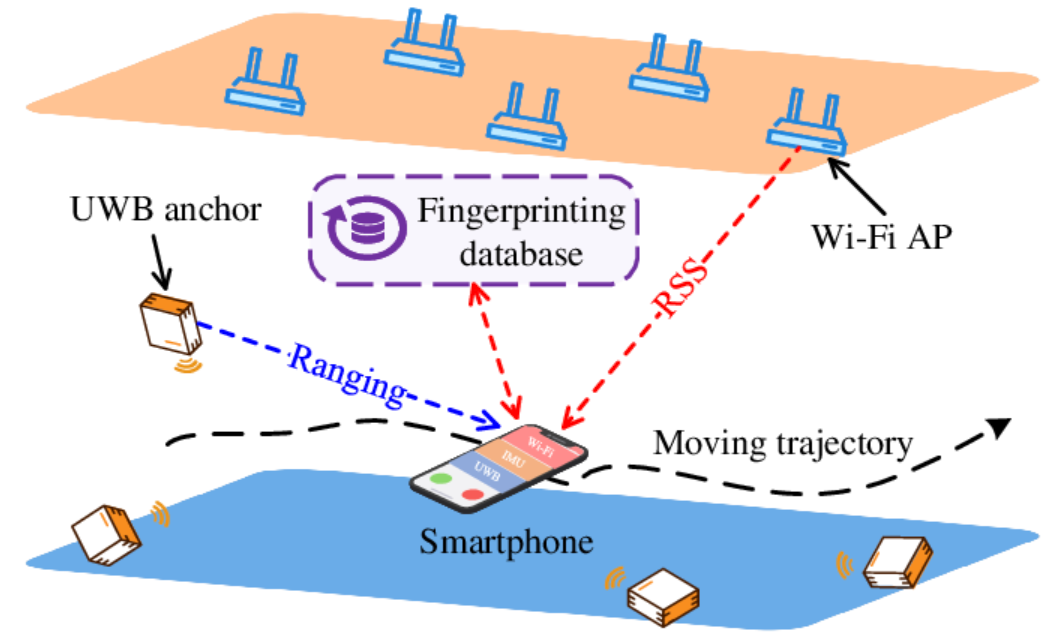
\includegraphics[width=0.8\linewidth]{images/intro.png}
  \caption{Illustration of UWB and Wi-Fi hybrid localization
    system~\cite{article}.}
  \label{fig:Illustration of UWB and Wi-Fi hybrid localization system}
\end{figure}

In addition, indoor localization technology is widely used in the medical field
for hospital material management and medical resource tracking, thereby
improving the efficiency of medical services~\cite{HOSSAIN20151}. Similarly,
emergency responders (such as firefighters) use these technologies to navigate
in complex and unfamiliar environments, significantly improving task efficiency
and safety~\cite {fischer2010location}. In addition, recent advances have
expanded the application of indoor localization systems to smart cities, helping
urban infrastructure management and public safety through real-time tracking and
monitoring of assets and personnel~\cite{zhang2020smartcity}. These technologies
have also shown significant results in the retail industry, improving the
customer experience through location-based services (such as precision marketing
and inventory management)~\cite{chen2019indoor}.

Due to the limitations of GPS in indoor environments, indoor localization
technology has become a key solution for achieving high-precision localization
due to its flexibility, adaptability, and wide range of applications. In the
following section, I introduce a new indoor localization solution and briefly
describe how it is based on Wi-Fi fingerprinting, SLAM and LiDAR fusion, and EKF
technology.

\subsection{Problem Statement}
Currently, typical indoor localization technologies each have their
characteristics and limitations. UWB technology measures the propagation time by
sending high-frequency pulse signals and has exceptionally high localization
accuracy~\cite{fontana2004recent}. However, walls and obstacles easily block UWB
radio frequency signals, and signals can rapidly attenuate, especially in indoor
environments where multipath effects are significant. In addition, UWB
technology requires high hardware costs and dense installation infrastructure,
limiting its popularity in specific applications~\cite{farahsari2022survey}.

Wi-Fi localization is a low-cost and easy-to-deploy indoor localization
technology that mainly uses Wi-Fi fingerprinting or time difference of arrival
(TDOA) methods to achieve
localization~\cite{yiu2017wireless,gustafsson2003positioning}. However, Wi-Fi
fingerprinting requires pre-measurement of signal strength at different
locations and the establishment of a fingerprint database, which is a
time-consuming and complex process. In addition, Wi-Fi signals are susceptible
to multipath effects and obstacles, resulting in reduced localization accuracy
in complex indoor environments.

IMU localization technology estimates the displacement and attitude of an object
by measuring acceleration and angular velocity. Classic IMU localization methods
include physical methods (such as double integration)~\cite{yan2018ridi}, dead
reckoning methods~\cite{jirawimut2003method}, Kalman
filtering~\cite{caron2006gps}, and sensor fusion
methods~\cite{dehzangi2017imu}. However, these methods are susceptible to error
accumulation (such as drift effects) during long-term use, resulting in a
gradual decrease in localization accuracy. Nevertheless, IMU localization
technology has high accuracy and real-time performance in a short period of
time, making it particularly suitable for fast localization tasks in dynamic
environments~\cite{marins2001improved}. In addition, IMU technology does not
rely on external infrastructure and has strong independence and reliability,
making it particularly suitable for use in environments where GPS signals cannot
be received, such as underground facilities, tunnels, or
indoors~\cite{wu2015indoor}.

Single indoor localization technologies have their advantages and disadvantages,
but by integrating multiple sensor data, especially Wi-Fi and IMU, their
limitations can be effectively compensated for, thereby achieving longer, more
continuous, and more accurate localization. Currently, most research focuses on
PDR/Wi-Fi fusion localization methods~\cite{liu2021kalman}, but IMU/Wi-Fi fusion
methods based on EKF are still rare.

\subsection{Contributions}
The objective of this study is to develop a new indoor localization system that
combines Wi-Fi, LiDAR, and EKF technologies to improve localization accuracy in
dynamic environments. Specifically, this study addresses the limitations of
existing technologies in terms of accuracy and adaptability, providing a more
powerful solution suitable for complex indoor environments.
\begin{itemize}
\item \textit{DNN-based Wi-Fi localization} : This study proposes a Wi-Fi
  localization method based on deep neural networks (DNN) that achieves higher
  accuracy in indoor localization by learning the relationship between Wi-Fi
  signal strength indicator (RSSI) and location.
    
\item \textit{Gmapping-based SLAM algorithm} : This study uses a Gmapping-based
  SLAM algorithm combined with LiDAR data to achieve efficient real-time
  localization and environment mapping, improving the system's adaptability in
  dynamic environments.
    
\item \textit{Extended Kalman filter data fusion} : This study uses EKF to fuse
  data from multiple sensors such as Wi-Fi, LiDAR, and IMU, further improving
  the accuracy and stability of the indoor localization system. In particular,
  it can effectively reduce errors and signal drift in complex dynamic
  environments.
    
\item \textit{Verification of system performance through actual experiments} :
  This study demonstrates the application effectiveness and practical
  feasibility of the proposed system in complex indoor scenarios through
  experiments conducted in actual indoor environments.
\end{itemize}

\subsection{Thesis Outline}
This thesis is divided into six parts. The first part is the introduction, which
provides the overall background and motivation for the project. The second part
is a literature review, which comprehensively reviews the progress of indoor
localization technology, data set construction, sensor fusion methods, and the
application of EKF in indoor localization. The third part introduces in detail
the specific methods used in this study, including Wi-Fi localization, LiDAR
data processing, and EKF data fusion technologies. The fourth part presents the
experimental results and evaluates the localization accuracy and stability of
the system in different environments. The fifth part discusses the results of
the entire project, analyzes the advantages and limitations of the method, and
proposes directions for improvement. Finally, the sixth part summarizes the main
contributions of this research and gives prospects for future research.


\newpage
\section{Literature Review}
In recent years, indoor localization technology has gradually become a hot topic
of research in academia and industry due to its key role in applications such as
smart city construction, indoor navigation, and the Internet of Things
(IoT)\nomenclature{IOT}{Internet of Things}. The performance of localization
systems in terms of accuracy, robustness, and system scalability directly
affects their usability and deployment efficiency in real-world scenarios. With
the continuous advancement of sensor technology, wireless communication, and
intelligent algorithms, research in this field is showing a multidimensional
trend toward integration, intelligence, and high precision.

\subsection{Advances in indoor localization technology without calibration}
Traditional indoor localization methods, such as Wi-Fi or Bluetooth-based
fingerprinting systems, typically rely on prior site surveys to construct radio
frequency (RF) maps. This process is both time-consuming and labor-intensive,
and highly sensitive to environmental changes, limiting its scalability and
adaptability~\cite{liu2020survey}. Additionally, as environmental factors change
(e.g., furniture rearrangement), the data from site surveys often becomes
outdated, significantly impacting system performance~\cite{jiang2019indoor}.

To overcome these limitations, researchers have proposed calibration-free indoor
localization systems. These systems avoid cumbersome site surveys by
constructing RF maps using existing infrastructure or with the implicit
participation of users, thereby greatly reducing deployment time and costs while
improving system flexibility in dynamic
environments~\cite{HOSSAIN20151,li2018calibrationfree}.

Although systems that do not require calibration offer significant advantages,
they still face challenges in adapting to environmental changes and handling
device heterogeneity. As emphasized by Hossain and Soh, changes in the physical
environment and differences in device hardware can affect the accuracy of
localization systems, posing a significant challenge for current
technologies~\cite{HOSSAIN20151}. To address these issues, researchers have
proposed several improvements, including dynamically updating RF maps and using
advanced optimization algorithms to enhance system robustness and
reliability~\cite{zhang2020robust}.

Advances in these technologies have enabled calibration-free indoor localization
technologies to be widely used in complex commercial and public
environments. For example, in large shopping malls, hospitals, museums, and
multi-story office buildings, the deployment and long-term maintenance of
traditional localization methods are difficult due to complex building
structures, high personnel mobility, and wireless signal interference. However,
calibration-free systems can quickly adapt to these changing environments and
provide accurate localization services by utilizing existing wireless
infrastructure (such as Wi-Fi or Bluetooth) and data from mobile devices (such
as smartphones)~\cite{laoudias2018survey,xu2019wireless}.

\subsection{Construction and application of long-time data sets}
One of the core challenges facing indoor localization research is the volatility
of signal strength over time. Factors such as access point configuration
changes, dynamic environmental changes (e.g., crowd density, furniture
movement), and device heterogeneity can significantly affect the stability and
accuracy of traditional fingerprint-based localization
systems~\cite{liu2020survey}. Therefore, how to maintain localization accuracy
in dynamic environments over long periods of time has become an urgent issue.

In response to this challenge, recent research has emphasized the importance of
building long-term datasets to capture the evolution of signals over
time. Mendoza-Silva et al.~\cite{data3010003} provided a Wi-Fi fingerprint
dataset collected over 15 months, systematically revealing the long-term impact
of factors such as network device replacement and environmental structure
changes on the performance of localization systems. The study shows that
incorporating long-term signal data into a fingerprint database and updating it
dynamically can significantly improve the system's ability to adapt to
environmental changes, thereby reducing localization errors caused by signal
attenuation or configuration drift.

To achieve real-time adaptation, many scholars have proposed mechanisms for
dynamically updating fingerprint databases. For example, Zhang et
al.~\cite{zhang2019dynamic} and Bahl et al.~\cite{10.1145/2568225.2568272}
proposed using time modeling and online learning algorithms to dynamically
maintain RF maps, enabling the system to respond in real time to changes in the
signal environment and avoid the accuracy degradation issues commonly found in
static fingerprint systems.  The combination of long-term data sets and adaptive
updating mechanisms has greatly improved the robustness and reliability of
localization systems. In particular, in highly dynamic real-world scenarios such
as multi-story buildings, shopping malls, or large transportation hubs, this
strategy can ensure that the system continues to provide high-precision
localization services~\cite{sen2013you, shang2015enhancing}, effectively
responding to the challenges brought about by environmental uncertainty and
changes.

\subsection{Combination of deep learning and multi-sensor fusion}
In recent years, deep learning technology has made breakthroughs in fields such
as computer vision and natural language processing. Inspired by this,
researchers have begun to introduce it into indoor localization systems,
especially in scene recognition and precise localization tasks in complex
environments. Unlike traditional methods that rely on static fingerprint
matching, deep learning can automatically extract multi-level features from
multi-sensor data through neural networks, model more complex spatial patterns,
and thus improve the system's adaptability and robustness~\cite{s151229867,
  nowicki2017ml}.

Liu et al. proposed an indoor localization method that integrates deep
convolutional neural networks (CNNs)~\nomenclature{CNNs}{convolutional neural
  networks} and multi-sensor data~\cite{s151229867}. This method is based on
Wi-Fi, magnetic field, and inertial sensor data for indoor scene recognition,
and estimates the user's location through a particle filtering
algorithm. Experimental results show that this method can control the
localization error within 1.32 meters at a 95\% confidence level, which is
significantly better than traditional fingerprint matching technology in dynamic
environments. At the same time, this method effectively alleviates the signal
ambiguity caused by environmental changes and improves the generalization
ability of the system.

Traditional fingerprint localization methods rely on a pre-collected signal
strength fingerprint database and estimate the location by matching it with
real-time observation signals~\cite{ijgi6050135}. Although these methods perform
well in relatively stable environments, they face several limitations: on the
one hand, static fingerprint databases cannot dynamically adapt to environmental
changes, such as wireless device replacement or changes in personnel density; on
the other hand, these methods are highly sensitive to signal interference and
multipath effects, often resulting in significant errors in multi-story
buildings or densely populated areas~\cite{zou2022magloc}.

In contrast, deep learning methods can learn robust spatial features from
heterogeneous sensor data with the help of neural networks and adapt to
environmental changes through incremental learning or online updates, thereby
effectively maintaining localization accuracy. For example, Nowicki and
Wietrzykowski proposed a CNN-based Wi-Fi fingerprint localization method that
outperformed traditional methods in multiple scenarios~\cite{nowicki2017ml}. In
addition, Zhou et al. introduced long short-term memory (LSTM) networks to
perform time modelling of multi-sensor signals, achieving real-time adaptive
localization in complex dynamic environments~\cite{zhou2022deep}.

\subsection{Extended Kalman filter in indoor localization}
Extended Kalman filters are widely used in indoor localization systems as
real-time recursive estimators that can fuse noisy, asynchronous, and multimodal
sensor data within a probabilistic framework. Unlike the standard Kalman filter,
which is only applicable to linear systems, the EKF linearizes nonlinear motion
and observation models through a first-order Taylor expansion, enabling it to
handle nonlinear motion and observation models. This makes it particularly
suitable for indoor environments, where user trajectories, sensor measurements,
and signal propagation are inherently nonlinear~\cite{barrau2015non}.

In Wi-Fi-based localization scenarios, EKF is often used to refine location
estimates based on noisy RSSI or channel state information observations. When
fused with other modalities such as IMU and LiDAR, EKF can integrate absolute
and relative localization information, thereby improving localization accuracy
and temporal continuity~\cite{laoudias2018survey}. For instance, the WIO-EKF
method proposed by Zhou and Wang (2023) combines Wi-Fi fingerprint and IMU
data~\cite{zhou2024wio}. It fuses them using EKF to provide more accurate and
continuous pedestrian localization. The innovation of this method lies in that
it not only solves the initial heading error problem of IMU, but also enhances
the localization results using Wi-Fi fingerprint data. Specifically, the WIO-EKF
method first enhances Wi-Fi fingerprint data using the CDAELoc model (a
regression network based on convolutional denoising
autoencoders)\nomenclature{CDAE}{Convolutional Denoising Autoencoders} to
improve the robustness of Wi-Fi localization in noisy environments. Then, the
DbDIO model (a dual-branch deep inertial odometer network)
\nomenclature{DbDIO}{Dual-branch Deep Inertial Odometer}is used to process IMU
data and accurately extract features of different scales. The prediction results
of these models are input as system observations into the EKF, thereby reducing
the initial heading error of the IMU system.

\subsection{Multisensor fusion technology in indoor localization systems}
With the continuous evolution of indoor localization technology, traditional
localization methods that rely on a single signal source face significant
challenges in terms of accuracy and robustness in complex environments. In order
to improve the stability and adaptability of the system in dynamic and
interference-prone environments, multi-sensor fusion technology has gradually
become an important direction for indoor localization system research and
application. This technology integrates data sources from different types of
sensors to achieve more accurate, continuous, and robust estimation of the
target location.

Multi-sensor fusion can be categorized into three typical architectures:
data-level fusion, feature-level fusion, and decision-level fusion. Data-level
fusion directly integrates raw sensor data, retaining the most complete
information, but requires high time synchronization and noise
robustness. Feature-level fusion combines features extracted independently by
each sensor, balancing complexity and efficiency. Decision-level fusion performs
final estimation through weighted voting or filtering strategies after each
subsystem completes localization inference, and is suitable for heterogeneous or
distributed systems~\cite{zafari2019survey}.

Currently, multi-sensor fusion is mainly reflected in several key application
paths: First, Wi-Fi and IMU fusion compensates for the drift of Wi-Fi
localization in short-term dynamic changes through inertial measurement units
(such as accelerometers and gyroscopes) and is widely used in areas without GPS
signal coverage~\cite{liu2019fusion}. Second, UWB and vision (camera or LiDAR)
fusion is suitable for industrial scenarios or robot path planning and and can
achieve centimeter-level localization accuracy~\cite{gu2020fusion}; third, deep
learning-assisted fusion frameworks learn the nonlinear relationships between
multimodal features in end-to-end models through neural networks to achieve
robust perception and localization in complex environments~\cite{zhou2022deep}.

Although fusion technology has significantly improved the performance of
localization systems, many challenges remain~\cite{zafari2019survey}. First, the
issues of time synchronization, coordinate alignment, and scale consistency
between different sensors have not been completely resolved. Second, given the
limited computing power of mobile devices, the computational complexity and
energy efficiency optimisation of fusion algorithms still need to be
balanced. Finally, multi-sensor systems face practical deployment challenges
such as data heterogeneity and outlier handling, which affect their feasibility
in large-scale, low-cost application scenarios.


\newpage
\section{Methodology}
\subsection{Data processing and integration process}
In order to achieve a high-precision and robust indoor localization system, this
thesis designs and implements a localization method framework that integrates
information from multiple sensors. The overall process covers the entire process
from raw data collection and information fusion processing to localization
result optimization. The system uses multiple sensors such as Wi-Fi, LiDAR, and
IMU for collaborative localization, and realizes multi-source data fusion and
optimization estimation through the EKF algorithm.

The entire data acquisition and fusion process is divided into several steps:
First, data from different sensors (such as Wi-Fi signals, SLAM maps, and IMU
data) are collected, preprocessed, and stored in a database. Then, these data
are fused and optimized through the EKF algorithm to ultimately achieve accurate
localization estimation. \autoref{fig:Flowchart of multi-sensor localization
  system} shows the detailed steps of data acquisition, sensor data fusion, and
localization result optimization\nomenclature{ROS}{Robot Operating System}.
\begin{figure}[H]
  \centering
  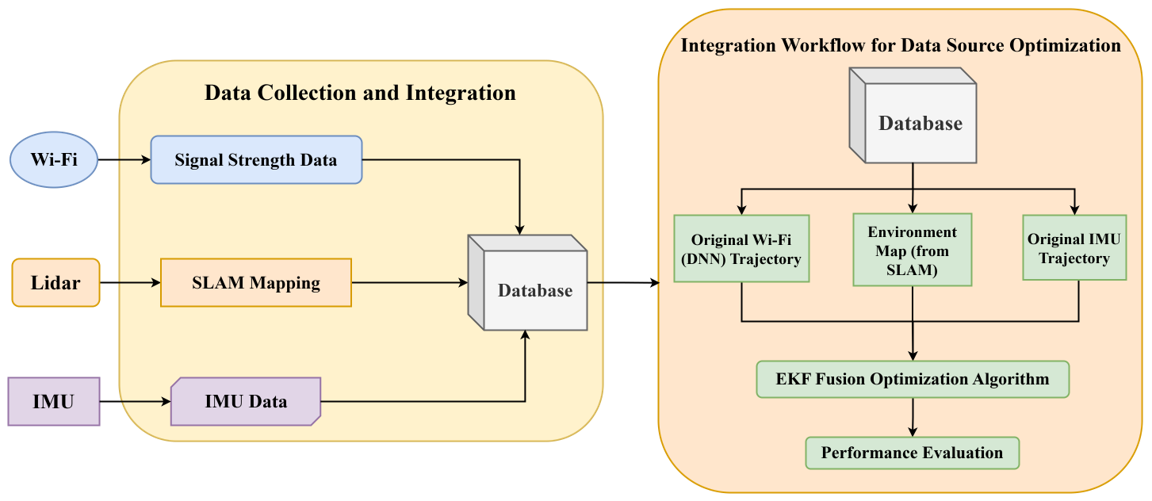
\includegraphics[width=\linewidth]{images/Overview_plus.png}
  \caption{Overall architecture and information processing flow of a
    multi-sensor cooperative localization system.}
  \label{fig:Flowchart of multi-sensor localization system}
\end{figure}

In the next section, I introduce the deployment and integration of this
localization system on an autonomous mobile platform, including the hardware and
software architecture design, module docking process, and system operation
mechanism, thereby verifying the applicability and feasibility of this method in
a real environment.

\subsection{Hardware design}
The localization system in this study is deployed on a mobile autonomous
platform, namely an autonomous guided vehicle (AGV)\nomenclature{AGV}{Autonomous
  Guided Vehicle}, which serves as a carrier for multi-sensor data acquisition
and real-time localization. As shown in~\autoref{fig:Hardware platform
  components of AGV}, the AGV platform consists of three main components: a
mobile chassis system, a sensor module, and an edge computing unit. Among them,
the mobile chassis is equipped with differential drive motors and wheel
encoders, which provide good steering flexibility and motion stability, enabling
smooth movement and path tracking in indoor environments. The sensor module
integrates a two-dimensional \hl{laser radar}, IMU, Wi-Fi receiver, and depth camera
to perceive the environmental structure, capture its dynamic state, and obtain
wireless signal information. The computing core of the system consists of edge
computing units (such as NVIDIA Jetson and Raspberry Pi), which are responsible
for local data collection and processing.
%%%
\comment{Joseph}{Is the ``laser radar'' different from LiDAR?}%
%%%

The entire platform is compact in design and easy to deploy flexibly in
multi-story and multi-scenario environments, providing a good hardware
foundation for subsequent large-scale localization experiments and system
expansion. After data collection is complete, one of the core issues of this
research is how to efficiently integrate data from different sensors to ensure
localization accuracy and robustness.
\begin{figure}[H]
  \centering
  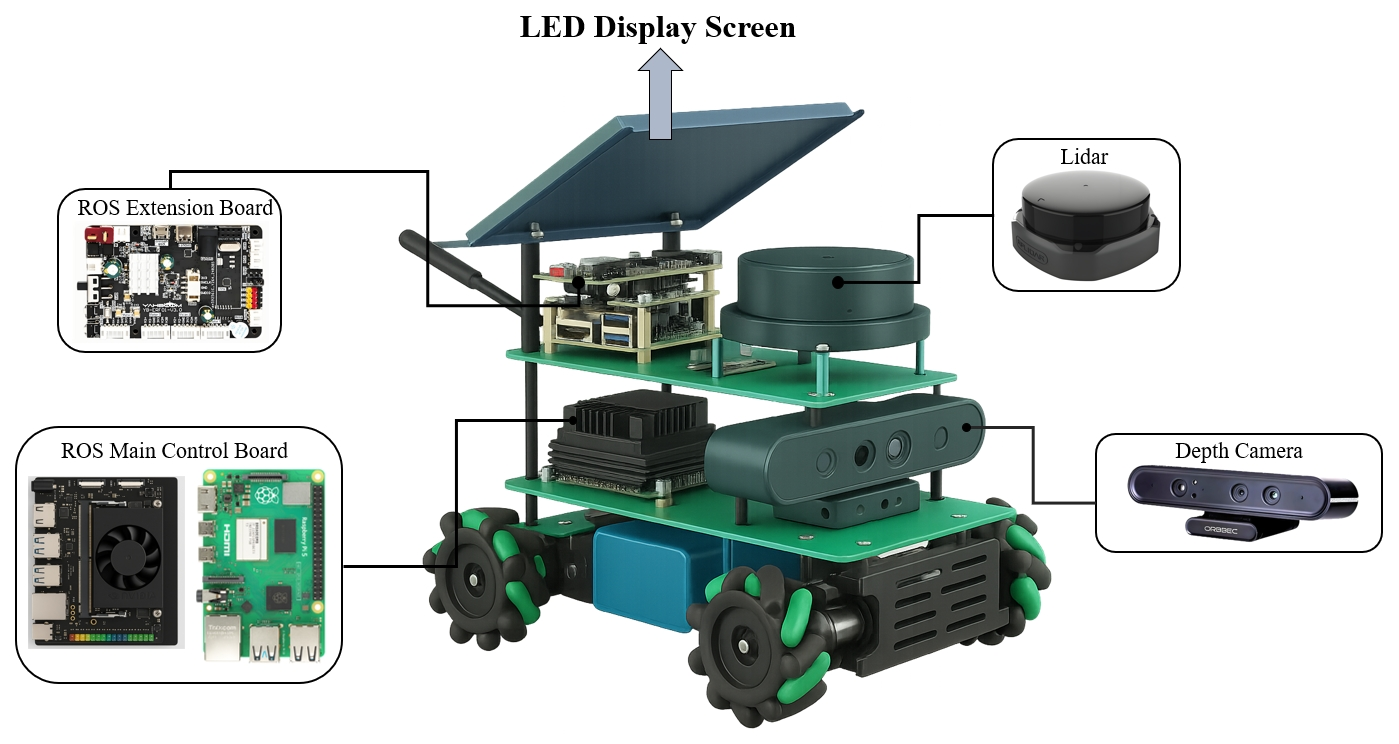
\includegraphics[width=0.95\linewidth]{images/Hardware.png}
  \caption{Hardware platform components of AGV.}
  \label{fig:Hardware platform components of AGV}
\end{figure}

\subsection{Wi-Fi Fingerprint-based localization using Deep Neural Networks }
On the basis of multi-source data collection and system integration, this study
further constructed a Deep Neural Networks (DNNs) model based on Wi-Fi Received
Signal Strength Indicator (RSSI)
% \nomenclature{RSSI}{Received Signal Strength Indicator}
fingerprints to achieve regression prediction of the platform's
two-dimensional location. The model aims to characterize the nonlinear mapping
relationship between RSSI signal strength and physical space coordinates, and to
model high-dimensional RSSI feature vectors through a supervised learning
framework, thereby achieving high-precision indoor localization.

As shown in~\autoref{fig:Workflow of the Wi-Fi Fingerprint-Based DNN
  Localization Framework}, the overall process of the Wi-Fi localization
subsystem is divided into four stages: data preparation, feature modelling,
model training and prediction, and performance evaluation, which constitute a
complete fingerprint-based localization method.
\begin{figure}[H]
  \centering
  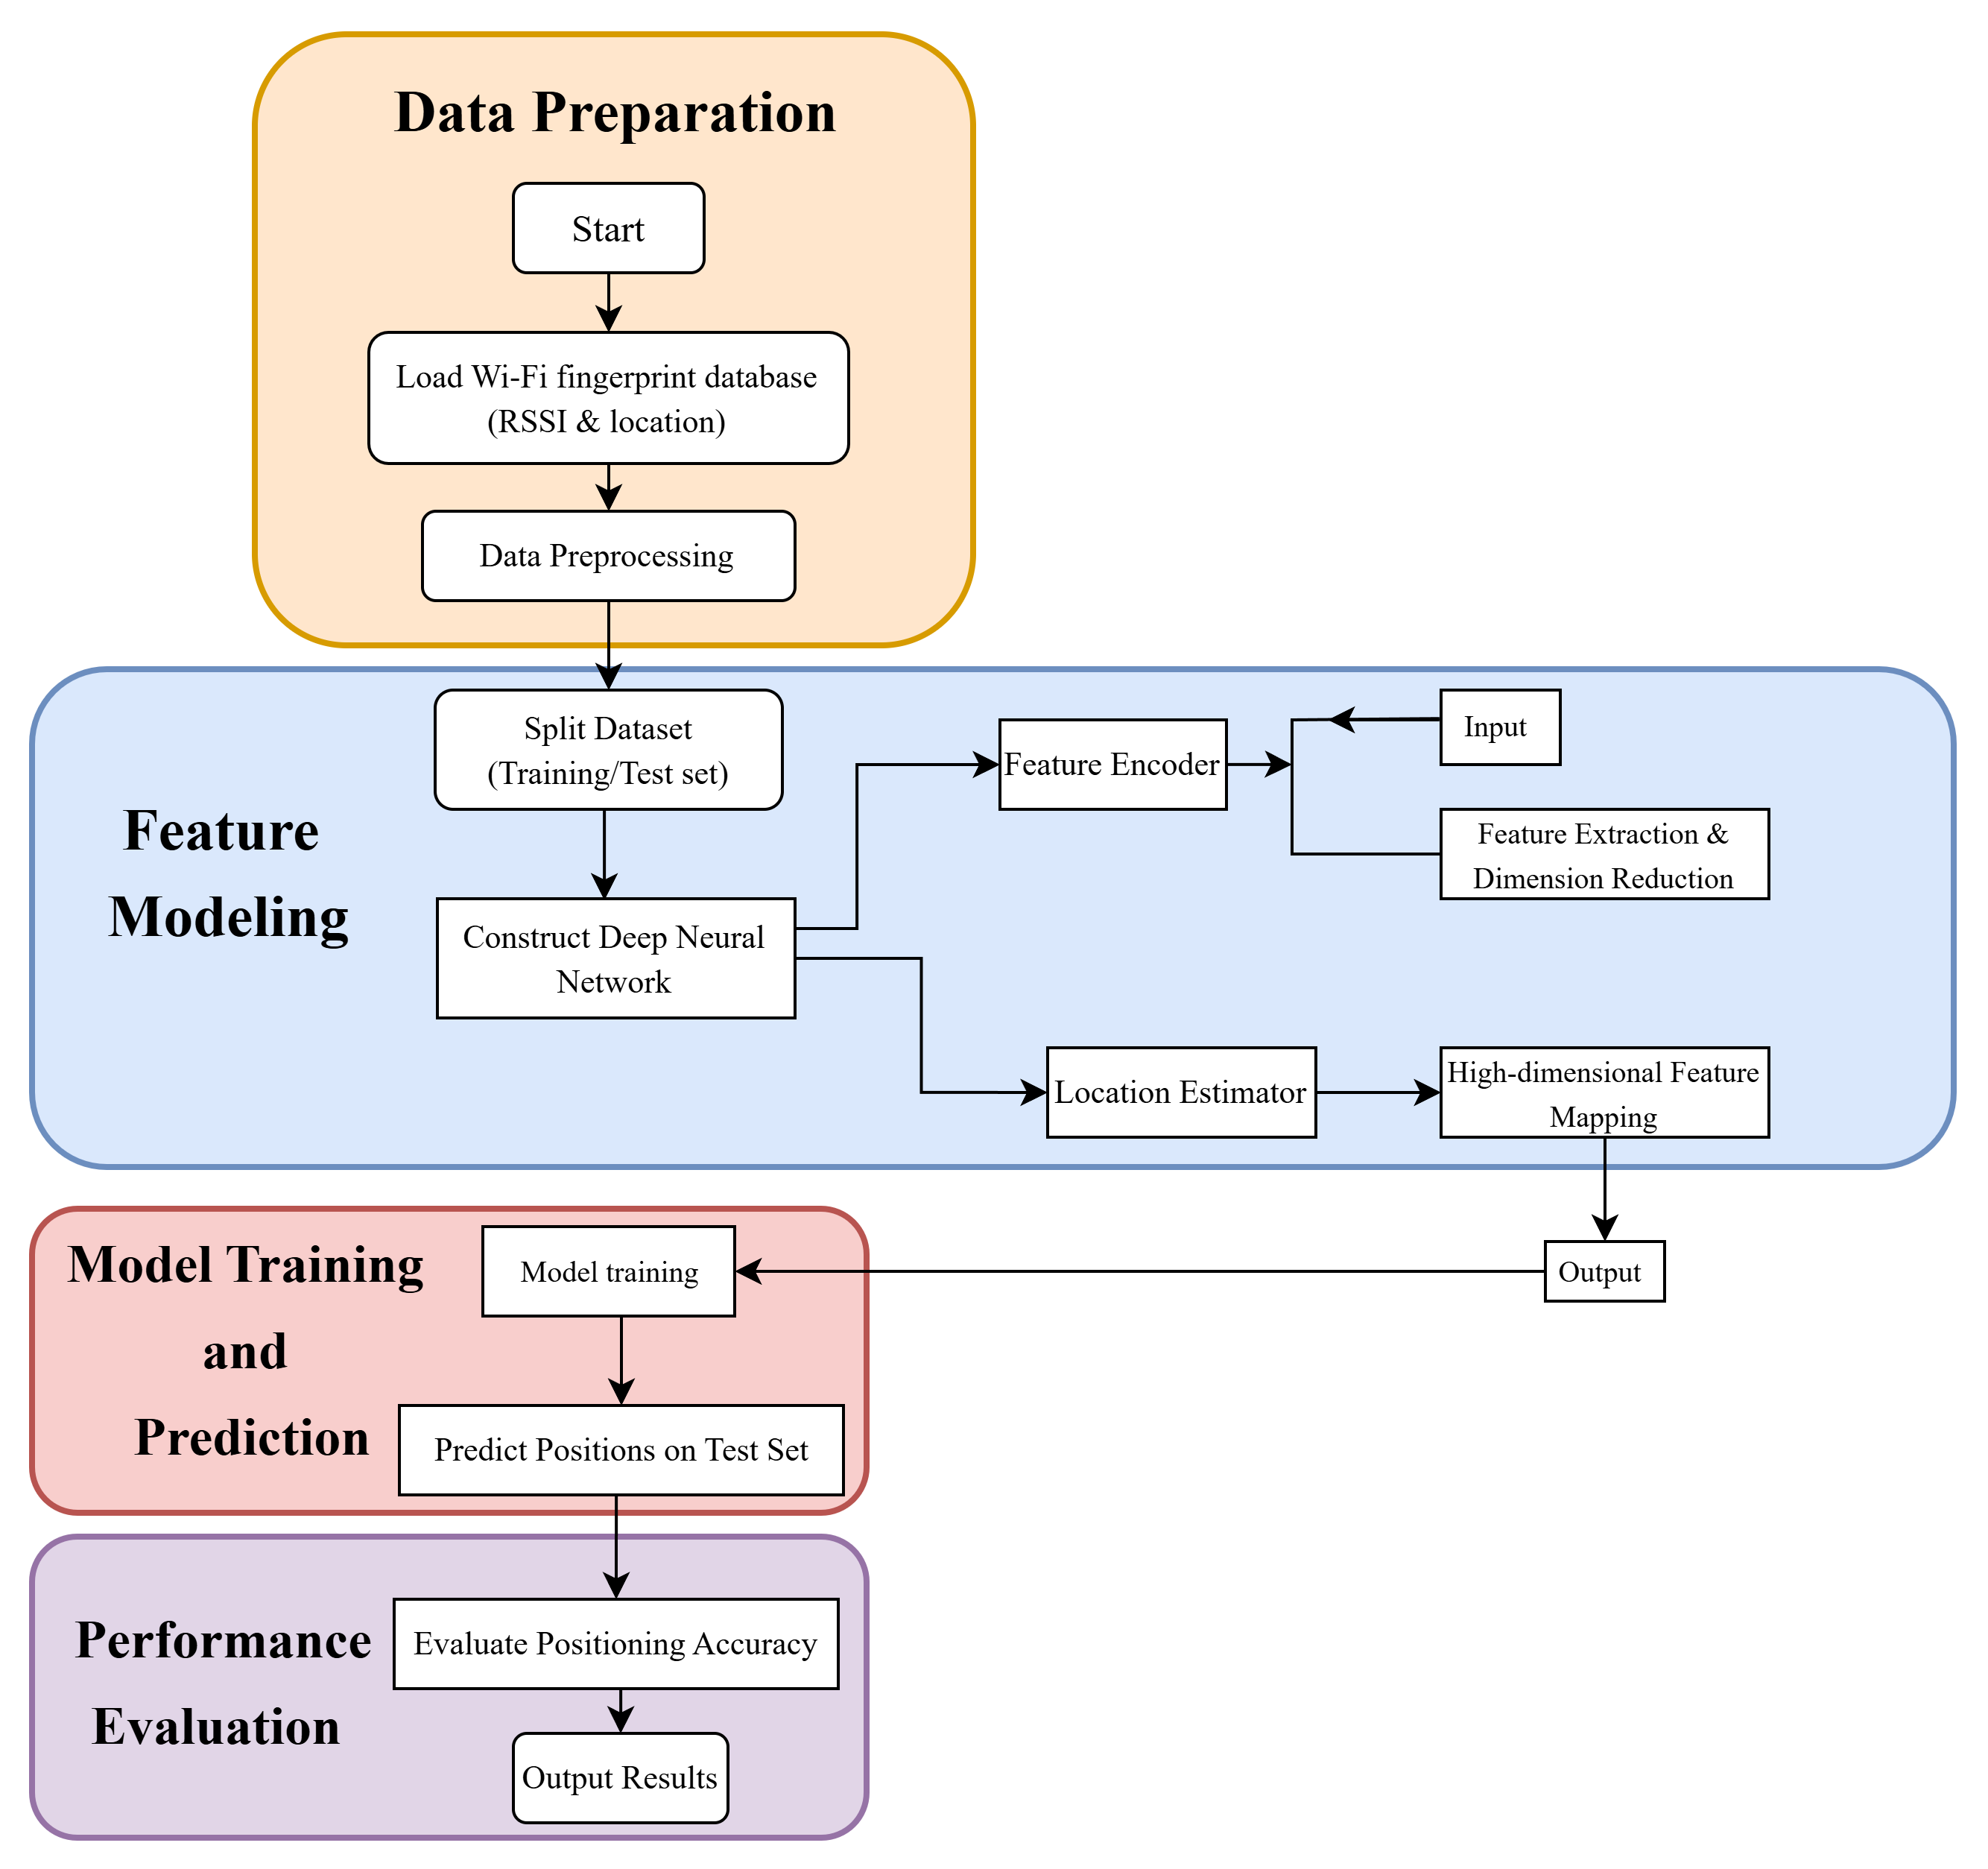
\includegraphics[width=0.8\linewidth]{images/2.png}
  \caption{Workflow of the Wi-Fi Fingerprint-Based DNN Localization Framework.}
  \label{fig:Workflow of the Wi-Fi Fingerprint-Based DNN Localization Framework}
\end{figure}

First, the system loads a pre-built fingerprint database, which contains RSSI
vectors collected at different reference points and their corresponding physical
coordinate labels. To improve modelling quality and convergence stability, the
raw data is preprocessed, including missing value filling, feature
normalization, and outlier removal. After preprocessing, the data is divided
into training and testing sets for subsequent model learning and generalization
capability verification.

In the modelling phase, this study designed a multi-layer feedforward neural
network structure to extract spatial features from high-dimensional RSSI
fingerprints and perform location regression prediction. The model consists of
multiple linear layers, Rectified Linear Unit (ReLU), and dropout layers,
constructed using a layered stacking method of “Linear-ReLU-Dropout.” The
input dimension of the network is 219, corresponding to the number of active
access points (AP) \nomenclature{AP}{Access Point}, and the output is a
two-dimensional coordinate value (x, y). The complete network layer structure is
shown in~\autoref{tab:wifi_dnn_structure}. This structure can effectively
extract potential spatial distribution patterns in the signal space and achieve
mapping from the signal domain to the physical domain.
\nomenclature{ReLU}{Rectified Linear Unit}
\begin{table}[H]
  \centering
  \caption{Architecture of the Wi-Fi fingerprint-based DNN model}
  \label{tab:wifi_dnn_structure}
  \begin{tabular}{ccccc}
    \toprule
    \textbf{Layer} & \textbf{Type} & \textbf{Input Dim} & \textbf{Output Dim} & \textbf{Activation / Dropout} \\
    \midrule
    1 & Linear & 219  & 109 & ReLU + Dropout(0.2) \\
    2 & Linear & 109  & 73  & ReLU + Dropout(0.2) \\
    3 & Linear & 73   & 54  & ReLU + Dropout(0.2) \\
    4 & Linear & 54   & 109 & ReLU + Dropout(0.2) \\
    5 & Linear & 109  & 109 & ReLU + Dropout(0.2) \\
    6 & Linear & 109  & 109 & ReLU + Dropout(0.2) \\
    7 & Linear & 109  & 2   & None \\
    \bottomrule
  \end{tabular}
\end{table}

During the model training process, the mean squared error (MSE)
\nomenclature{MSE}{Mean Squared Error} is used as the loss function, and the
Adam optimizer is used to update the model parameters. In the testing phase, the
model receives RSSI vector input and outputs the location prediction
results. Then, the average localization error is calculated by comparing the
Euclidean distance between the predicted location and the actual coordinates to
evaluate the model's performance.

Overall, as an essential part of the localization system, the Wi-Fi fingerprint
localization framework not only provides prior trajectory information for the
subsequent fusion stage but also demonstrates good robustness and generalization
ability, making it suitable for a variety of complex and dynamically changing
indoor environments.

\subsection{LiDAR-based SLAM and IMU Integration}
Although Wi-Fi fingerprint-based deep neural network models can achieve
relatively accurate location estimates in static environments, they still face
many challenges in complex indoor environments, including severe RSSI
fluctuations, multipath propagation, signal obstruction, and high fingerprint
database update costs. These factors can easily lead to a decline in model
generalization performance, especially in areas with sparse or dynamically
changing signals, where it is difficult for the system to maintain continuous
and stable localization output.

To enhance the system's environmental perception and spatial understanding
capabilities, this study introduces the SLAM method. SLAM can construct an
environmental map and perform self-localization in real time by processing
sensor observation data in the absence of prior maps, and is widely used in
mobile robots and indoor navigation systems~\cite{durrant2006slam}. Its core
idea is to dynamically update the environment representation while estimating
the platform trajectory, thereby achieving joint inference of space and motion.

In this system, we specifically adopted the particle filter-based Gmapping
algorithm. Gmapping uses Rao-Blackwellized particle filtering technology to fuse
two-dimensional laser radar scan data with wheel odometer information, and
utilizes a probabilistic grid mapping method to generate a closed-loop
consistent, high-resolution two-dimensional environmental map, and outputs
high-precision pose trajectory estimates~\cite{grisetti2007improved}. Compared
with other methods, Gmapping has the advantages of mature implementation, low
computational resource consumption, and strong closed-loop detection
capabilities, making it particularly suitable for real-time mapping tasks in
small and medium-sized indoor scenes.

\autoref{fig:SLAM Mapping Results on the 6th, 7th and 8th Floors of the IR
  Building} shows the environment map results obtained by the system when
performing SLAM mapping on the 6th, 7th, and 8th floors of the IR building at
Xi'an Jiaotong-Liverpool University (XJTLU). The results clearly reproduce the
floor structure and reflect the coverage area of the laser scan.
\begin{figure}[H]
  \centering
  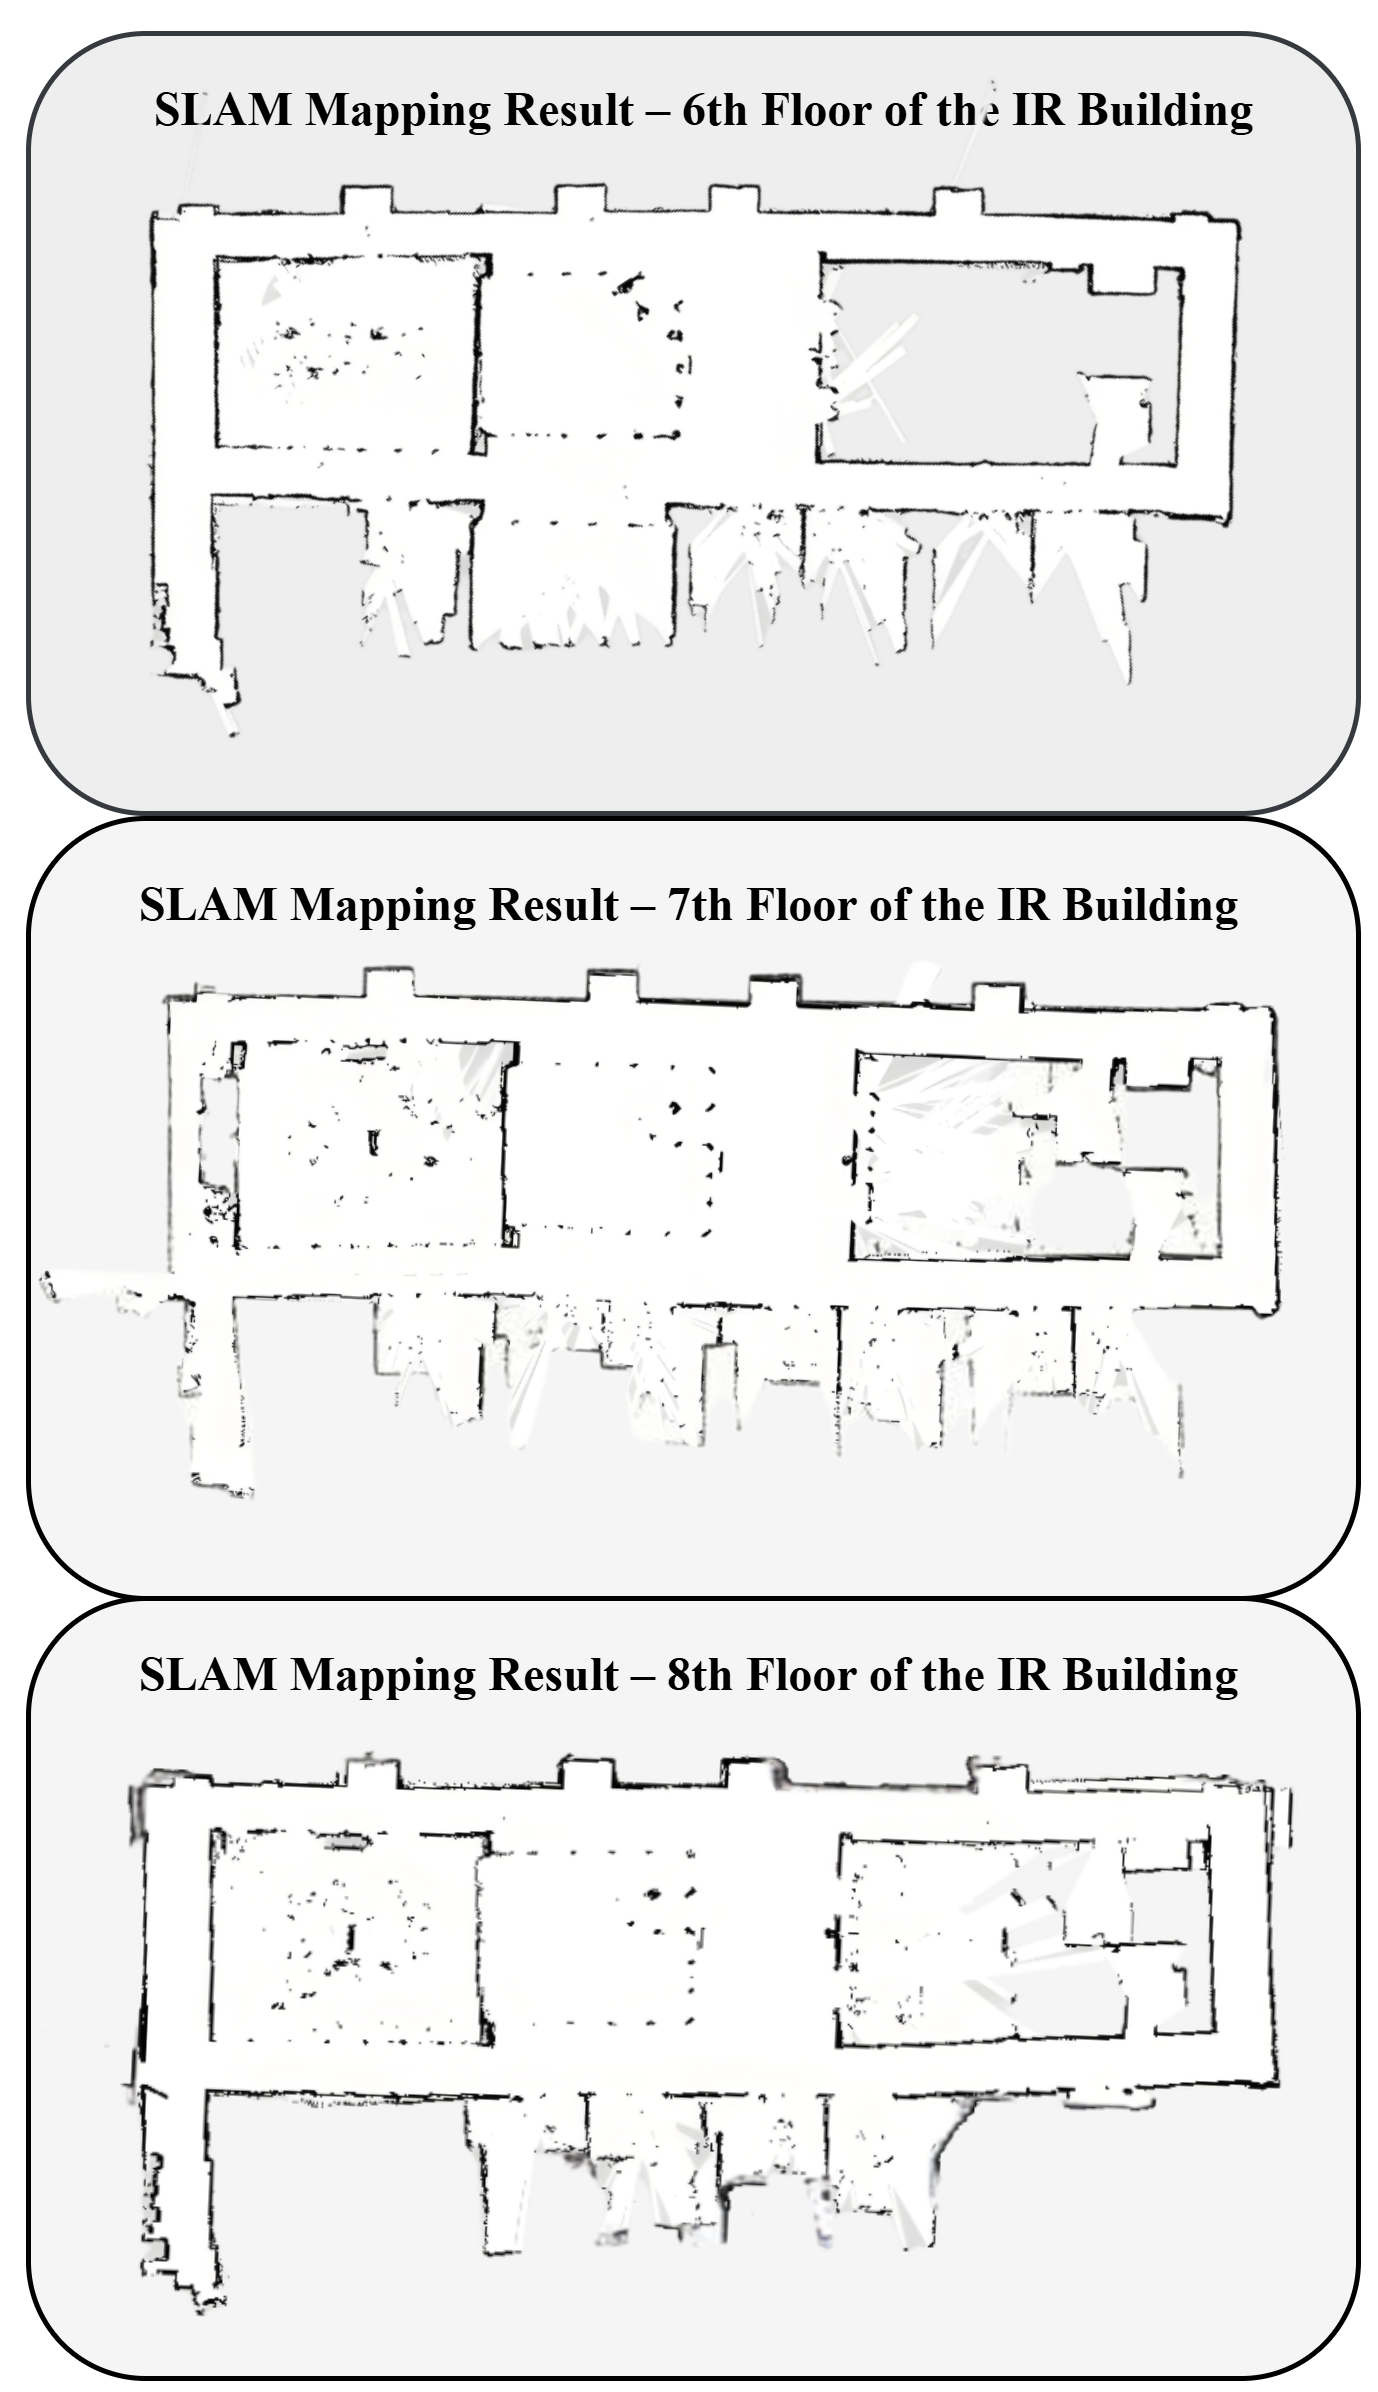
\includegraphics[width=0.48\linewidth]{images/slam.png}
  \caption{SLAM mapping results for three floors of the IR building.}
  \label{fig:SLAM Mapping Results on the 6th, 7th and 8th Floors of the IR
    Building}
\end{figure}

For further improvement of the system's dynamic response capabilities under
conditions of rapid movement, turning, and partial obstruction, an IMU is
integrated into the localization system as an auxiliary sensor. IMU usually
includes a three-axis accelerometer and a three-axis gyroscope, which are used
to measure linear acceleration and angular velocity. Through integration, the
attitude changes and displacement information of the platform in a short period
of time can be estimated.
\begin{equation}
  \boldsymbol{a} =
  \begin{bmatrix}
    a_x \\ a_y \\ a_z
  \end{bmatrix}, \quad
  \boldsymbol{\omega} =
  \begin{bmatrix}
    \omega_x \\ \omega_y \\ \omega_z
  \end{bmatrix}
\end{equation}
where $a_x, a_y, a_z$ denote the accelerations along the x-, y-, and z-axes,
respectively. $\omega_x, \omega_y, \omega_z$ denote the angular velocities about
the x-, y-, and z-axes, respectively.

In the modelling process, IMU observation data is represented as:
\begin{equation}
  \boldsymbol{a}_{\text{meas}} = \boldsymbol{a}_{\text{true}} + \boldsymbol{b}_a + \boldsymbol{n}_a,
  \quad
  \boldsymbol{\omega}_{\text{meas}} = \boldsymbol{\omega}_{\text{true}} + \boldsymbol{b}_\omega + \boldsymbol{n}_\omega
\end{equation}
where, $\boldsymbol{\alpha}_{\text{meas}}$ denotes the observed acceleration,
$\boldsymbol{\alpha}_{\text{true}}$ denotes the true acceleration, ${b}_\alpha$
denotes the zero bias, and ${n}_\alpha$ denotes the noise term. Similarly,
$\boldsymbol{\omega}_{\text{meas}}$ represents the measured angular velocity,
$\boldsymbol{\omega}_{\text{true}}$ is the true angular velocity, ${b}_\omega$
is the corresponding bias, and ${n}_\omega$ accounts for measurement
noise. These sources of error are modelled and corrected during the fusion stage
using the EKF to improve localization stability and accuracy. The high sampling
frequency of the IMU enables it to effectively compensate for the shortcomings
of LiDAR in short-term motion estimation, improving the localization continuity
and robustness of the system in highly dynamic environments.

Overall, the integration of SLAM and IMU not only provides a solid foundation
for the system to construct an environmental map and provide continuous
trajectory estimation, but also provides structured and dynamic compensation
multi-source perception support for subsequent fusion optimization with Wi-Fi
trajectories.

\subsection{Multi-Sensor fusion via Extended Kalman Filter}
This study further constructs a fusion framework based on the EKF to achieve
effective coordination and information complementarity among subsystems. The
fusion model is centered on state space modelling, integrating pose information
from Wi-Fi fingerprint localization, SLAM module outputs, and short-term
high-frequency motion observations provided by IMU sensors to achieve dynamic
estimation and real-time correction of the platform state.

In the specific implementation, the EKF models the nonlinear motion system as a
recursive prediction-update structure, alternately completing the two stages of
state estimation and observation correction. The prediction stage infers the
future state of the system based on the state at the previous moment and the
control input, while the update stage corrects the state based on sensor
observations, thereby continuously improving the estimation accuracy. This
filtering structure has been widely applied in multi-sensor fusion localization
and demonstrates good robustness in addressing issues such as IMU drift and RSSI
instability~\cite{zhuang2023multi}.

The recursive process of the overall state estimation is shown
in~\autoref{fig:EKF State Prediction and Observation Update Flowchart} below.
\begin{figure}[H]
  \centering
  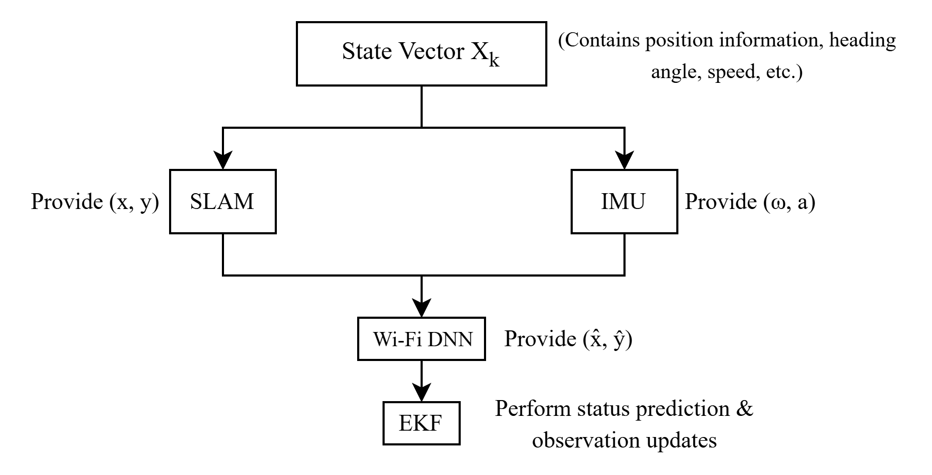
\includegraphics[width=0.85\linewidth]{images/图片1.png}
  \caption{EKF State Prediction and Observation Update Flowchart.}
  \label{fig:EKF State Prediction and Observation Update Flowchart}
\end{figure}

All formulas in this section are based on the EKF model structure and state
estimation framework proposed in the literature
\cite{bailey2006consistency,lerro1993tracking,li2013high} and are used to model
the multi-sensor data fusion process.

To establish a unified estimation system, it is first necessary to define the
system state vector and its evolution relationship. In this study, the system
state estimated by the EKF is defined as
\begin{equation}
  \mathbf{X}_k =
  \begin{bmatrix}
    x_k \\
    y_k \\
    \theta_k \\
    v_k \\
    \omega_k
  \end{bmatrix}
  \label{eq:Xk_definition}
\end{equation}
where the platform's position $(x_k, y_k)$ in the two-dimensional plane, heading
angle $\theta_k$, linear velocity $v_k$, and angular velocity $\omega_k$,
constituting a complete description of the motion characteristics.

Different from traditional methods, which typically estimate only
two-dimensional locations as state variables~\cite{li2006indoor}, this study
further introduces dynamic motion parameters (velocity and angular velocity),
enhancing the system's ability to model continuous trajectories, especially in
highly dynamic or complex path environments, with stronger
robustness~\cite{sun2019fusion}.

Specifically, the two-dimensional location estimation $(x_k, y_k)$ of the
platform is mainly obtained by the Wi-Fi fingerprint localization module through
RSSI vector modelling. Although its update frequency is low, it has good global
stability and long-term consistency. The SLAM module outputs the estimated
results of the mid-frequency trajectory containing the position and orientation
angle $\theta_k$ through the joint mapping of the laser radar and odometer,
providing structured spatial constraints for the system. The linear velocity
$v_k$ and angular velocity $\omega_k$ of the platform are mainly derived from
the high-frequency dynamic measurements of the accelerometer and gyroscope in
the IMU module, which can be used for short-term motion inference and
compensation in the state prediction phase. The relationship between each
subsystem and the state vector is shown in~\autoref{fig:Structural diagram of
  EKF input and status vector composition} below.
\begin{figure}[H]
  \centering
  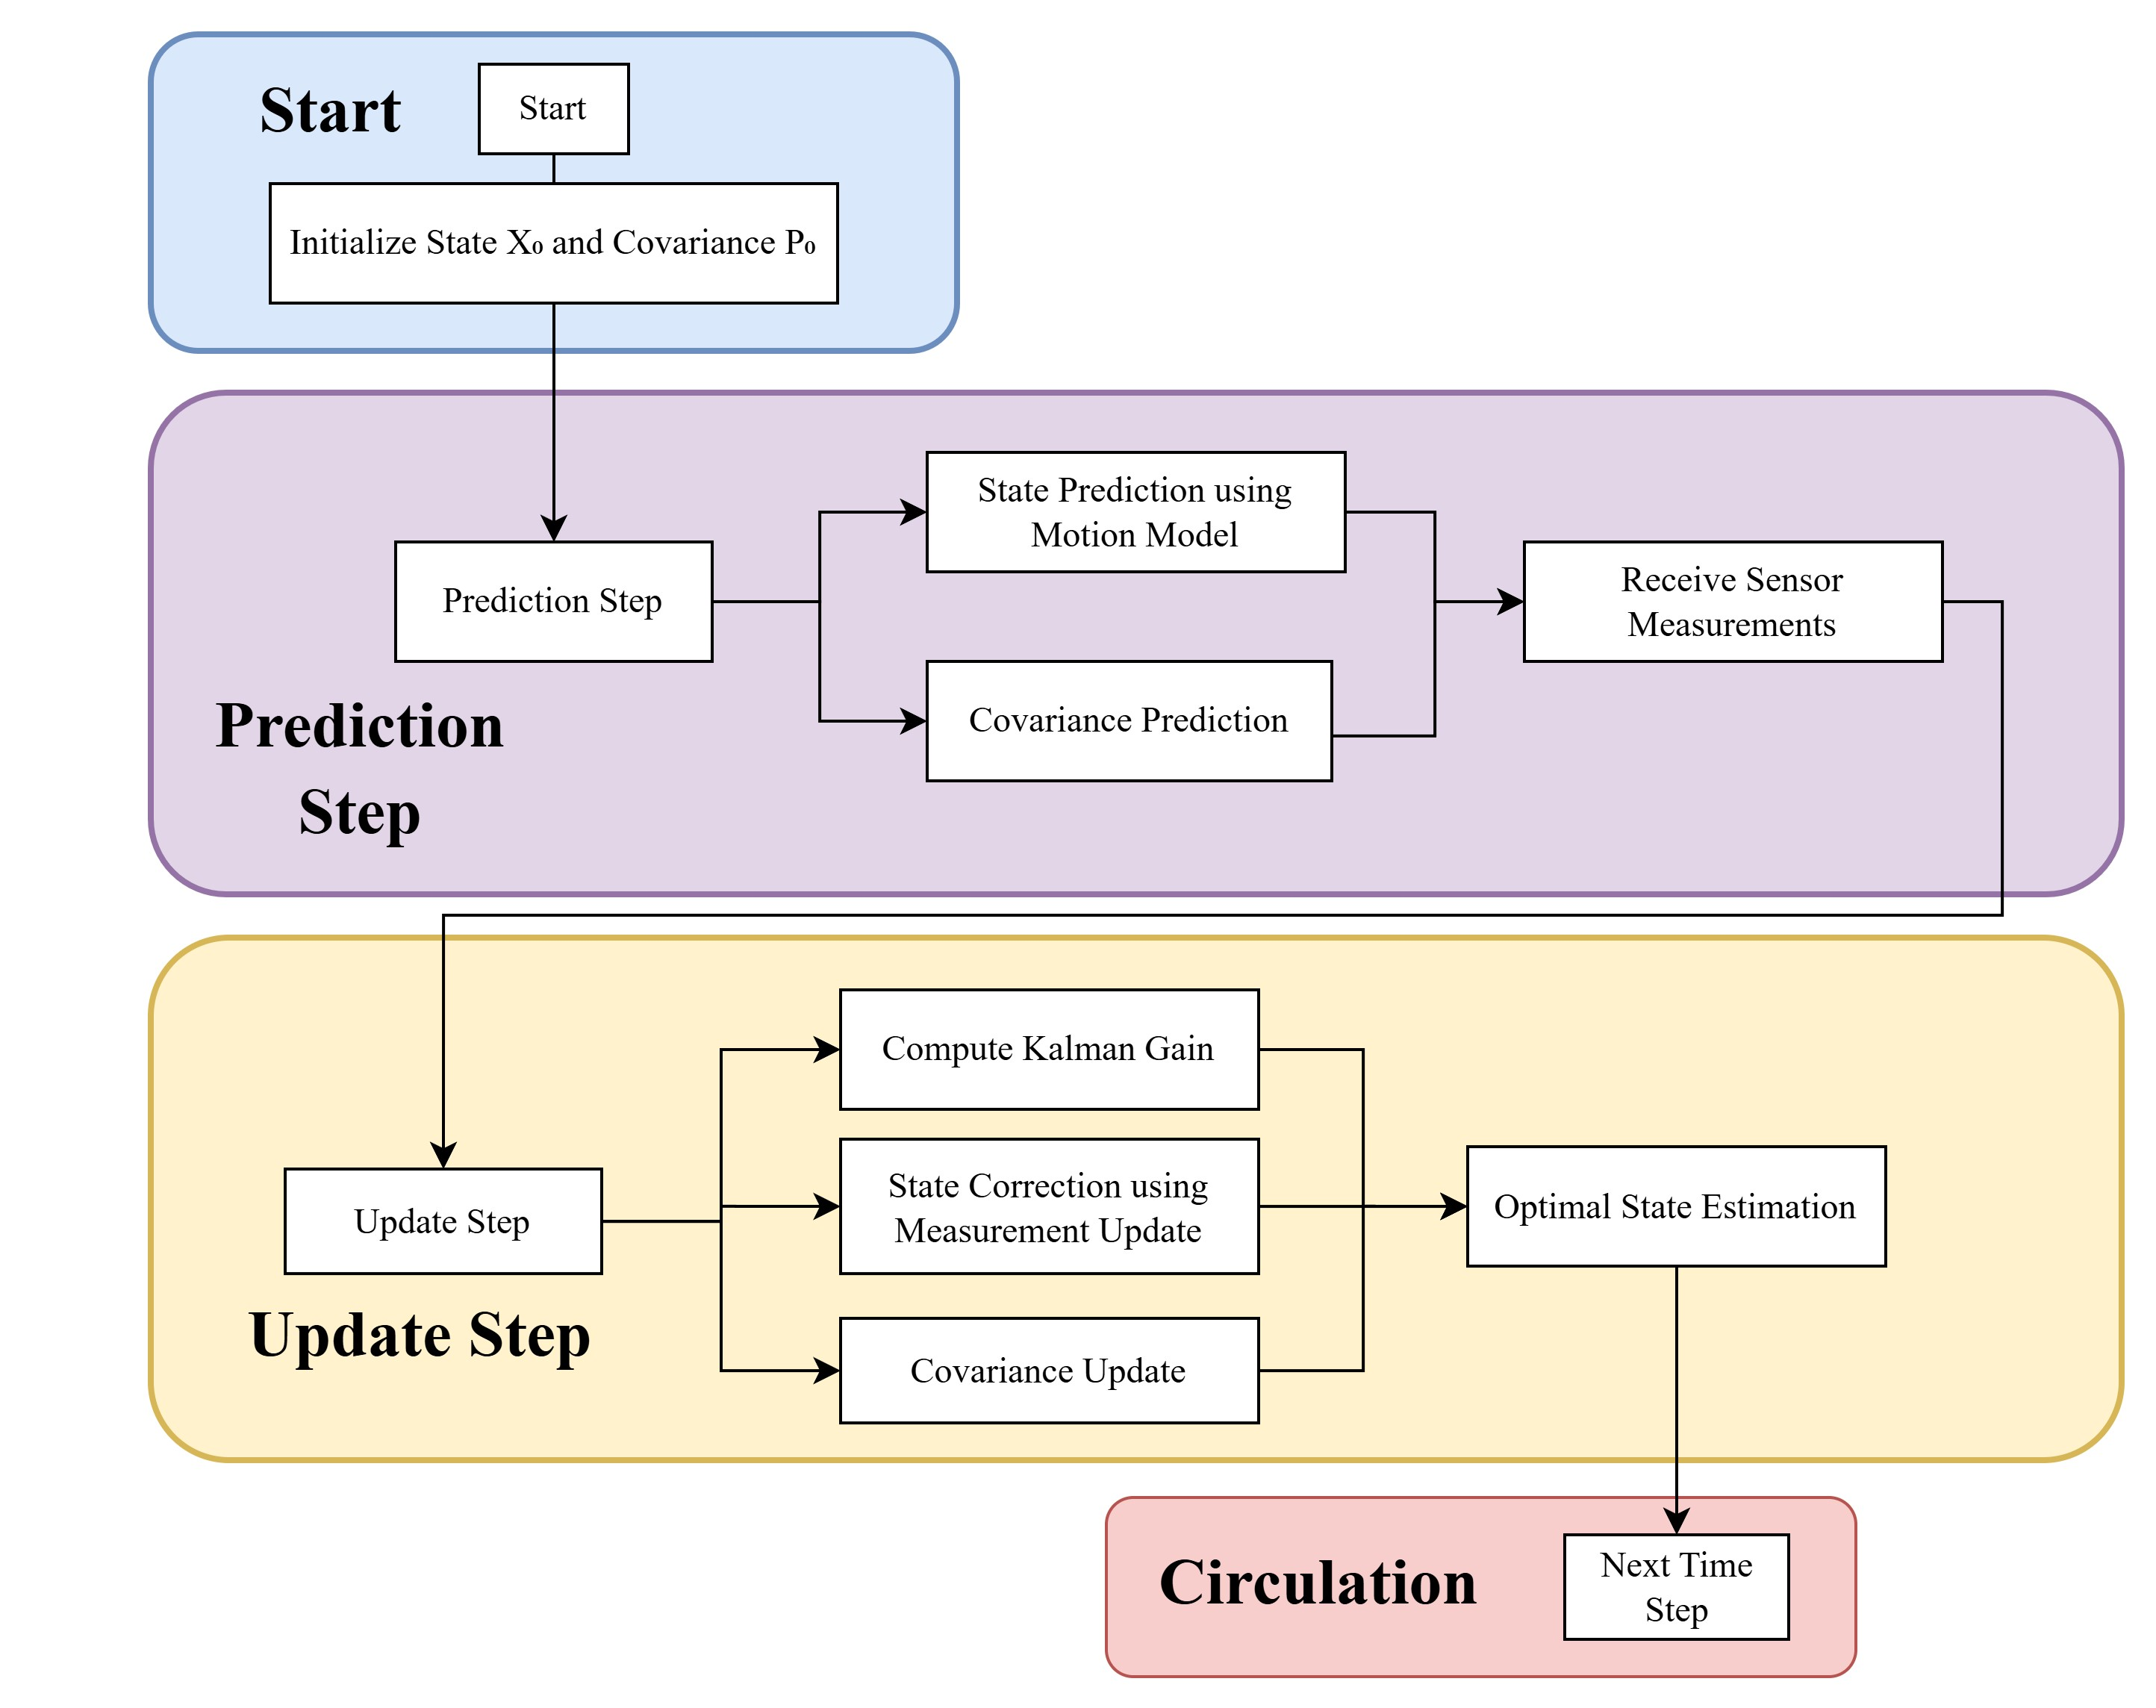
\includegraphics[width=0.85\linewidth]{images/2.jpg}
  \caption{Structural diagram of EKF input and status vector composition.}
  \label{fig:Structural diagram of EKF input and status vector composition}
\end{figure}

Based on the source and characteristics of the perceived information, the system
state is modelled as a nonlinear dynamic process and estimated recursively using
an EKF. The following sections will detail the EKF state modelling method,
including the construction of the system prediction model and observation model,
as well as the role of multi-source observations in the fusion process.

\subsubsection{Prediction Model}
In EKF, the prediction step is used to infer the prior distribution of the
current state based on the state estimate and control input at the previous
moment, and to perform covariance propagation. Let the state vector be
\autoref{eq:Xk_definition}, and the control input $\mathbf{u}_k$ comes from the
IMU sensor, which contains linear acceleration and angular velocity
measurements.
\begin{equation}
  \mathbf{u}_k = 
  \begin{bmatrix}
    a_k \\
    \omega_k
  \end{bmatrix}
  \label{eq:control_input}
\end{equation}
where $\mathbf{u}_k$ denotes the control input vector at time step $k$,
consisting of the measured acceleration and angular velocity from the IMU:
\begin{itemize}
\item $a_k$: the 3D linear acceleration vector, $a_k = [a_x, a_y, a_z]^T$
\item $\omega_k$: the 3D angular velocity vector,
  $\omega_k = [\omega_x, \omega_y, \omega_z]^T$
\end{itemize}

According to the nonlinear kinematic model of the system, the predicted form of
the state at time step $k$ is:
\begin{equation}
  \hat{\mathbf{X}}_{k|k-1} =
  \begin{bmatrix}
    x_{k-1} + v_{k-1} \cdot \Delta t \cdot \cos(\theta_{k-1}) \\
    y_{k-1} + v_{k-1} \cdot \Delta t \cdot \sin(\theta_{k-1}) \\
    \theta_{k-1} + \omega_{k-1} \cdot \Delta t \\
    v_{k-1} + a_k \cdot \Delta t \\
    \omega_k
  \end{bmatrix}
  \label{eq:state_prediction}
\end{equation}
where $\hat{\mathbf{x}}_{k|k-1}$ denotes the predicted state vector at time step
$k$ given information up to time $k{-}1$. The state transition function
incorporates both kinematic and dynamic updates using control
inputs. Specifically:
\begin{itemize}
\item $x_{k-1}, y_{k-1}$: position coordinates at time $k{-}1$
\item $v_{k-1}$: linear velocity at time $k{-}1$
\item $\theta_{k-1}$: heading (yaw) angle at time $k{-}1$
\item $\omega_{k-1}$: angular velocity (yaw rate) at time $k{-}1$
\item $a_k$: linear acceleration at time $k$ (from IMU)
\item $\omega_k$: angular velocity at time $k$ (from IMU)
\item $\Delta t$: discrete time interval
\end{itemize}

The first two rows correspond to position prediction using a constant velocity
motion model; the third row updates the heading angle with angular velocity; the
fourth row propagates linear velocity via acceleration; the final row directly
passes the angular velocity.
\begin{equation}
  \mathbf{F}_k = 
  \begin{bmatrix}
    1 & 0 & -v_k \Delta t \sin(\theta_k) & \Delta t \cos(\theta_k) & 0 \\
    0 & 1 & v_k \Delta t \cos(\theta_k) & \Delta t \sin(\theta_k) & 0 \\
    0 & 0 & 1 & 0 & \Delta t \\
    0 & 0 & 0 & 1 & 0 \\
    0 & 0 & 0 & 0 & 0
  \end{bmatrix}
  \label{eq:jacobian_F}
\end{equation}
where $\mathbf{F}_k$ is the first-order partial derivative of the nonlinear
state transition function $f(\mathbf{x}_k, \mathbf{u}_k)$ with respect to the
state $\mathbf{x}$ (Jacobian matrix), expressed as follows:
\begin{itemize}
\item $v_k$: the current linear velocity of the robot (obtained from the control
  input or state variables)
\item $\theta_k$: the robot's current heading angle
\item $\Delta t$: discrete time interval
\end{itemize}

Note that the first two columns of $\mathbf{F}_k$ are constant because the
position components $x$ and $y$ are not directly influenced by themselves in the
transition function, but rather updated through the control variables $v_k$ and
$\theta_k$. Therefore, $\partial x_{k+1} / \partial x_k = 1$ and
$\partial y_{k+1} / \partial y_k = 1$, resulting in identity entries in the
upper-left block of the Jacobian.

This matrix is the state transition Jacobian of the linearized state transition
function $f(\mathbf{x}_k)$, used to predict state covariance.  The covariance
propagation formula is:
\begin{equation}
  \mathbf{P}_{k|k-1} = \mathbf{F}_k \mathbf{P}_{k-1} \mathbf{F}_k^\top + \mathbf{Q}_k
  \label{eq:cov_prediction}
\end{equation}
where $\mathbf{P}_{k-1}$ is the state covariance from the previous step, and
$\mathbf{Q}_k$ is the process noise covariance matrix. This prediction stage
provides a dynamic prior estimate of the current state of the system, which
serves as the basis for subsequent observation updates.

\subsubsection{Update Model}
After completing state prediction, the EKF enters the observation update phase,
which introduces actual observation information from external sensors (such as
SLAM or Wi-Fi) into the system state estimation. The core objective of this
process is to correct the predicted state based on the current observations,
thereby reducing the cumulative deviation caused by system modelling errors or
process noise. Let the observation result of the sensor at time step $k$ be
$z_k$, and the corresponding observation model be:
\begin{equation}
  \mathbf{z}_k = h(\mathbf{X}_k) + \mathbf{v}_k =
  \begin{bmatrix}
    x_k \\
    y_k
  \end{bmatrix} + \mathbf{v}_k
  \label{eq:observation_model}
\end{equation}
where \(\mathbf{z}_k \in \mathbb{R}^2\) represents a two-dimensional real-valued
vector, consists of position observations from either the Wi-Fi fingerprint
module or the SLAM system. $h(\mathbf{X}_k)$ is a nonlinear observation
function, $\mathbf{v}_k$ is zero-mean Gaussian noise with covariance $R_k$. In
this study, we assume that the observations are the positions of the platform on
a two-dimensional map, so the observation function is:
\begin{equation}
  h(\mathbf{X}_k) = 
  \begin{bmatrix}
    x_k \\
    y_k
  \end{bmatrix}
\end{equation}
\noindent
where $h(\mathbf{X}_k)$ denotes the observation model that maps the full state
vector $\mathbf{X}_k$ to the measurable output. In this case:
\begin{itemize}
\item $\mathbf{X}_k$: the full state vector at time $k$, typically including
  position, orientation, velocity, etc.
\item $x_k, y_k$: the 2D position coordinates extracted from the state for
  observation.
\end{itemize}

The Jacobian matrix of the observation model $\mathbf{H}_k$ is a constant matrix
\begin{equation}
  \mathbf{H}_k = \frac{\partial h}{\partial \mathbf{X}_k}
\end{equation}
where $\mathbf{H}_k$ is the Jacobian matrix of the observation function
$h(\mathbf{X}_k)$ with respect to the state vector $\mathbf{X}_k$, evaluated at
time step $k$. It describes the sensitivity of the observable outputs to small
changes in the system state. In the case where $h(\mathbf{X}_k) = [x_k, y_k]^T$
and $\mathbf{X}_k = [x_k, y_k, \theta_k, v_k, \omega_k]^T$, the matrix
$\mathbf{H}_k$ takes the following form:
\[
  \mathbf{H}_k =
  \begin{bmatrix}
    1 & 0 & 0 & 0 & 0 \\
    0 & 1 & 0 & 0 & 0
  \end{bmatrix}
\]
After obtaining the predicted state \(\hat{\mathbf{X}}_{k|k-1}\) and the
predicted covariance \(\mathbf{P}_{k|k-1}\), the system first calculates the
Kalman gain.
\begin{equation}
  \mathbf{K}_k = \mathbf{P}_{k|k-1} \mathbf{H}_k^\top 
  \left( \mathbf{H}_k \mathbf{P}_{k|k-1} \mathbf{H}_k^\top + \mathbf{R}_k \right)^{-1}
  \label{eq:kalman_gain}
\end{equation}
where $\mathbf{K}_k$ is the Kalman gain matrix at time step $k$, determining how
much the predicted state should be corrected based on the new
observation. Specifically:
\begin{itemize}
\item $\mathbf{P}_{k|k-1}$: the predicted error covariance matrix before the
  update step
\item $\mathbf{H}_k$: the observation model Jacobian matrix at time $k$
\item $\mathbf{R}_k$: the observation noise covariance matrix
\end{itemize}

The gain matrix is used to balance prediction uncertainty and observation noise,
determining the magnitude of the final state correction. Subsequently, the state
vector is updated based on the observation residual
\begin{equation}
  \hat{\mathbf{X}}_k = \hat{\mathbf{X}}_{k|k-1} + \mathbf{K}_k 
  \left( \mathbf{z}_k - h(\hat{\mathbf{X}}_{k|k-1}) \right)
  \label{eq:state_update}
\end{equation}
where $\hat{\mathbf{x}}_k$ is the updated state estimate at time $k$ after
incorporating the measurement. The correction term
$\mathbf{K}_k \left( \mathbf{z}_k - h(\hat{\mathbf{x}}_{k|k-1}) \right)$ adjusts
the prediction based on the innovation (residual) between the actual observation
and the predicted observation. Specifically:
\begin{itemize}
\item $\hat{\mathbf{x}}_{k|k-1}$: the predicted state before the measurement
  update
\item $\mathbf{K}_k$: the Kalman gain at time $k$
\item $\mathbf{z}_k$: the actual observation (measurement vector)
\item $h(\hat{\mathbf{x}}_{k|k-1})$: the predicted observation derived from the
  predicted state
\end{itemize}

This update rule ensures that the new estimate $\hat{\mathbf{x}}_k$ is a
weighted combination of the prior prediction and the new measurement, accounting
for their respective uncertainties.

Finally, the system synchronizes and corrects the state covariance matrix to
reflect the updated uncertainty distribution.
\begin{equation}
  \mathbf{P}_k = (\mathbf{I} - \mathbf{K}_k \mathbf{H}_k) \mathbf{P}_{k|k-1}
  \label{eq:cov_update}
\end{equation}
\noindent
where $\mathbf{P}_k$ is the updated error covariance matrix at time step $k$. It
reflects the uncertainty associated with the updated state
estimate. Specifically:
\begin{itemize}
  \item $\mathbf{I}$: the identity matrix of appropriate dimensions
\end{itemize}

Through the above update steps, EKF can dynamically correct the platform status
at each observation time, thereby achieving effective fusion of multi-source
information and continuous improvement in state estimation accuracy.

Ultimately, the system can output continuous, smooth, and accurate position and
attitude estimation results in real time in complex dynamic environments,
achieving an organic integration of the global consistency provided by Wi-Fi and
the local high-frequency dynamic perception of IMU, significantly enhancing the
robustness and stability of the localization system under sensor uncertainty and
environmental disturbances.

\subsubsection{Performance evaluation}
After completing the EKF fusion, we obtained the trajectory map after Wi-Fi,
IMU, and SLAM data fusion using EKF. To further enhance the reliability of the
experimental results and quantify the accuracy of the localization system after
the fusion of different sensor data, this study introduced the mean squared
error (MSE) and mean absolute error (MAE) as performance evaluation
indicators. These two indicators reflect the accuracy and robustness of the
localization system from different perspectives, thereby providing strong
quantitative support for the effectiveness of multi-source data fusion.

MSE and MAE are widely used error evaluation standards in current indoor
localization research, especially suitable for fingerprint localization and
multi-sensor fusion scenarios, and have been widely verified by multiple studies
for their effectiveness and universality~\cite{sun2019fusion, he2015wi}.
\begin{equation}
  \text{MSE} = \frac{1}{N} \sum_{i=1}^{N} \left( x_{\text{true}, i} - x_{\text{pred}, i} \right)^2 + \left( y_{\text{true}, i} - y_{\text{pred}, i} \right)^2
  \label{MSE}
\end{equation}
where, $N$ is the number of test data points, $x_{\text{true}, i}$ and
$y_{\text{true}, i}$ are the actual location coordinates of the $i_{th}$ test
point, and $x_{\text{pred}, i}$ and $y_{\text{pred}, i}$ are the coordinates
predicted by Wi-Fi, IMU, or EKF.  The mean absolute error is used to measure the
absolute magnitude of the difference between the predicted value and the actual
value. Compared with MSE, MAE is less sensitive to outliers and can more clearly
reflect the overall accuracy of the model.
\begin{equation}
  \text{MAE} = \frac{1}{N} \sum_{i=1}^{N} \left| x_{\text{true}, i} - x_{\text{pred}, i} \right| + \left| y_{\text{true}, i} - y_{\text{pred}, i} \right|
  \label{MAE}
\end{equation}
where $\left| \,\cdot\, \right|$ denotes absolute value, and the meanings of
other symbols are consistent with those in~\autoref{MSE}.

After calculating the error of the entire trajectory, in order to further
analyse the localization accuracy of the system at certain moments, we also used
a local magnification to show the specific situation at the point of maximum
error. By magnifying the displayed area, we can clearly see the error between
Wi-Fi and IMU and EKF, and further compare the performance of different sensors
at specific locations, especially in areas where Wi-Fi localization errors are
significant. In order to quantitatively evaluate these errors, we used the
following error calculation formula:
\begin{equation}
  \text{Wi-Fi Error} = \sqrt{(x_{\text{EKF}}(t) - x_{\text{WiFi}}(t))^2 + (y_{\text{EKF}}(t) - y_{\text{WiFi}}(t))^2}
\end{equation}

\begin{equation}
  \text{IMU Error} = \sqrt{(x_{\text{EKF}}(t) - x_{\text{IMU}}(t))^2 + (y_{\text{EKF}}(t) - y_{\text{IMU}}(t))^2}
\end{equation}
where \( x_{\text{EKF}}(t), y_{\text{EKF}}(t) \) denote the 2D location
estimated by EKF, and \( x_{\text{WiFi}}(t), y_{\text{WiFi}}(t) \) and \(
x_{\text{IMU}}(t), y_{\text{IMU}}(t) \) denote the predicted location from Wi-Fi
and IMU.

By using Euclidean distance for intuitive visualization, we can better
understand changes in system accuracy and verify the advantages of EKF in
complex environments.


\newpage
\section{Experimental Results}
All experiments in this study were conducted on a mobile AGV platform equipped
with NVIDIA Jetson computing modules, 2D LiDAR, an inertial measurement unit
(IMU), and a Wi-Fi receiver, as shown in~\autoref{fig:Hardware platform
  components of AGV}

\subsection{Multi-floor comparison under similar indoor settings}
To validate the proposed EKF-based multi-source fusion localization framework,
this study conducted a series of indoor localization experiments on the 6th,
7th, and 8th floors of the IR building at Xi'an Jiaotong-Liverpool
University. The experiments were mainly conducted in the corridor areas of the
floors, taking into account factors such as signal obstruction and dynamic
movement in the environment to test the localization accuracy and stability of
the system in complex environments.

During the experiments, the platform followed a predefined trajectory while
simultaneously collecting Wi-Fi RSSI, IMU, and LiDAR data. Wi-Fi data was
processed through a DNN model for regression, utilizing the RSSI vectors of each
reference point for training to predict the corresponding location. This study
set up three localization schemes for comparison:
\begin{itemize}
\item Using only the Wi-Fi fingerprint regression model
\item Using only IMU inertial measurements
\item Using EKF for localization results after Wi-Fi, IMU, and SLAM data fusion
\end{itemize}
\begin{figure}[H]
  \centering
  \includegraphics[width=0.9\linewidth]{images/IR_half_circle.png}
  \caption{First phase indoor localization experimental path.}
  \label{fig:First phase indoor localization experimental path}
\end{figure}

The first phase of the experiment was conducted in similar corridor areas on the
6th, 7th, and 8th floors of the IR building. To ensure a comprehensive
evaluation of the performance of different sensors, we conducted experiments in
the same areas across the three floors (as shown in~\autoref{fig:First phase
  indoor localization experimental path}), obtaining three sets of path maps
that demonstrate the experimental results for the three floors. Each set of
graphs shows the trajectories of Wi-Fi localization, IMU localization, and EKF
fusion localization, which are distinguished by different colours and line
types. The blue trajectory represents the results after EKF fusion, the orange
dotted line represents Wi-Fi localization, and the green dotted line represents
IMU localization results\nomenclature{MAE}{Mean Absolute Error}.

As shown in~\autoref{fig:Comparison of experimental trajectories on the 7th
  floor}, the trajectories obtained using the Wi-Fi, IMU, and EKF fusion method
are displayed. In the Wi-Fi localization results, due to the influence of signal
obstruction and reflection in the environment, the localization trajectory
showed apparent deviations, indicating that Wi-Fi localization is susceptible to
multipath propagation and signal attenuation in indoor environments. The IMU
localization results showed significant errors, especially when the platform was
moving quickly or turning, as the IMU system errors tended to accumulate,
leading to a decrease in localization accuracy. In contrast, the EKF fusion
method effectively combines the data advantages of Wi-Fi and IMU, providing
smoother and more accurate trajectories through multiple corrections of state
estimates and sensor data.
\begin{figure}[H]
  \centering
  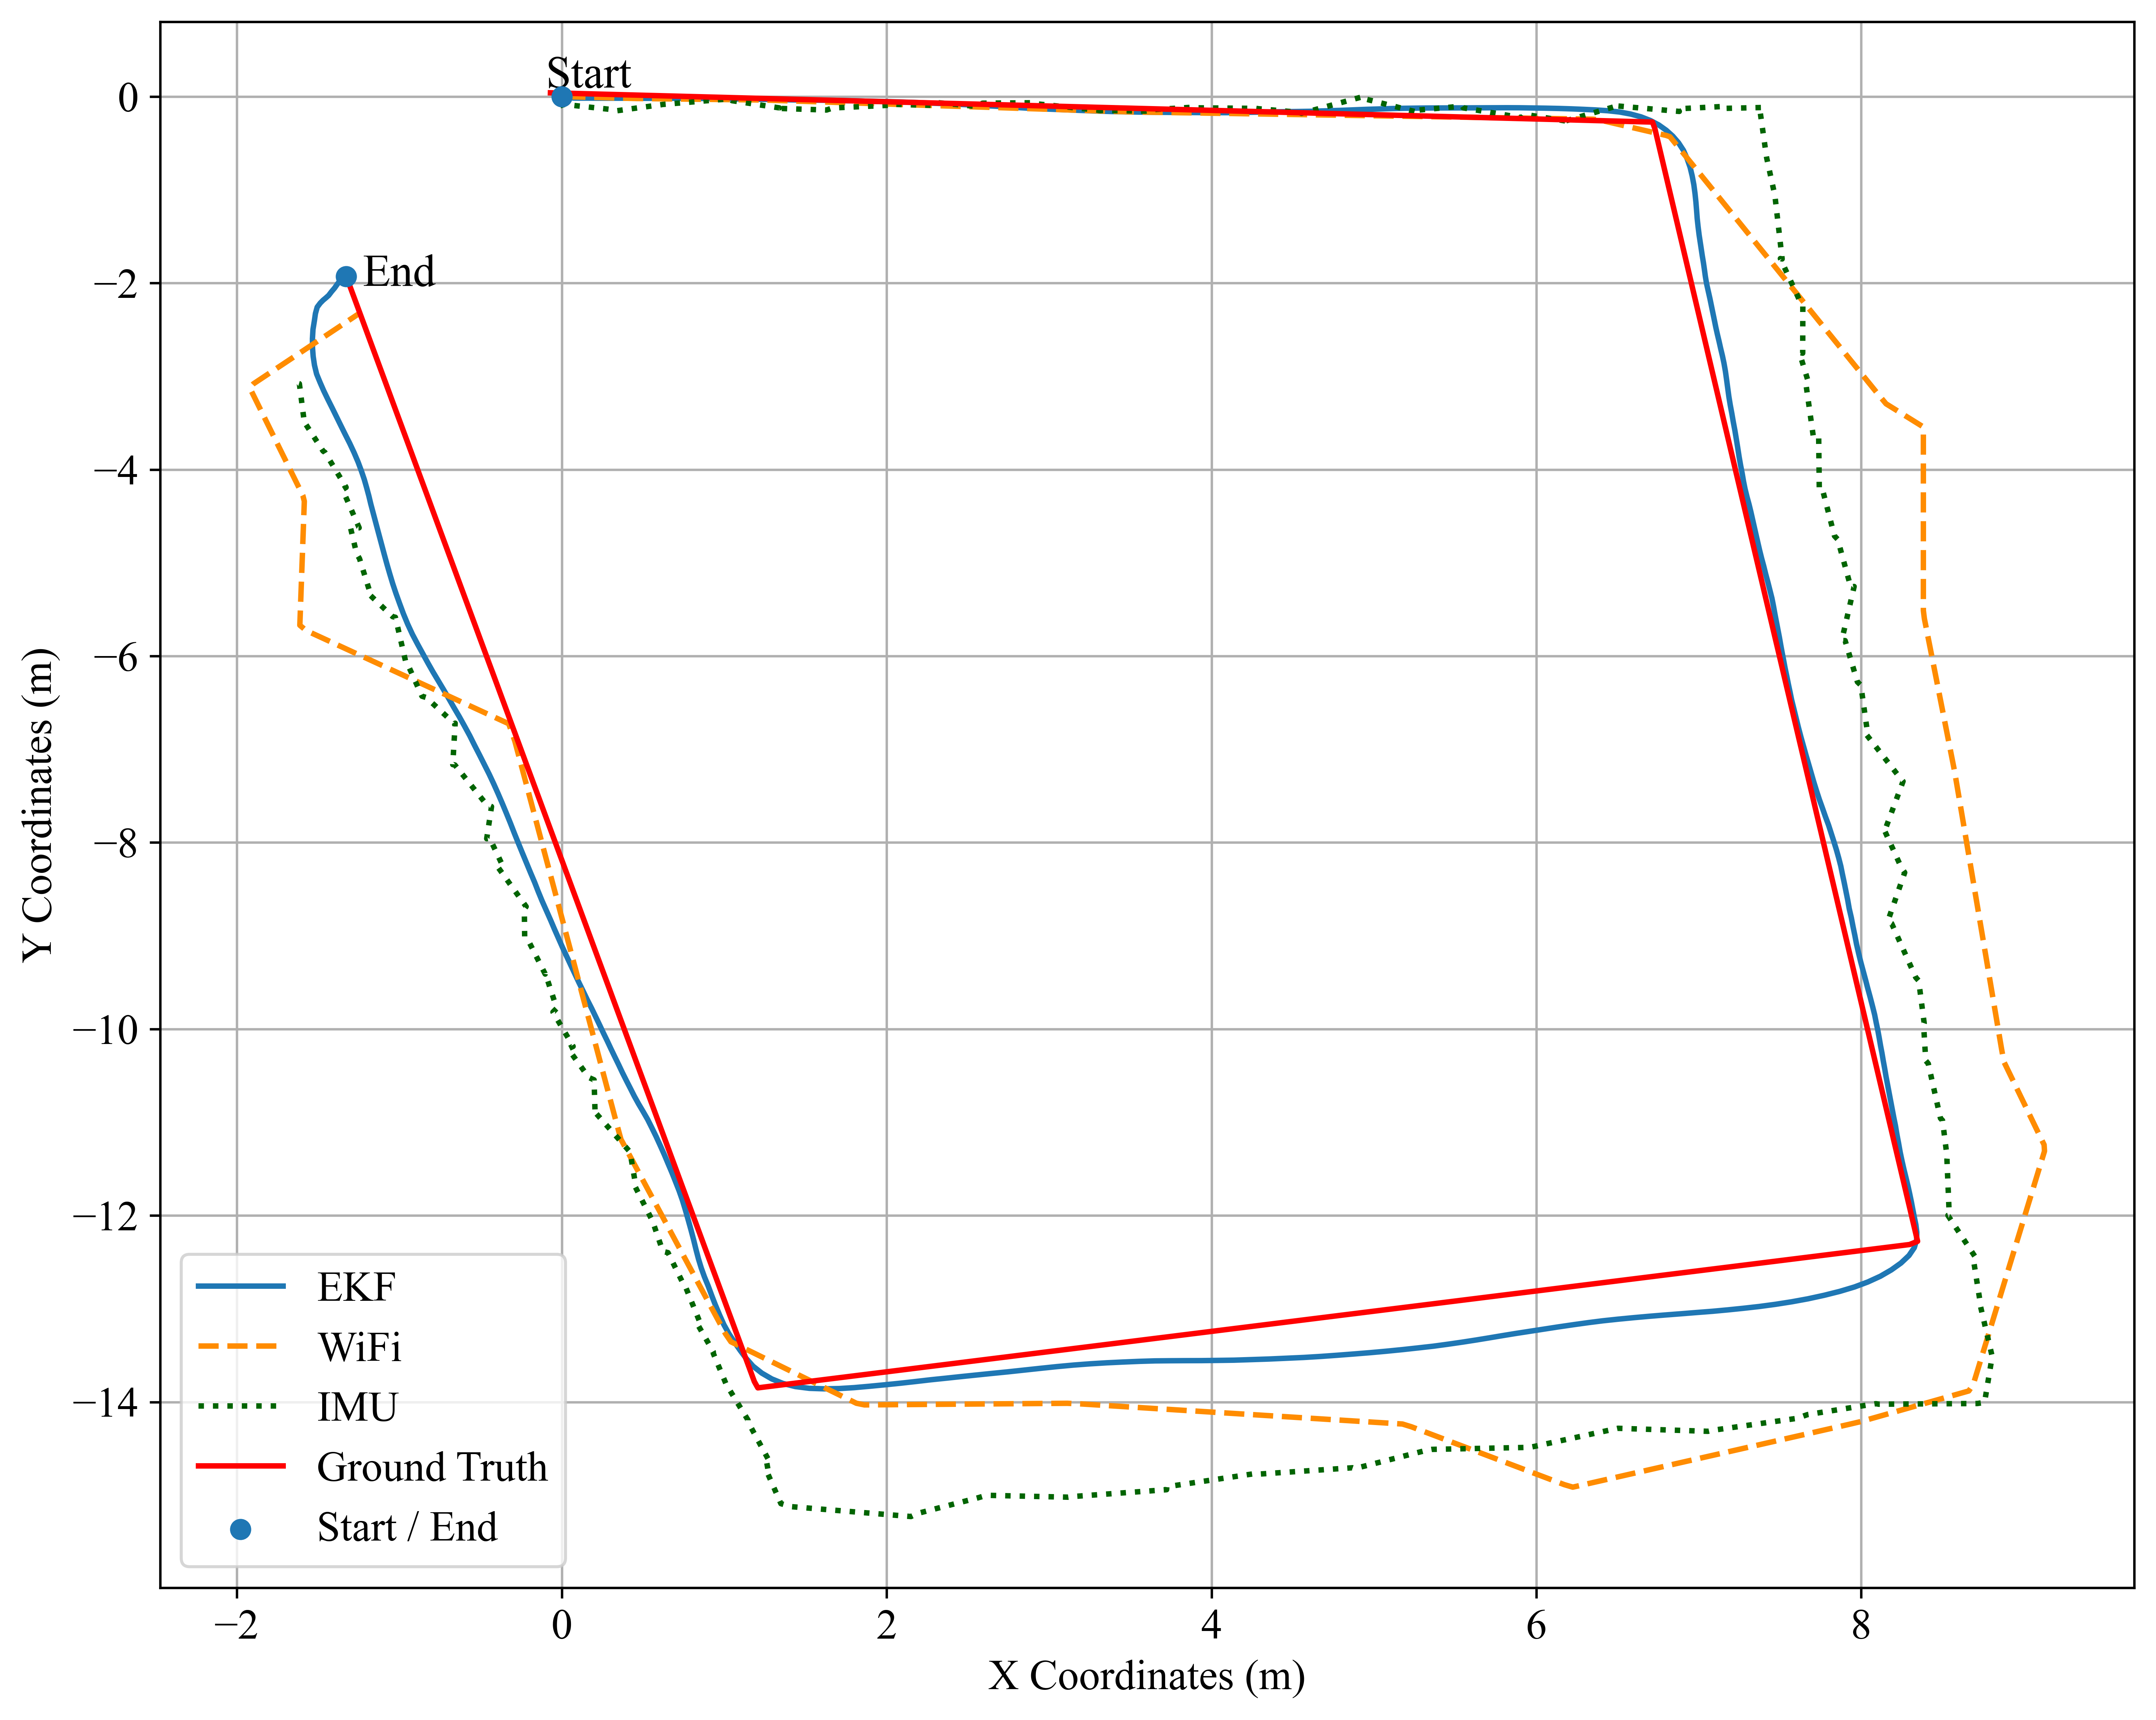
\includegraphics[width=0.7\linewidth]{images/1/2.png}
  \caption{Comparison of experimental trajectories on the 7th floor.}
  \label{fig:Comparison of experimental trajectories on the 7th floor}
\end{figure}

\autoref{tab:7th_floor_accuracy} shows the MSE and MAE calculated for this
experiment relative to the EKF fusion method. For Wi-Fi localization, the
experimental results show that the MAE of Wi-Fi is 1.1159 and the MSE is 1.9694,
indicating that compared to EKF, Wi-Fi localization has a larger deviation and
fluctuation in estimating spatial coordinates. The MAE of IMU localization is
0.9208, and the MSE is 1.8722, showing that IMU can provide relatively stable
motion estimates in a short period of time. However, in long-term localization
tasks, the error is still large, especially in rapidly changing environments.
\begin{table}[H]
  \centering
  \caption{7th floor localization accuracy evaluation}
  \label{tab:7th_floor_accuracy}
  \begin{tabular}{lcc}
    \toprule
    \textbf{Localization Method} & \textbf{MAE (m)} & \textbf{MSE (m$^2$)} \\
    \midrule
    Wi-Fi (w.r.t EKF) & 1.1159 & 1.9694 \\
    IMU (w.r.t EKF)   & 0.9208 & 1.8722 \\
    EKF (w.r.t Ground Truth)    & 0.5690 & 0.9070 \\
    \bottomrule
  \end{tabular}
\end{table}

As shown in~\autoref{fig:Error amplification diagram 7th}, the maximum error of
Wi-Fi localization and EKF fusion localization at a certain moment is
displayed. Through the local magnification, we can see that the maximum Wi-Fi
localization error mainly occurs in areas where signal attenuation and multipath
effects are significant, which causes a large deviation in Wi-Fi localization.
\begin{figure}[H]
  \centering
  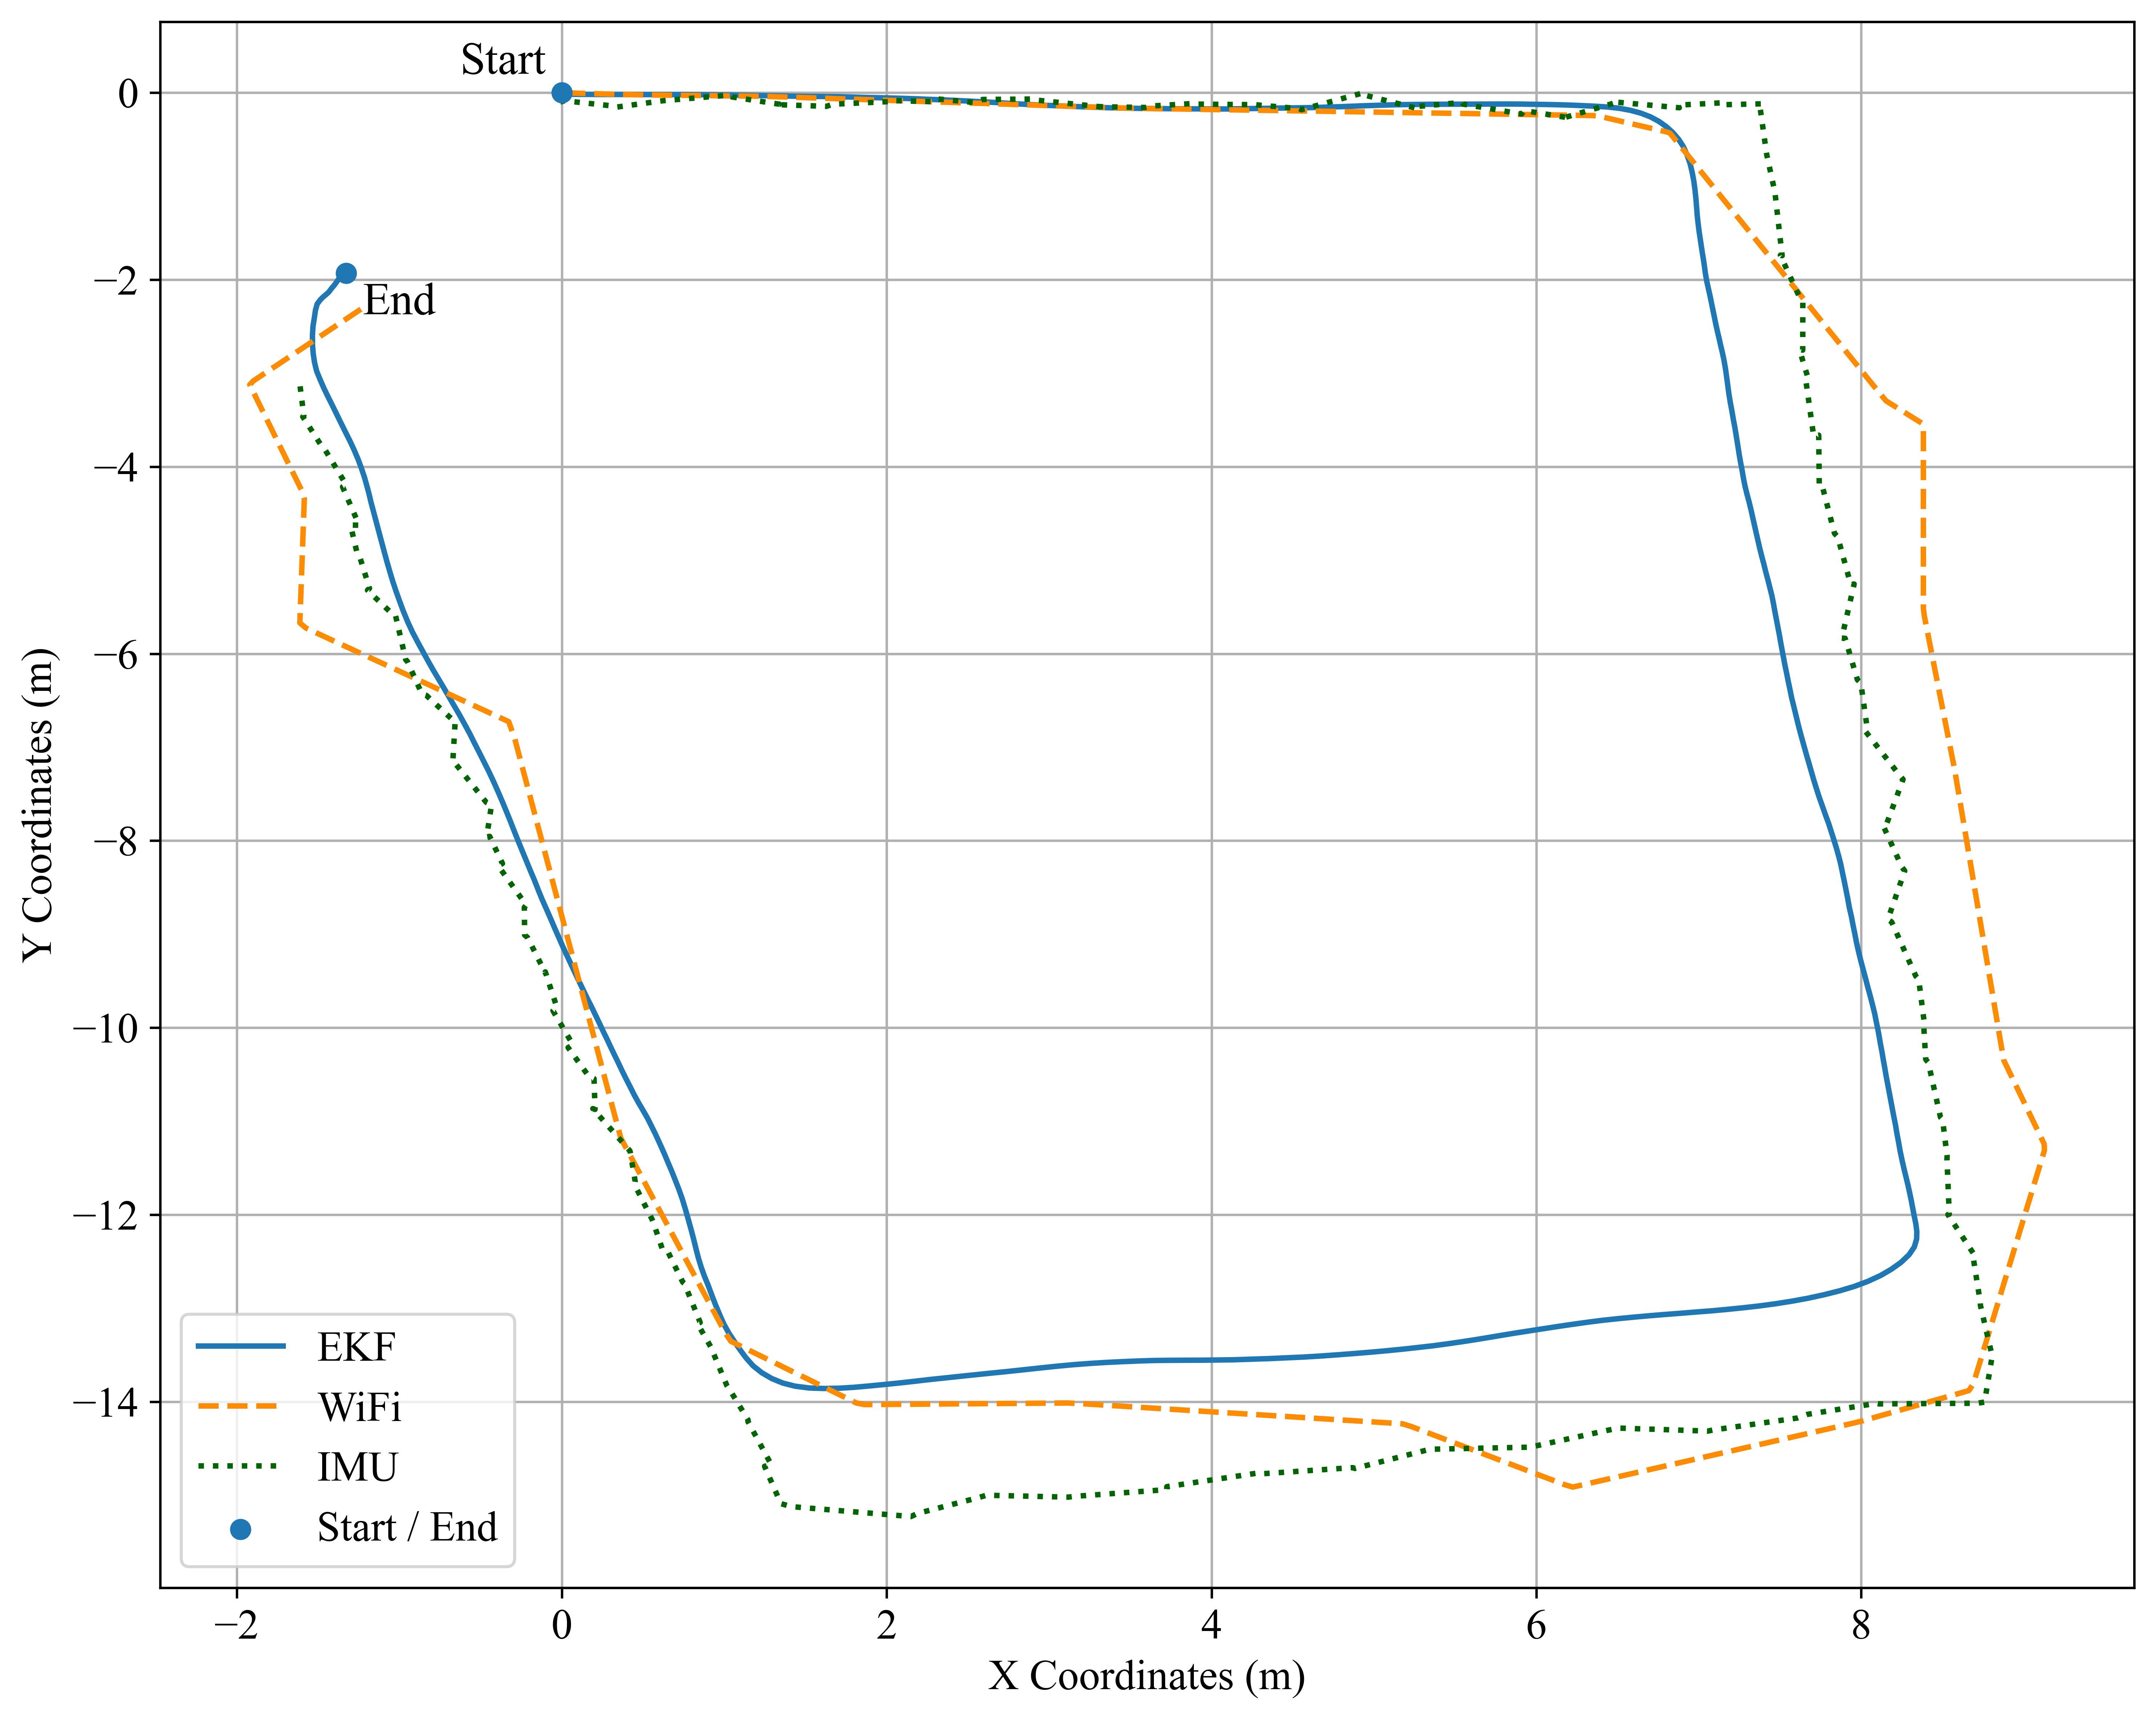
\includegraphics[width=1\linewidth]{Amplification
    images/wifi/half_circle_large_diff.png}
  \caption{Amplified image of the error in the comparison of the experimental
    trajectories on the 7th floor.}
  \label{fig:Error amplification diagram 7th}
\end{figure}

The following section presents the results of the experiment conducted on the
6th floor of the IR Building. Similar to the experiment on the 7th floor, this
experiment compared the localization accuracy of different sensors and EKF under
the same path conditions in this environment to evaluate the performance of
different sensors and fusion methods in this environment.
\begin{figure}[H]
  \centering
  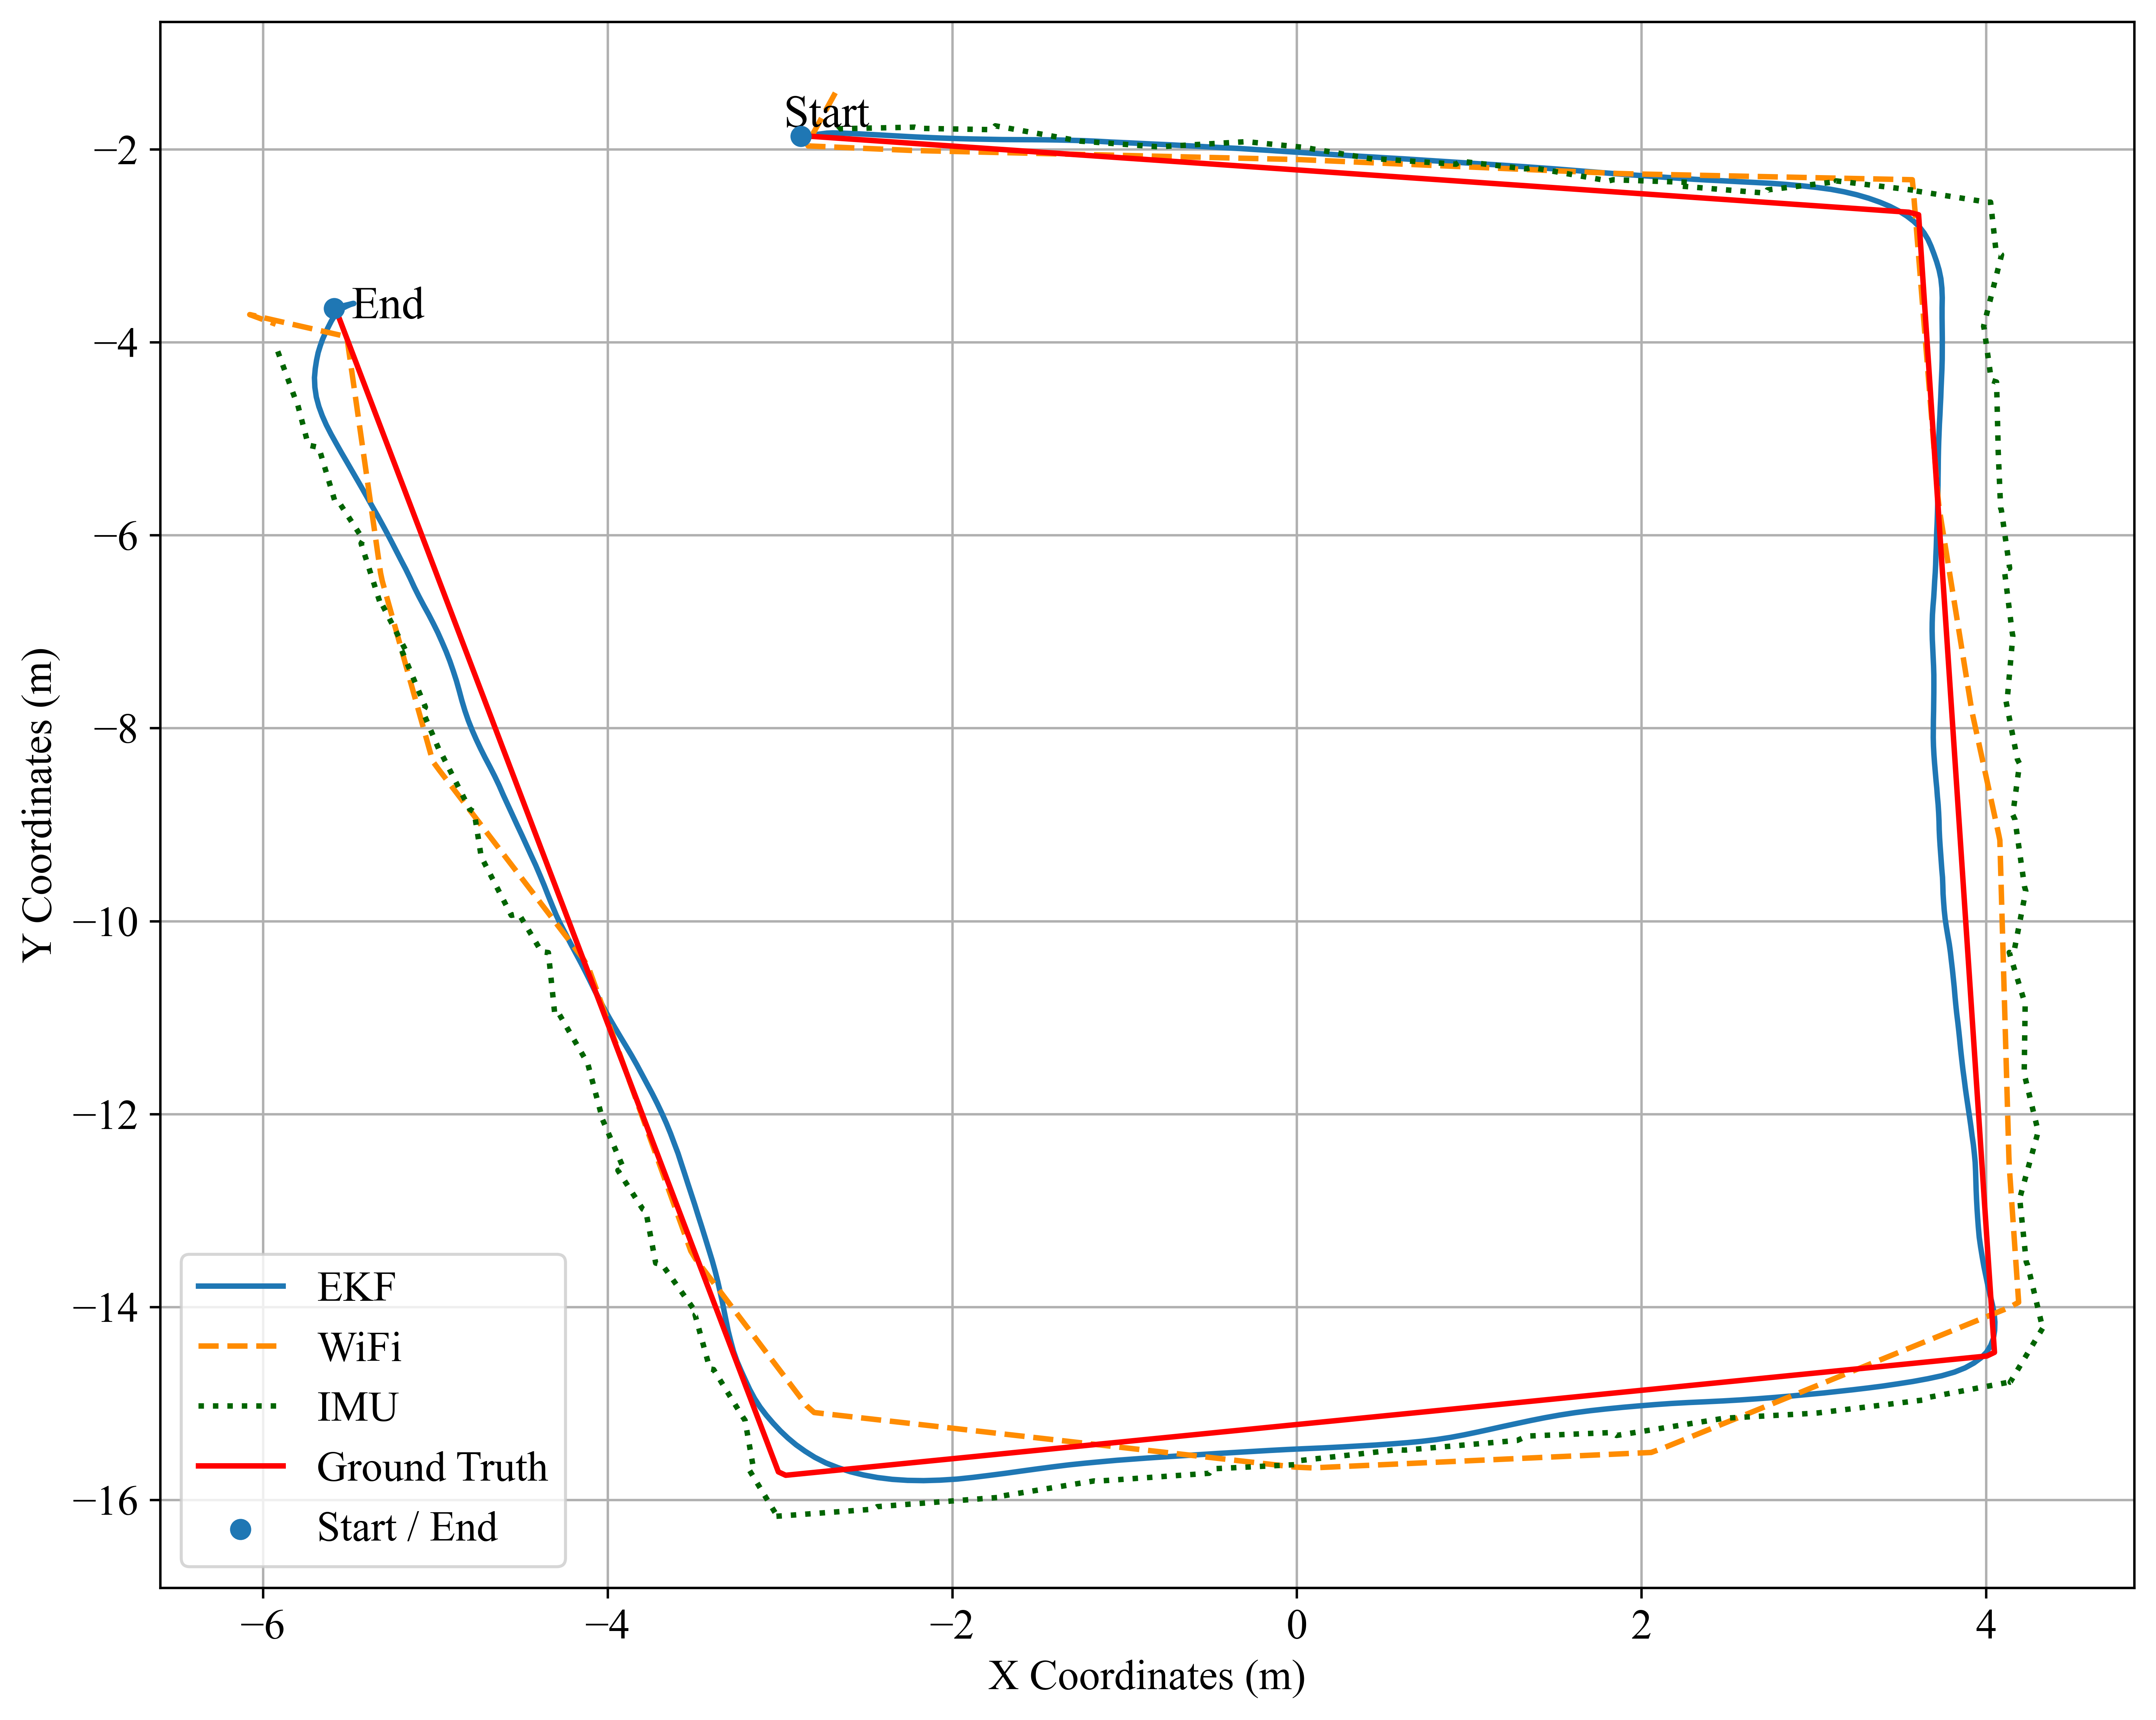
\includegraphics[width=0.7\linewidth]{images/1/4.png}
  \caption{Comparison of experimental trajectories on the 6th floor.}
  \label{fig:Comparison of experimental trajectories on the 6th floor}
\end{figure}

As can be seen from~\autoref{fig:Comparison of experimental trajectories on the
  6th floor}, the trajectory results obtained on the 6th floor of the IR
building are similar to the experimental results on the 7th floor. The drift of
the Wi-Fi localization trajectory is relatively small, but due to signal
frequency limitations, the trajectory still exhibits some smoothness issues. IMU
localization showed a significant decrease in localization accuracy when turning
corners. The EKF method effectively combines the advantages of Wi-Fi and IMU to
provide a smoother and more accurate trajectory.

\autoref{tab:accuracy_evaluation_6th_floor} shows that in the experiment on the
sixth floor, the accuracy of Wi-Fi localization was significantly improved
compared with the test results on the seventh floor. Specifically, the MSE of
Wi-Fi decreased from 1.9694 to 0.0855, and the MAE decreased from 1.1159 to
0.2335. In contrast, the localization accuracy of IMU did not change
significantly, with MAE of 0.8801 and MSE of 1.7431.
\begin{table}[htbp]
  \centering
  \caption{6th floor localization accuracy evaluation (MAE and MSE)}
  \label{tab:accuracy_evaluation_6th_floor} % Add label for reference
  \begin{tabular}{lcc}
    \toprule
    \textbf{Localization Method} & \textbf{MAE (m)} & \textbf{MSE (m$^2$)} \\
    \midrule

    Wi-Fi (w.r.t EKF)                       & 0.2335                             & 0.0855                             \\ 
    IMU (w.r.t EKF)                           & 0.8801                             & 1.7431                             \\ 
    EKF (w.r.t Ground Truth) & 0.697 & 1.144 \\
    \bottomrule
  \end{tabular}
\end{table}

In addition, in order to analyze the specific situation of error distribution,
the local enlarged view shown in~\autoref{fig:Error amplification diagram 6th}
clearly shows the maximum error between Wi-Fi and EKF at certain
moments. Through the local enlarged display, we can see that although the
accuracy of Wi-Fi localization has been significantly improved, there are still
errors between Wi-Fi and EKF. This further verifies that the EKF method can
effectively fuse different sensor data in complex environments and provide more
accurate and stable localization results.
\begin{figure}[H]
  \centering
  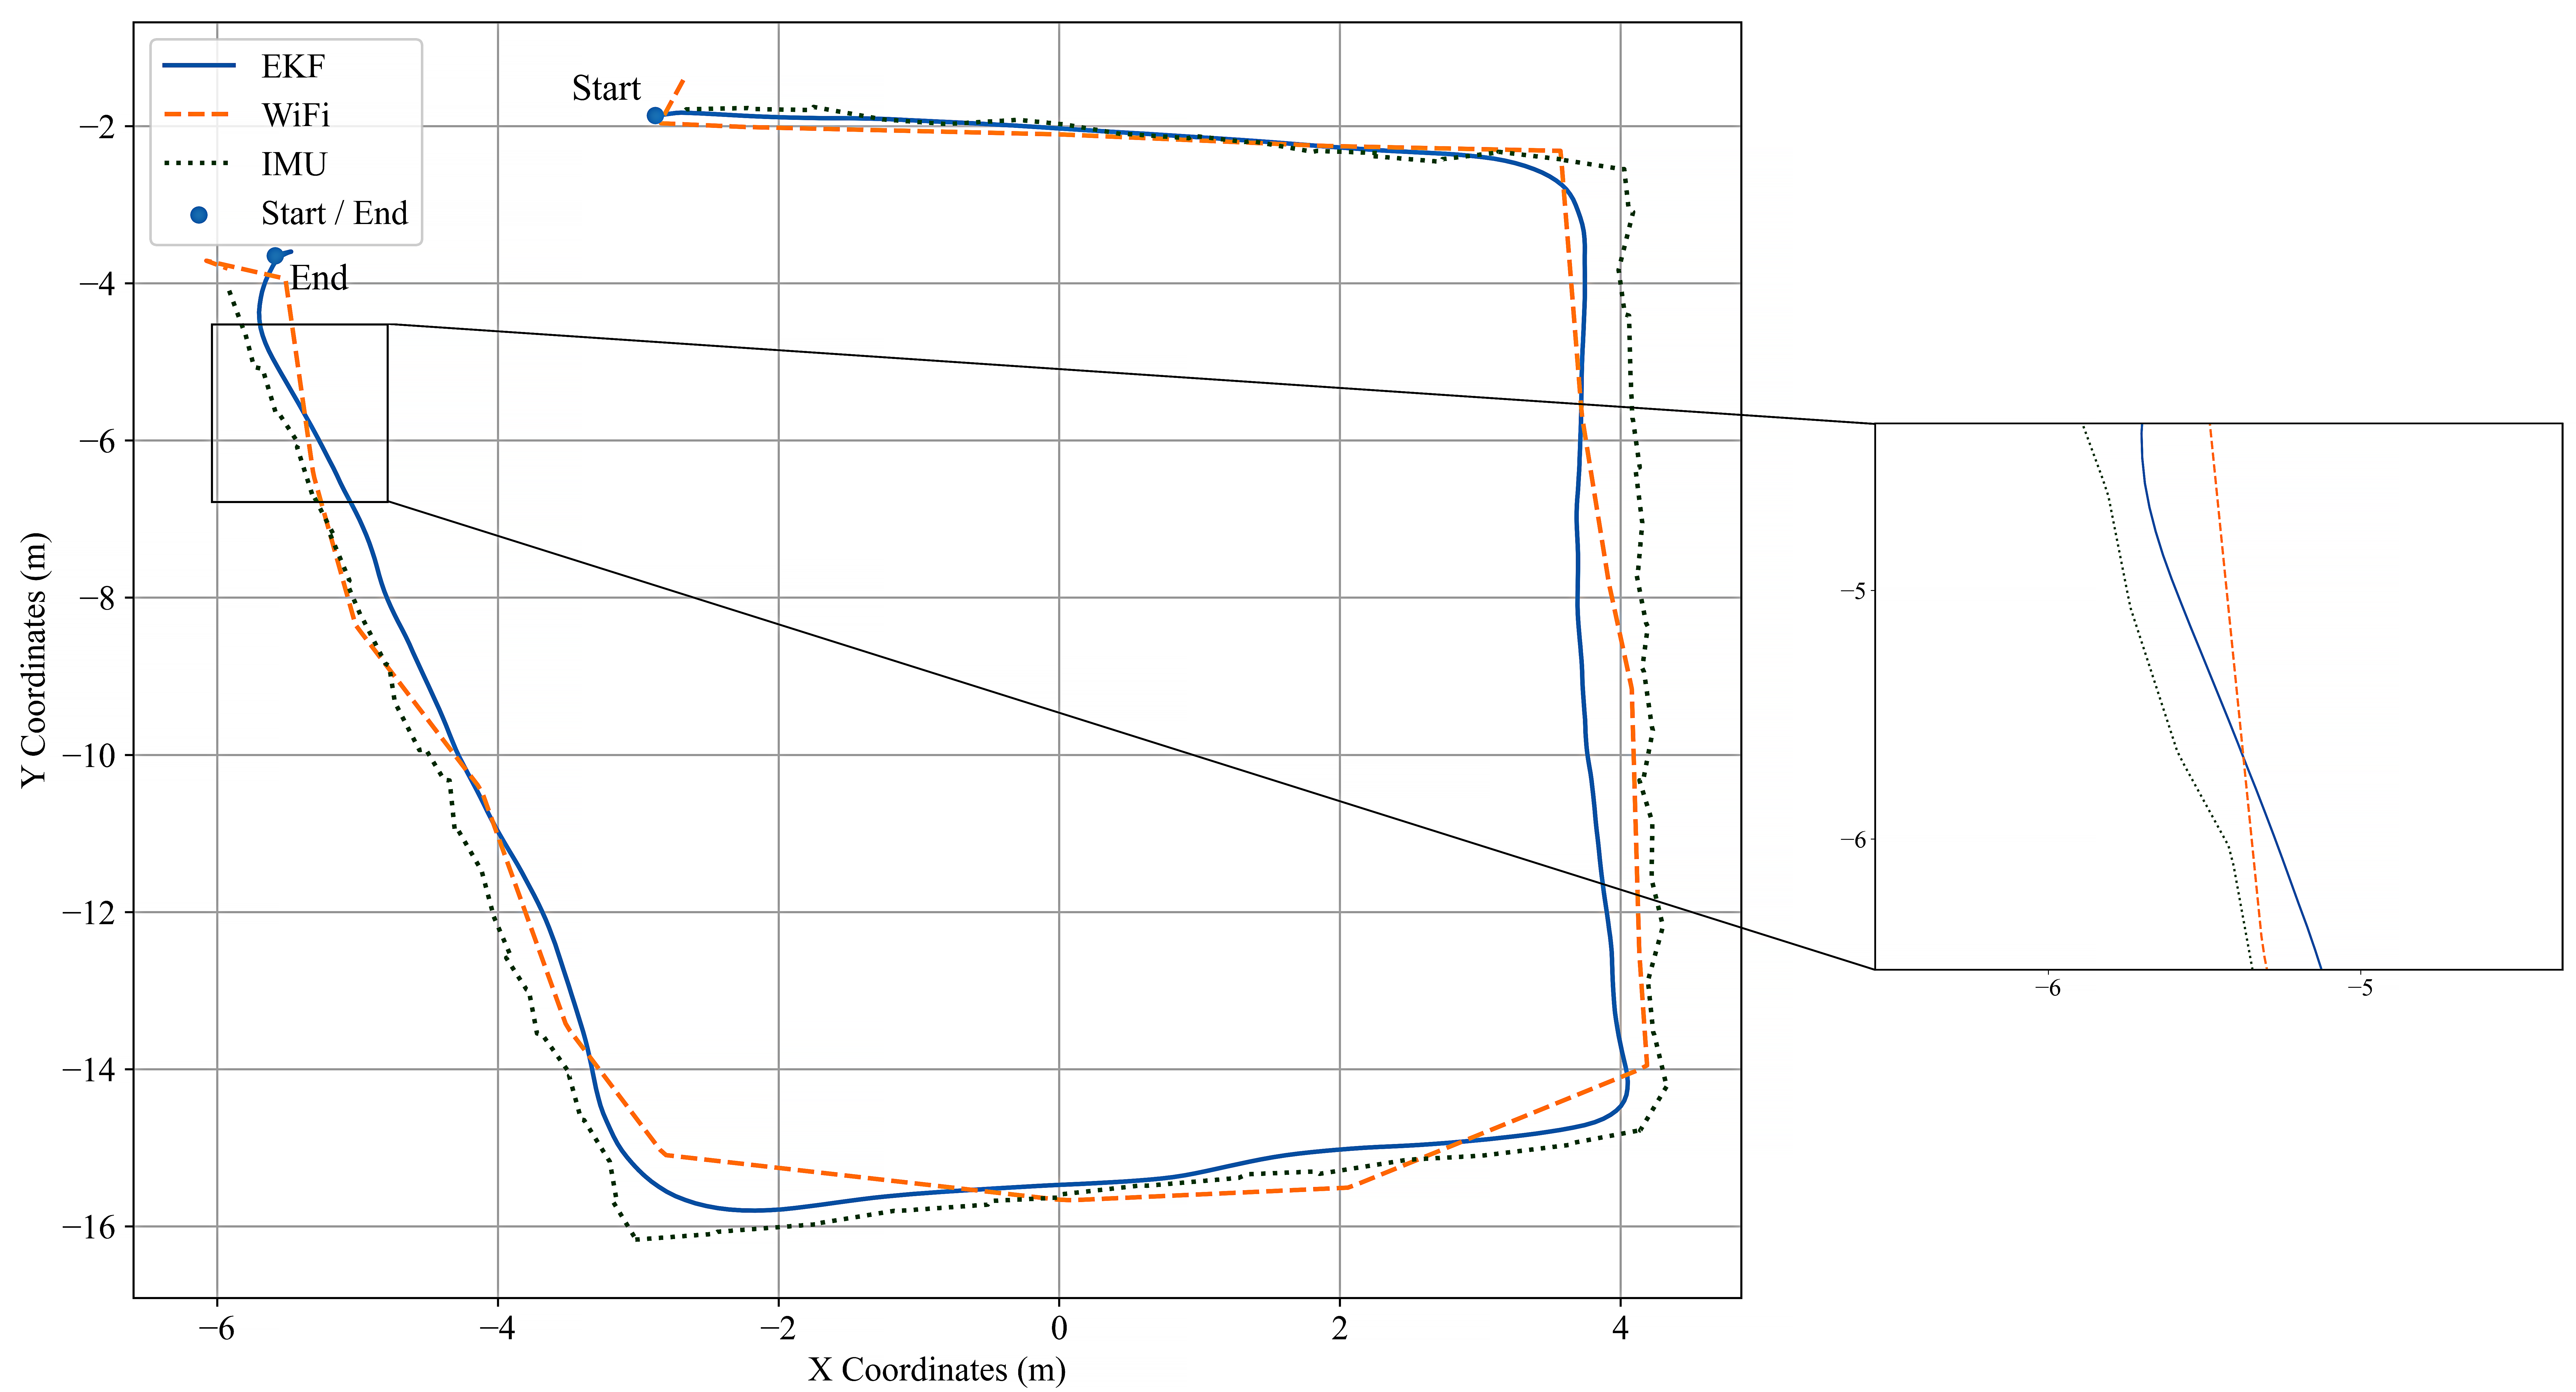
\includegraphics[width=\linewidth]{Amplification
    images/wifi/half_circle_low_diff.png}
  \caption{Amplified image of the error in the comparison of the experimental
    trajectories on the 6th floor.}
  \label{fig:Error amplification diagram 6th}
\end{figure}

After completing the experimental analysis of the sixth and seventh floors, in
order to further verify the generalization ability of the EKF fusion method, we
conducted the same experiment on the eighth floor of the IR building.

As shown in~\autoref{fig:Comparison of experimental trajectories on the 8th
  floor} of the experimental results on the 8th floor of the IR building, Wi-Fi
localization is still affected by the signal environment, exhibiting a certain
degree of drift, and the trajectory error is greater than that on the 6th
floor. In addition, IMU localization is still inaccurate when turning corners
and cannot stably capture the movement of the platform. In contrast, the EKF
method effectively integrates Wi-Fi and IMU data, significantly improving
localization performance and demonstrating greater robustness and stability in
complex environments.
\begin{figure}[H]
  \centering
  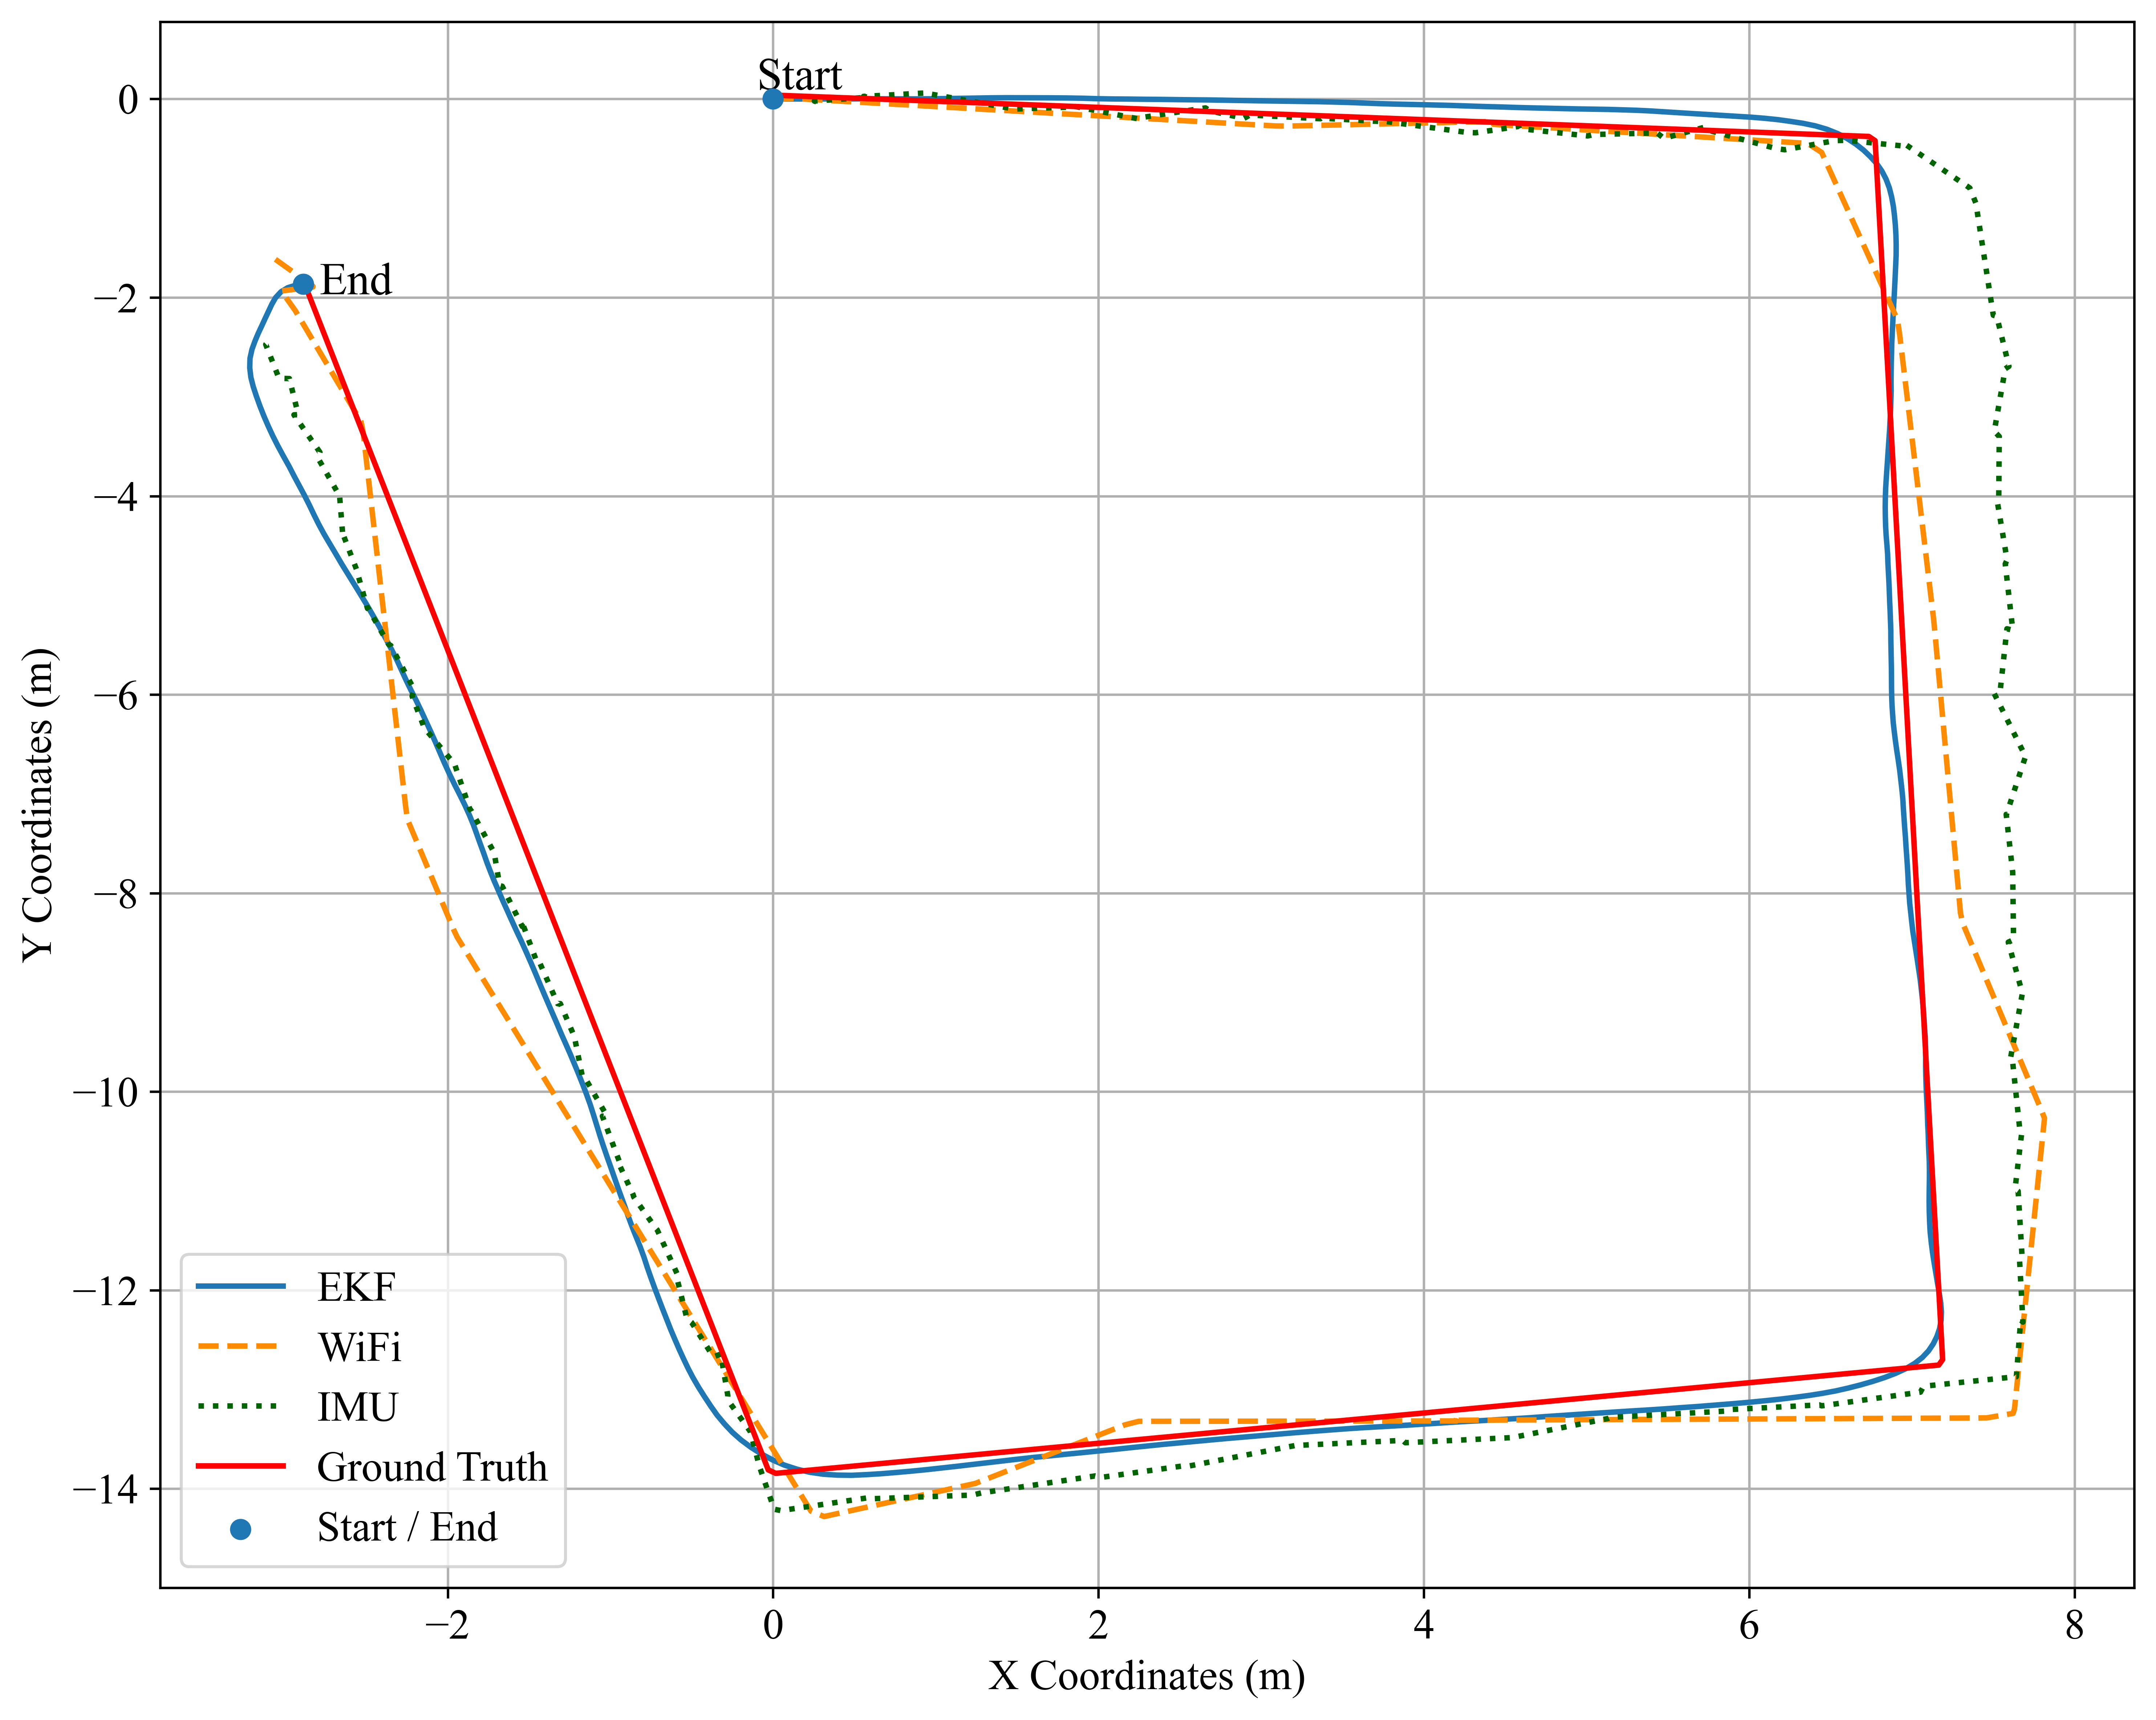
\includegraphics[width=0.7\linewidth]{images/1/1.png}
  \caption{Comparison of experimental trajectories on the 8th floor.}
  \label{fig:Comparison of experimental trajectories on the 8th floor}
\end{figure}

As shown in~\autoref{tab:8thfloor_error}, in the experiment on the 8th floor of
the IR building, the MAE of Wi-Fi localization was 0.5846 and the MSE was
0.8358, indicating that the error of Wi-Fi localization varied greatly, with
good and bad localization effects and considerable instability. This instability
may be closely related to changes in the signal environment (such as signal
obstruction and reflection), resulting in significant differences in the
performance of Wi-Fi localization in different areas.

In contrast, the error variation range of the IMU is relatively small, with an
MAE of 0.8645 and an MSE of 1.7970, indicating that the IMU maintains a
relatively stable error level throughout the experiment. However, due to the
inherent limitations of the sensors, the IMU's accuracy does not improve
significantly in complex dynamic environments (such as when turning), resulting
in larger errors, particularly during rapid movements.
\begin{table}[H]
  \caption{8th floor localization accuracy evaluation (MAE and MSE)}
  \label{tab:8thfloor_error}
  \centering
  \begin{tabular}{lcc}
    \toprule
    \textbf{Localization Method} & \textbf{MAE (m)} & \textbf{MSE (m$^2$)} \\
    \midrule
    Wi-Fi (w.r.t EKF) & 0.5846 & 0.8358 \\
    IMU (w.r.t EKF) & 0.8645 & 1.7970 \\
    EKF (w.r.t Ground Truth) & 0.740 & 1.551 \\
    \bottomrule
  \end{tabular}
\end{table}

Based on the results of local magnification (\autoref{fig:Error amplification
  diagram 8th}), we conclude that the EKF method can effectively combine the
advantages of Wi-Fi and IMU in similar environments on different floors. Through
multiple corrections of sensor data, EKF significantly reduces the accumulation
of errors and provides a smoother and more accurate localization trajectory.
\begin{figure}[H]
  \centering
  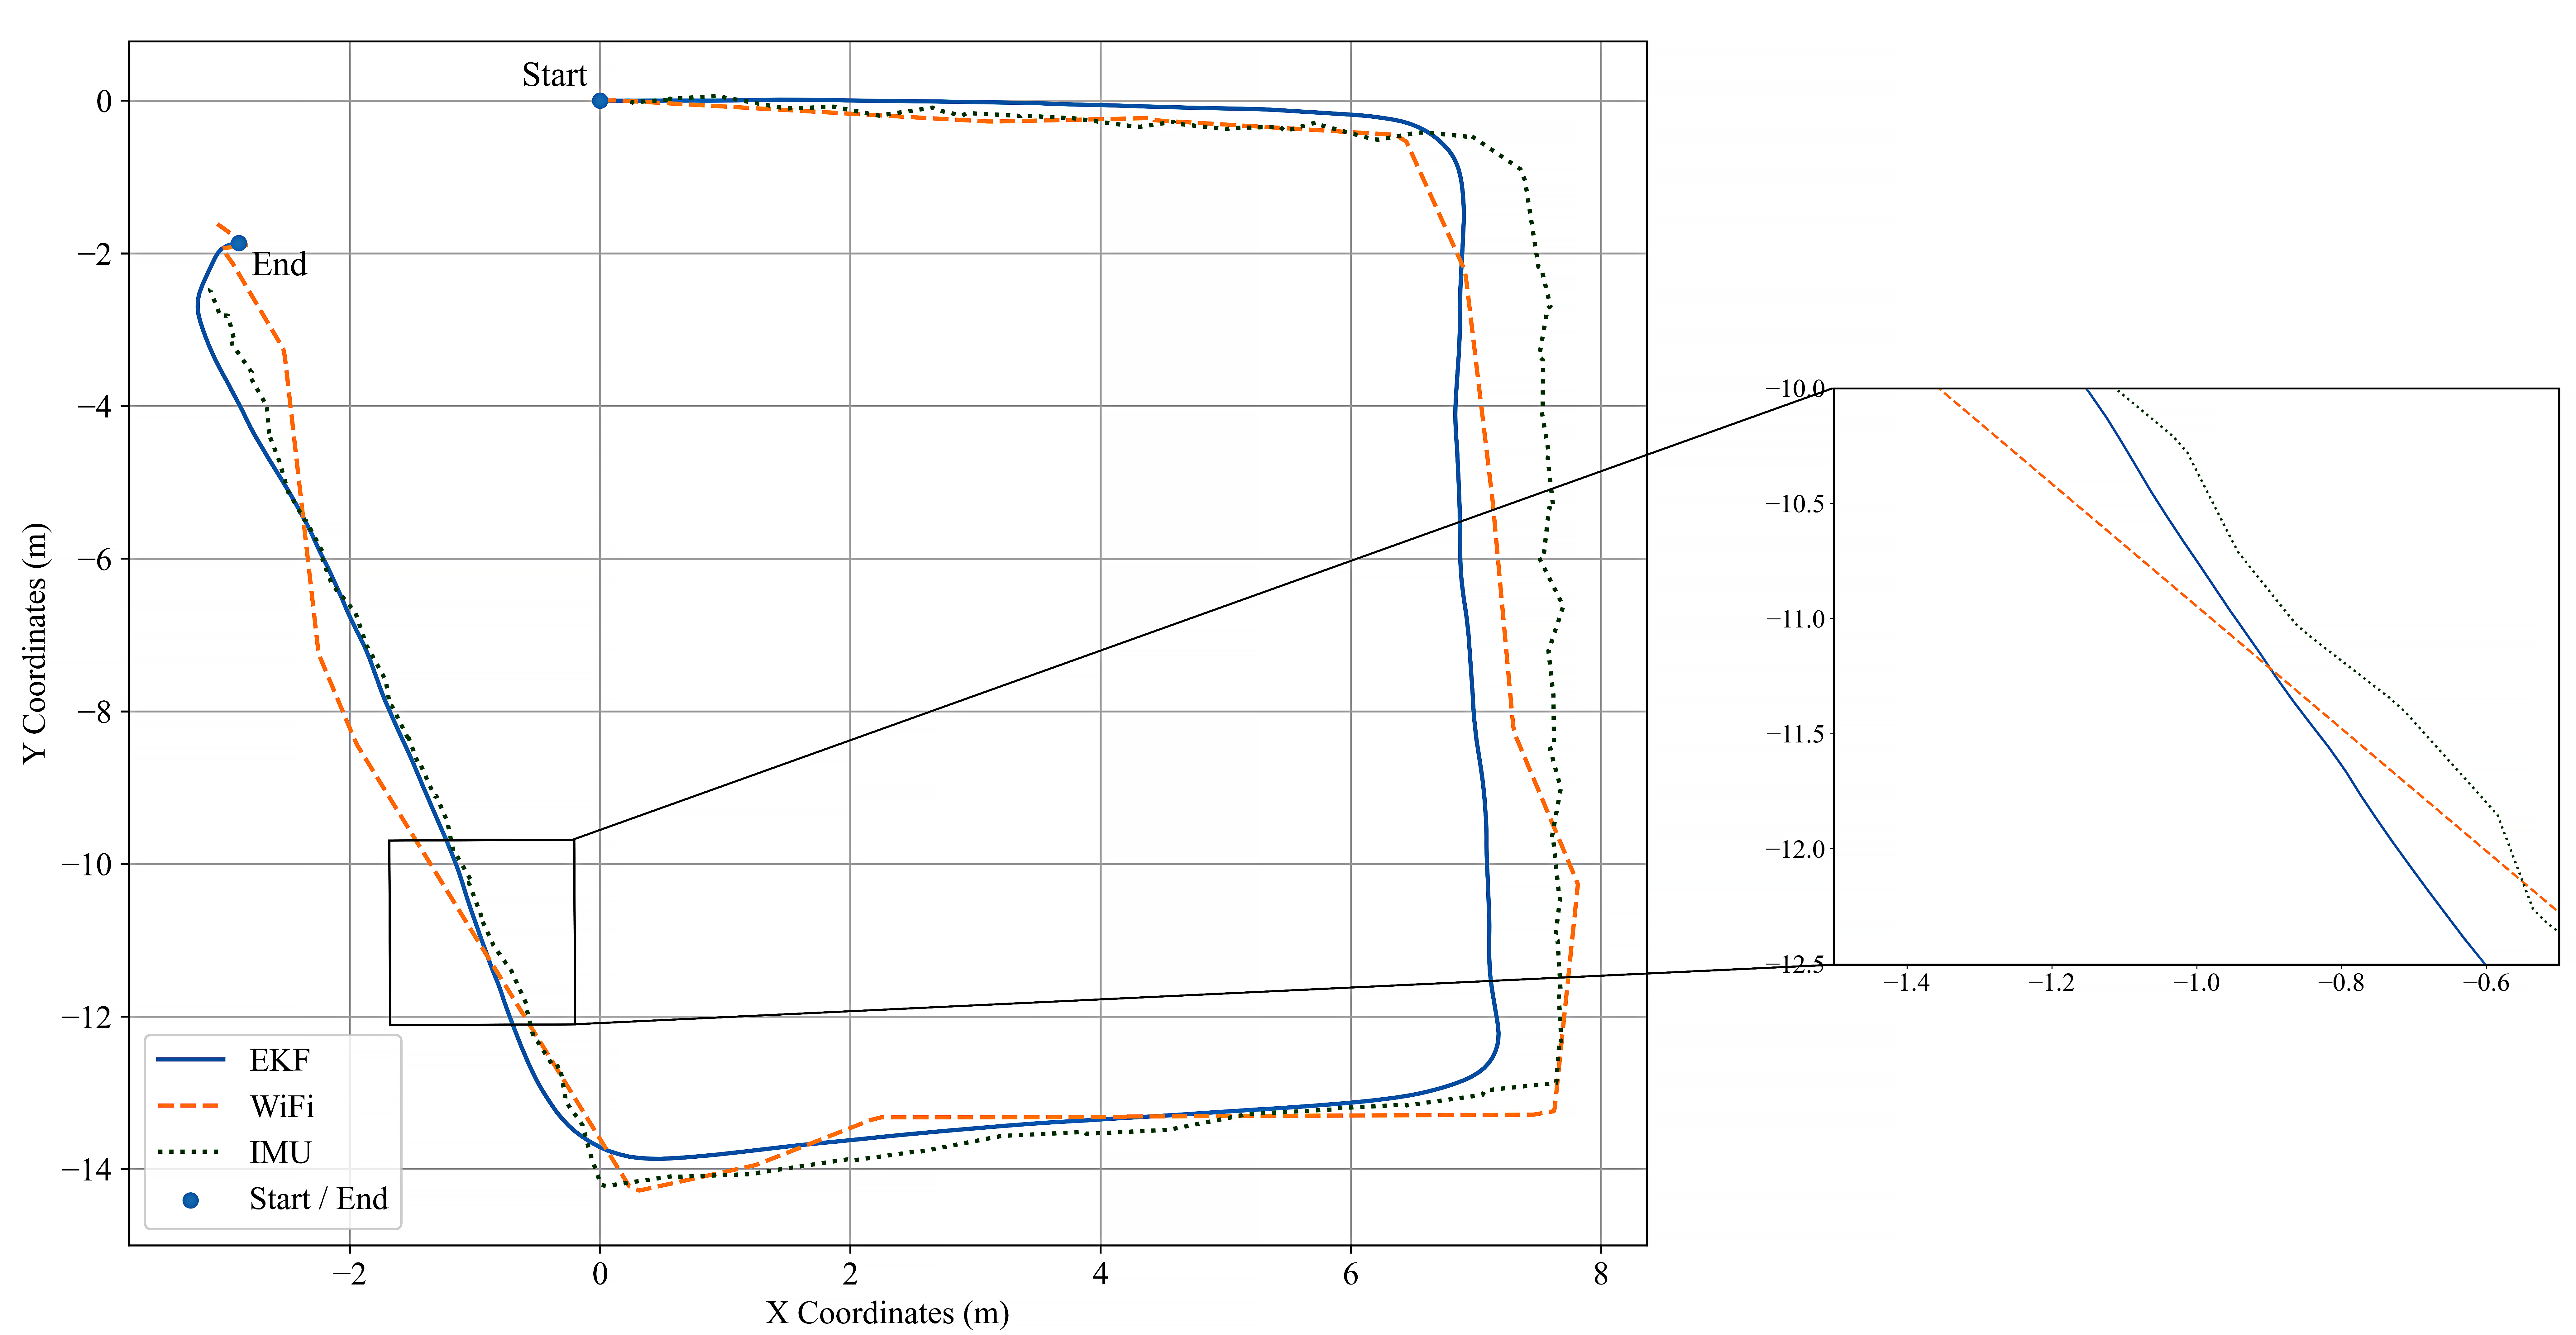
\includegraphics[width=1\linewidth]{Amplification images/wifi/half_circle.png}
  \caption{Amplified image of the error in the comparison of the experimental
    trajectories on the 8th floor.}
  \label{fig:Error amplification diagram 8th}
\end{figure}

\subsection{Full corridor trajectory evaluation on the 7th floor}
In previous experiments, we conducted tests in similar corridor areas on the
6th, 7th, and 8th floors of the IR building. In order to further verify the
stability and robustness of the system in different floor environments, this
experiment was extended to the entire corridor area on the 7th floor. The
specific trajectory is shown in~\autoref{fig:Second phase indoor localization
  experimental path}. The purpose is to evaluate the localization accuracy and
stability of the system over a larger area, especially in longer distances and
more complex environments. By comparing the results with previous experiments
conducted in similar areas, we can validate the system's adaptability across
different spatial scales and further evaluate the robustness and accuracy of
different sensors and fusion methods in real-world applications.
\begin{figure}[H]
  \centering
  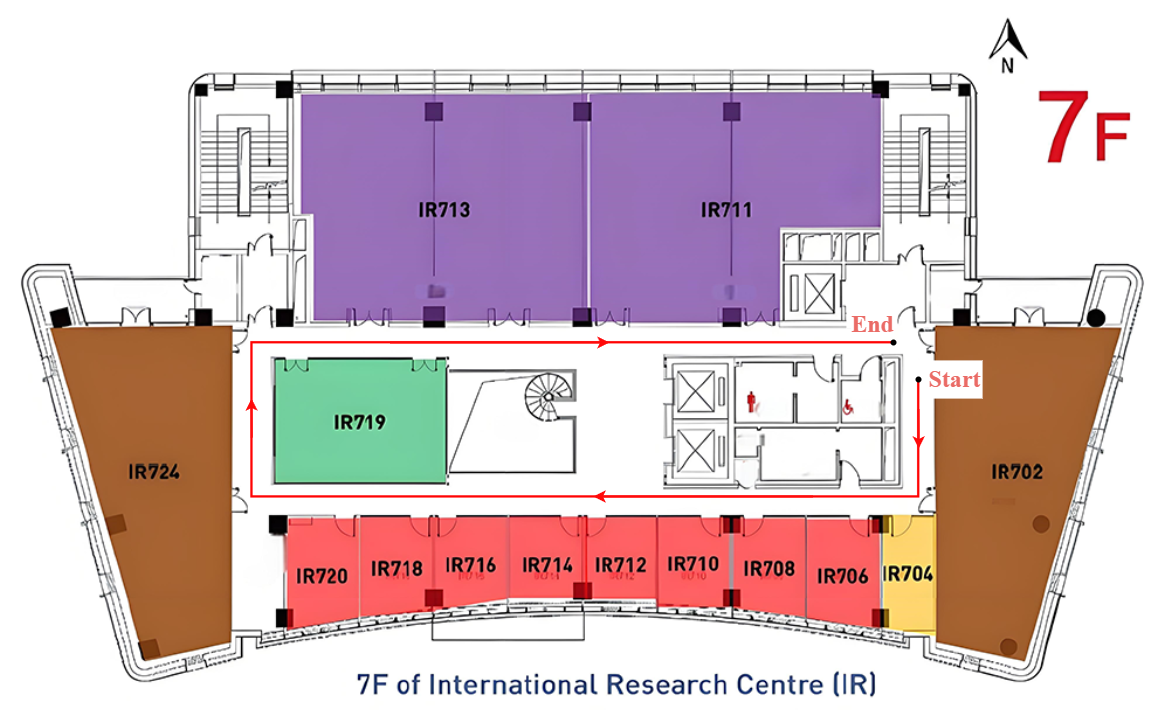
\includegraphics[width=0.9\linewidth]{images/ir_full_circle.png}
  \caption{Second phase indoor localization experimental path.}
  \label{fig:Second phase indoor localization experimental path}
\end{figure}

As can be seen from~\autoref{fig:ir_full_7}, Wi-Fi localization is greatly
affected by the signal environment and exhibits obvious drift. Due to signal
obstruction and the influence of smaller frequencies, the Wi-Fi localization
trajectory is relatively tortuous and cannot provide a smooth
trajectory. Especially on longer paths, the error is more significant, leading
to a decrease in localization accuracy.

In contrast, IMU localization performs relatively smoothly throughout the entire
path. Compared with Wi-Fi, IMU has less error accumulation and can maintain a
relatively stable trajectory on longer paths. However, during rapid movement and
turning, the localization accuracy of the IMU still decreases. Especially when
the direction of movement changes significantly, IMU system errors begin to
accumulate, leading to a further decrease in localization accuracy.

The EKF fusion method provides smoother and more accurate trajectories than
single Wi-Fi and IMU localization methods. In areas with multiple turns and
signal restrictions, EKF can effectively reduce errors and optimize localization
results. By integrating information from different sensors, it compensates for
their respective shortcomings and significantly improves localization accuracy.
\begin{figure}[H]
  \centering
  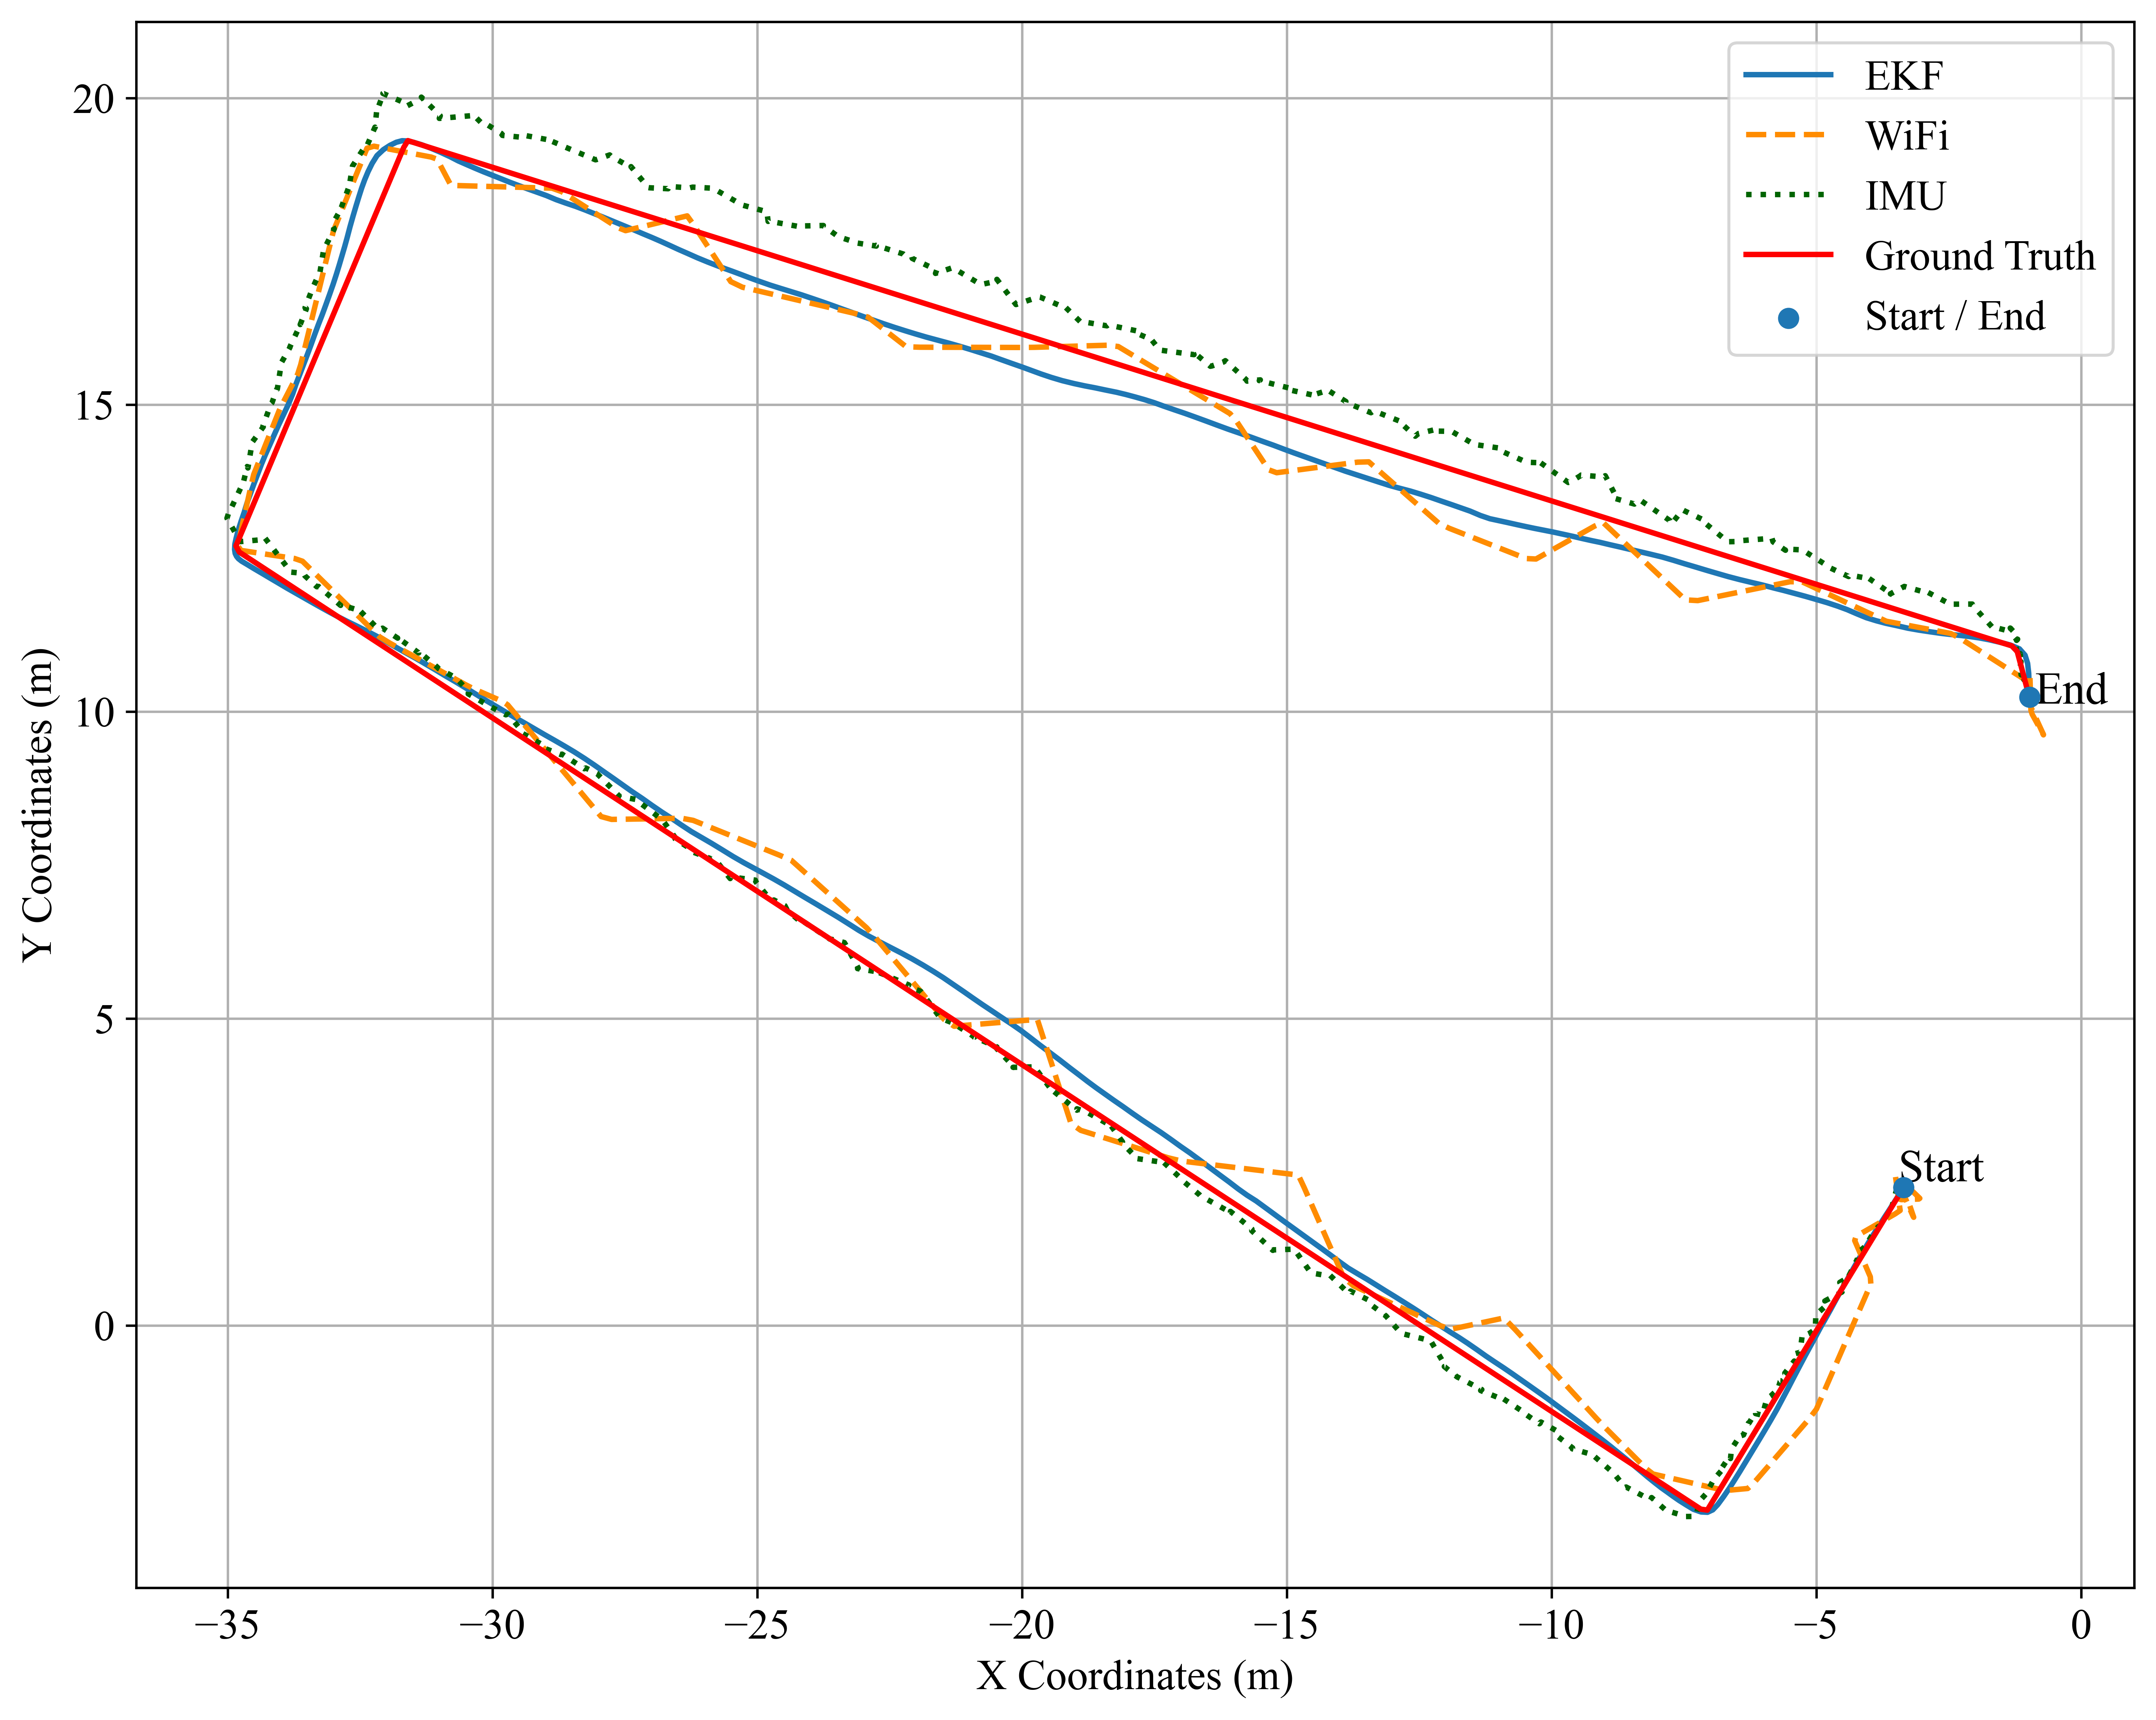
\includegraphics[width=0.8\linewidth]{images/1/3.png}
  \caption{Comparison of experimental results trajectories in the entire
    corridor on the 7th floor of the IR building.}
  \label{fig:ir_full_7}
\end{figure}

According to~\autoref{tab:7th_floor_accuracy}, the MAE of Wi-Fi localization is
0.2251 and the MSE is 0.0778, indicating that the overall error is
small. However, Wi-Fi localization showed large fluctuations in the experiment,
which was due to factors such as signal obstruction and reflection. Wi-Fi
localization is based on RSSI signals, which are greatly affected by obstacles
and multipath effects, resulting in uneven or tortuous trajectories in some
areas. Nevertheless, Wi-Fi localization can still provide relatively accurate
location estimates at some times, thereby maintaining low MAE and MSE values.

The MAE of the IMU is 0.6655, and the MSE is 0.8059, showing a reduction in
error compared to previous experiments with shorter paths. This indicates that
although errors still exist in longer paths, the overall error has improved
compared to previous tests. The IMU can provide relatively stable platform
position information, but error accumulation remains one of its main issues in
dynamic environments. Through experiments on longer paths, the performance of
the IMU in more complex environments can be verified, and it is further
demonstrated that it can maintain relatively small errors under relatively
stable conditions.
\begin{table}[H]
  \centering
  \caption{Accuracy assessment of localization of entire path on 7th floor}
  \label{tab:localization_error}
  \begin{tabular}{lcc}
    \toprule
    \textbf{Localization Method} & \textbf{MAE (m)} & \textbf{MSE (m\textsuperscript{2})} \\
    \midrule
    Wi-Fi (w.r.t EKF) & 0.2251 & 0.0778 \\
    IMU (w.r.t EKF)   & 0.6655 & 0.8059 \\
    EKF (w.r.t Ground Truth)    & 0.5290 & 0.6010 \\
    \bottomrule
  \end{tabular}
\end{table}

As shown in the enlarged view in~\autoref{fig:error_full_7}, it can be clearly
seen that the Wi-Fi localization trajectory has large fluctuations. At the same
time, the IMU localization trajectory is slightly smoother than the Wi-Fi, but
there are still errors. The IMU errors have a certain accumulation effect,
causing the trajectory to deviate from the actual path. In comparison, it can be
seen that the trajectory provided by EKF is smoother and more accurate than
Wi-Fi and IMU.
\begin{figure}[H]
  \centering
  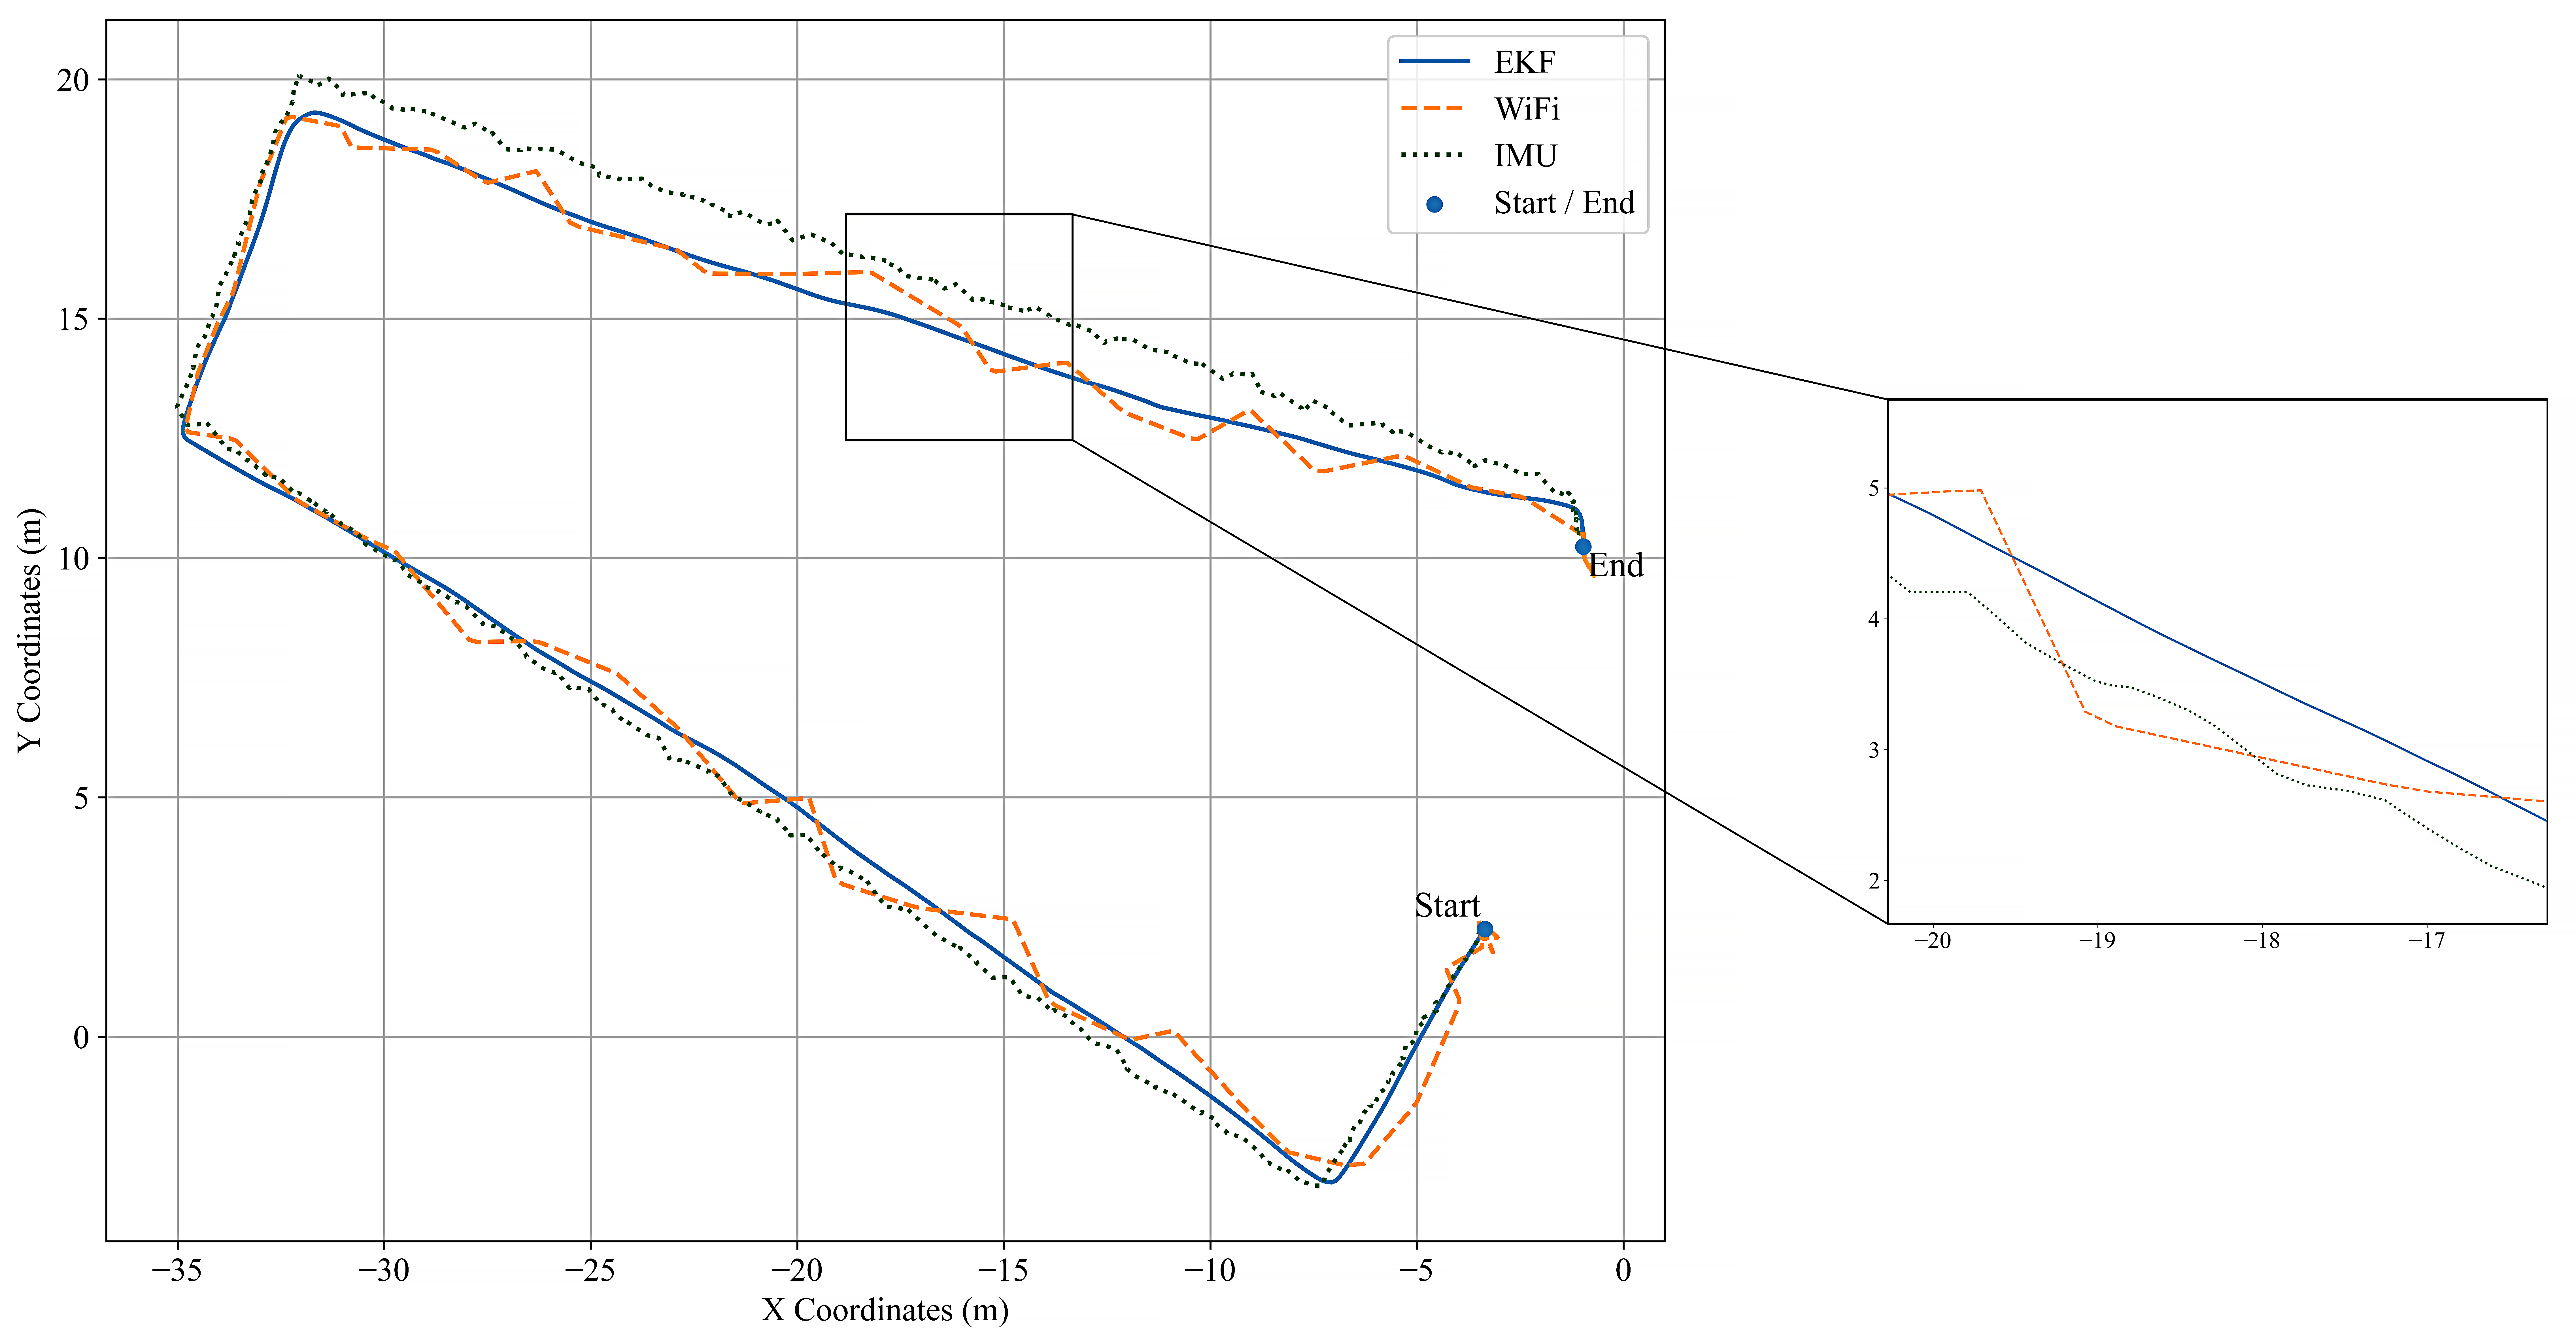
\includegraphics[width=1\linewidth]{Amplification images/wifi/full_circle.png}
  \caption{Enlarged image of the comparison error in the entire corridor on the
    7th floor of the IR building.}
  \label{fig:error_full_7}
\end{figure}

\subsection{Evaluation under reversed start and end points}
In the experiment above, we demonstrated the complete path experiment results on
the 7th floor. In order to further verify the performance of the system at
different start and end location, the path on the 7th floor was adjusted in this
experiment, changing the start and end location, as shown in~\autoref{fig:Indoor
  localization experiment path after changing location}. Through this
adjustment, we aimed to examine the localization consistency and accuracy of the
system when the path direction changes, thereby further verifying its
adaptability and robustness in practical applications.
\begin{figure}[H]
  \centering
  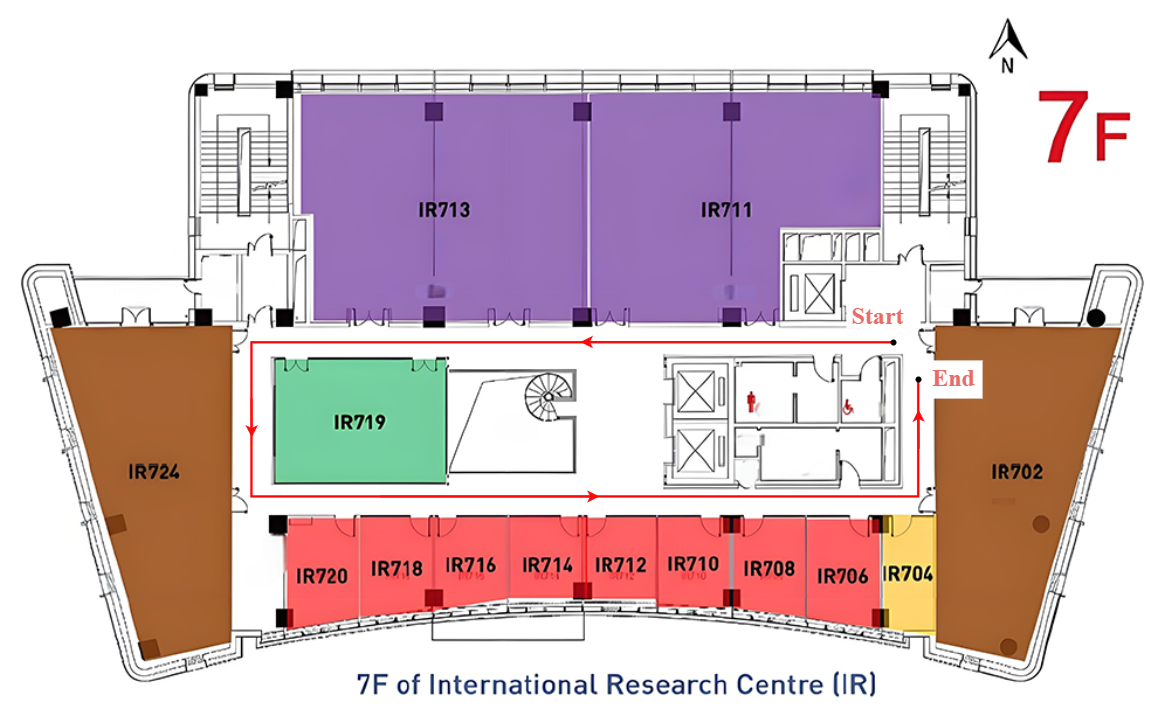
\includegraphics[width=0.9\linewidth]{images/ir_full_circle_inverse.png}
  \caption{Indoor localization experiment path after changing location.}
  \label{fig:Indoor localization experiment path after changing location}
\end{figure}

\autoref{fig:Complete path comparison of IR building 7th floor experiment
  trajectory (start and end locations swapped)} shows the comparison results of
the trajectories obtained by swapping the starting and ending positions along
the complete corridor path on the 7th floor of the IR building. The experimental
path remains consistent with the previous complete corridor experiment, with
only the direction of movement altered. This is aimed at evaluating the system's
stability and consistency under changes in path direction.

As can be seen from~\autoref{fig:Complete path comparison of IR building 7th
  floor experiment trajectory (start and end locations swapped)}, the Wi-Fi
trajectory still exhibits significant fluctuations at the long path positions
near the endpoint, indicating that it is susceptible to interference from signal
obstruction or multipath effects and has poor stability. The IMU trajectory is
generally smooth, but error accumulation still occurs during long path travel,
causing the trajectory to deviate from the actual path gradually. In contrast,
the EKF fusion method maintains stable, continuous, and accurate path estimation
even after changing the path direction, fully demonstrating its robustness and
adaptability to changes in travel direction and environmental conditions under
multi-source information fusion.

\begin{figure}[H]
  \centering
  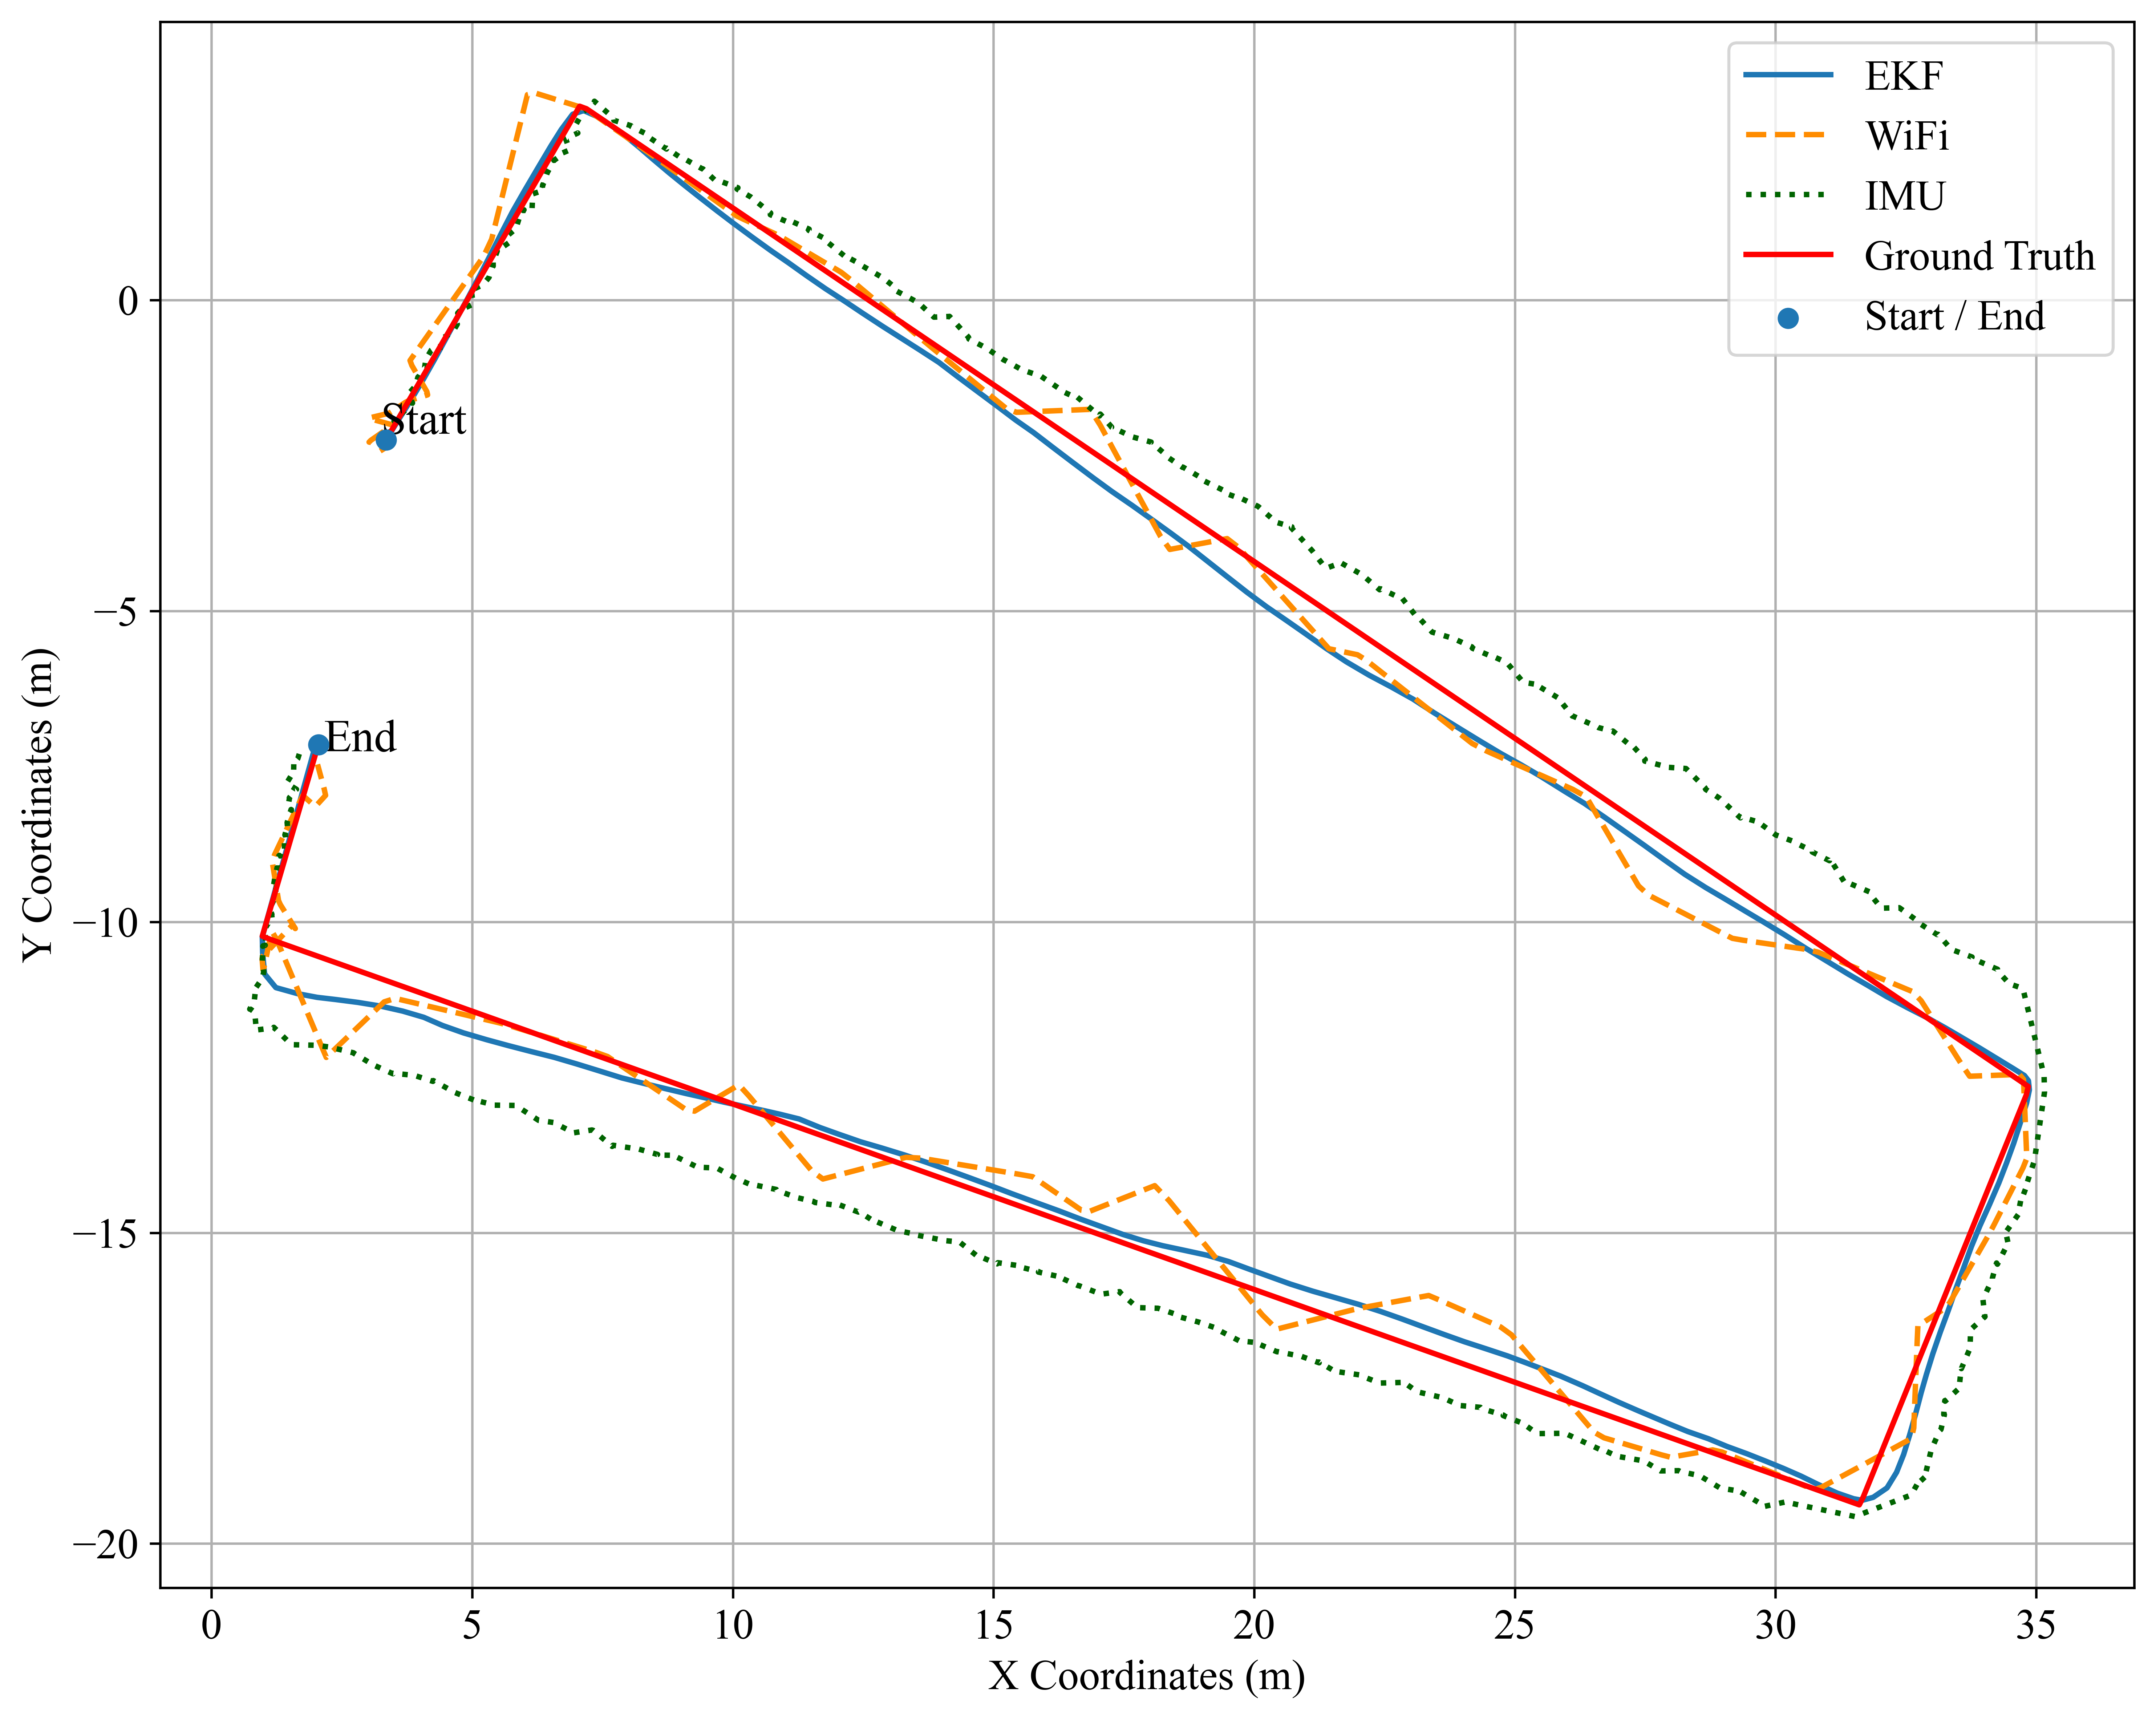
\includegraphics[width=0.8\linewidth]{images/1/0.png}
  \caption{Complete path comparison of IR building 7th floor experiment
    trajectory (start and end locations swapped).}
  \label{fig:Complete path comparison of IR building 7th floor experiment
    trajectory (start and end locations swapped)}
\end{figure}

In the experiment where the starting and ending positions of the complete
corridor path were swapped, the error metrics of Wi-Fi and IMU exhibited trends
consistent with previous experiments but also showed some differences. As shown
in~\autoref{tab:7th_inverse_accuracy}, the Wi-Fi MAE was 0.2493 and the MSE was
0.1038, slightly higher than the MAE (0.2251) and MSE (0.0778) obtained in the
previous experiment with the same path but in the opposite direction. This
indicates that Wi-Fi became slightly more sensitive to changes in the local
signal environment after the path direction was changed, with more significant
fluctuations observed near the start and end regions.

The MAE and MSE of IMU are 0.8494 and 1.1384, respectively. Although they still
exhibit a trend of error accumulation over time, they have increased compared to
the previous experiment's MAE (0.6655) and MSE (0.8059), indicating that the
change in travel direction may have exacerbated the cumulative effect of
attitude estimation errors at different turning nodes.

Overall, although Wi-Fi and IMU exhibited some degree of error fluctuation under
changes in the direction of travel, the EKF fusion method maintained good
stability and accuracy in this experiment.
\begin{table}[H]
  \centering
  \caption{7th floor inverse-path localization accuracy evaluation (MAE and
    MSE)}
  \label{tab:7th_inverse_accuracy}
  \begin{tabular}{lcc}
    \toprule
    \textbf{Localization Method} & \textbf{MAE (m)} & \textbf{MSE (m\textsuperscript{2})} \\
    \midrule
    Wi-Fi (w.r.t EKF) & 0.2493 & 0.1038 \\
    IMU (w.r.t EKF) & 0.8494 & 1.1384 \\
    EKF (w.r.t Ground Truth) & 0.8830 & 1.9050 \\
    \bottomrule
  \end{tabular}
\end{table}

\autoref{fig:error_7_inverse} shows a magnified view of the complete path
experiment after swapping the start and end positions, focusing on the corner
area where Wi-Fi errors are relatively large. As can be seen from the figure,
the Wi-Fi trajectory shows a significant deviation in this section, with a huge
trajectory jump at the corner. The IMU trajectory, on the other hand, exhibits a
relatively smooth trend overall, but also shows signs of error accumulation in
this area, primarily manifested as a continuous deviation in the trajectory. In
contrast, the EKF fusion trajectory maintains good smoothness and spatial
consistency in this area, accurately following the actual movement path.
\begin{figure}[H]
  \centering
  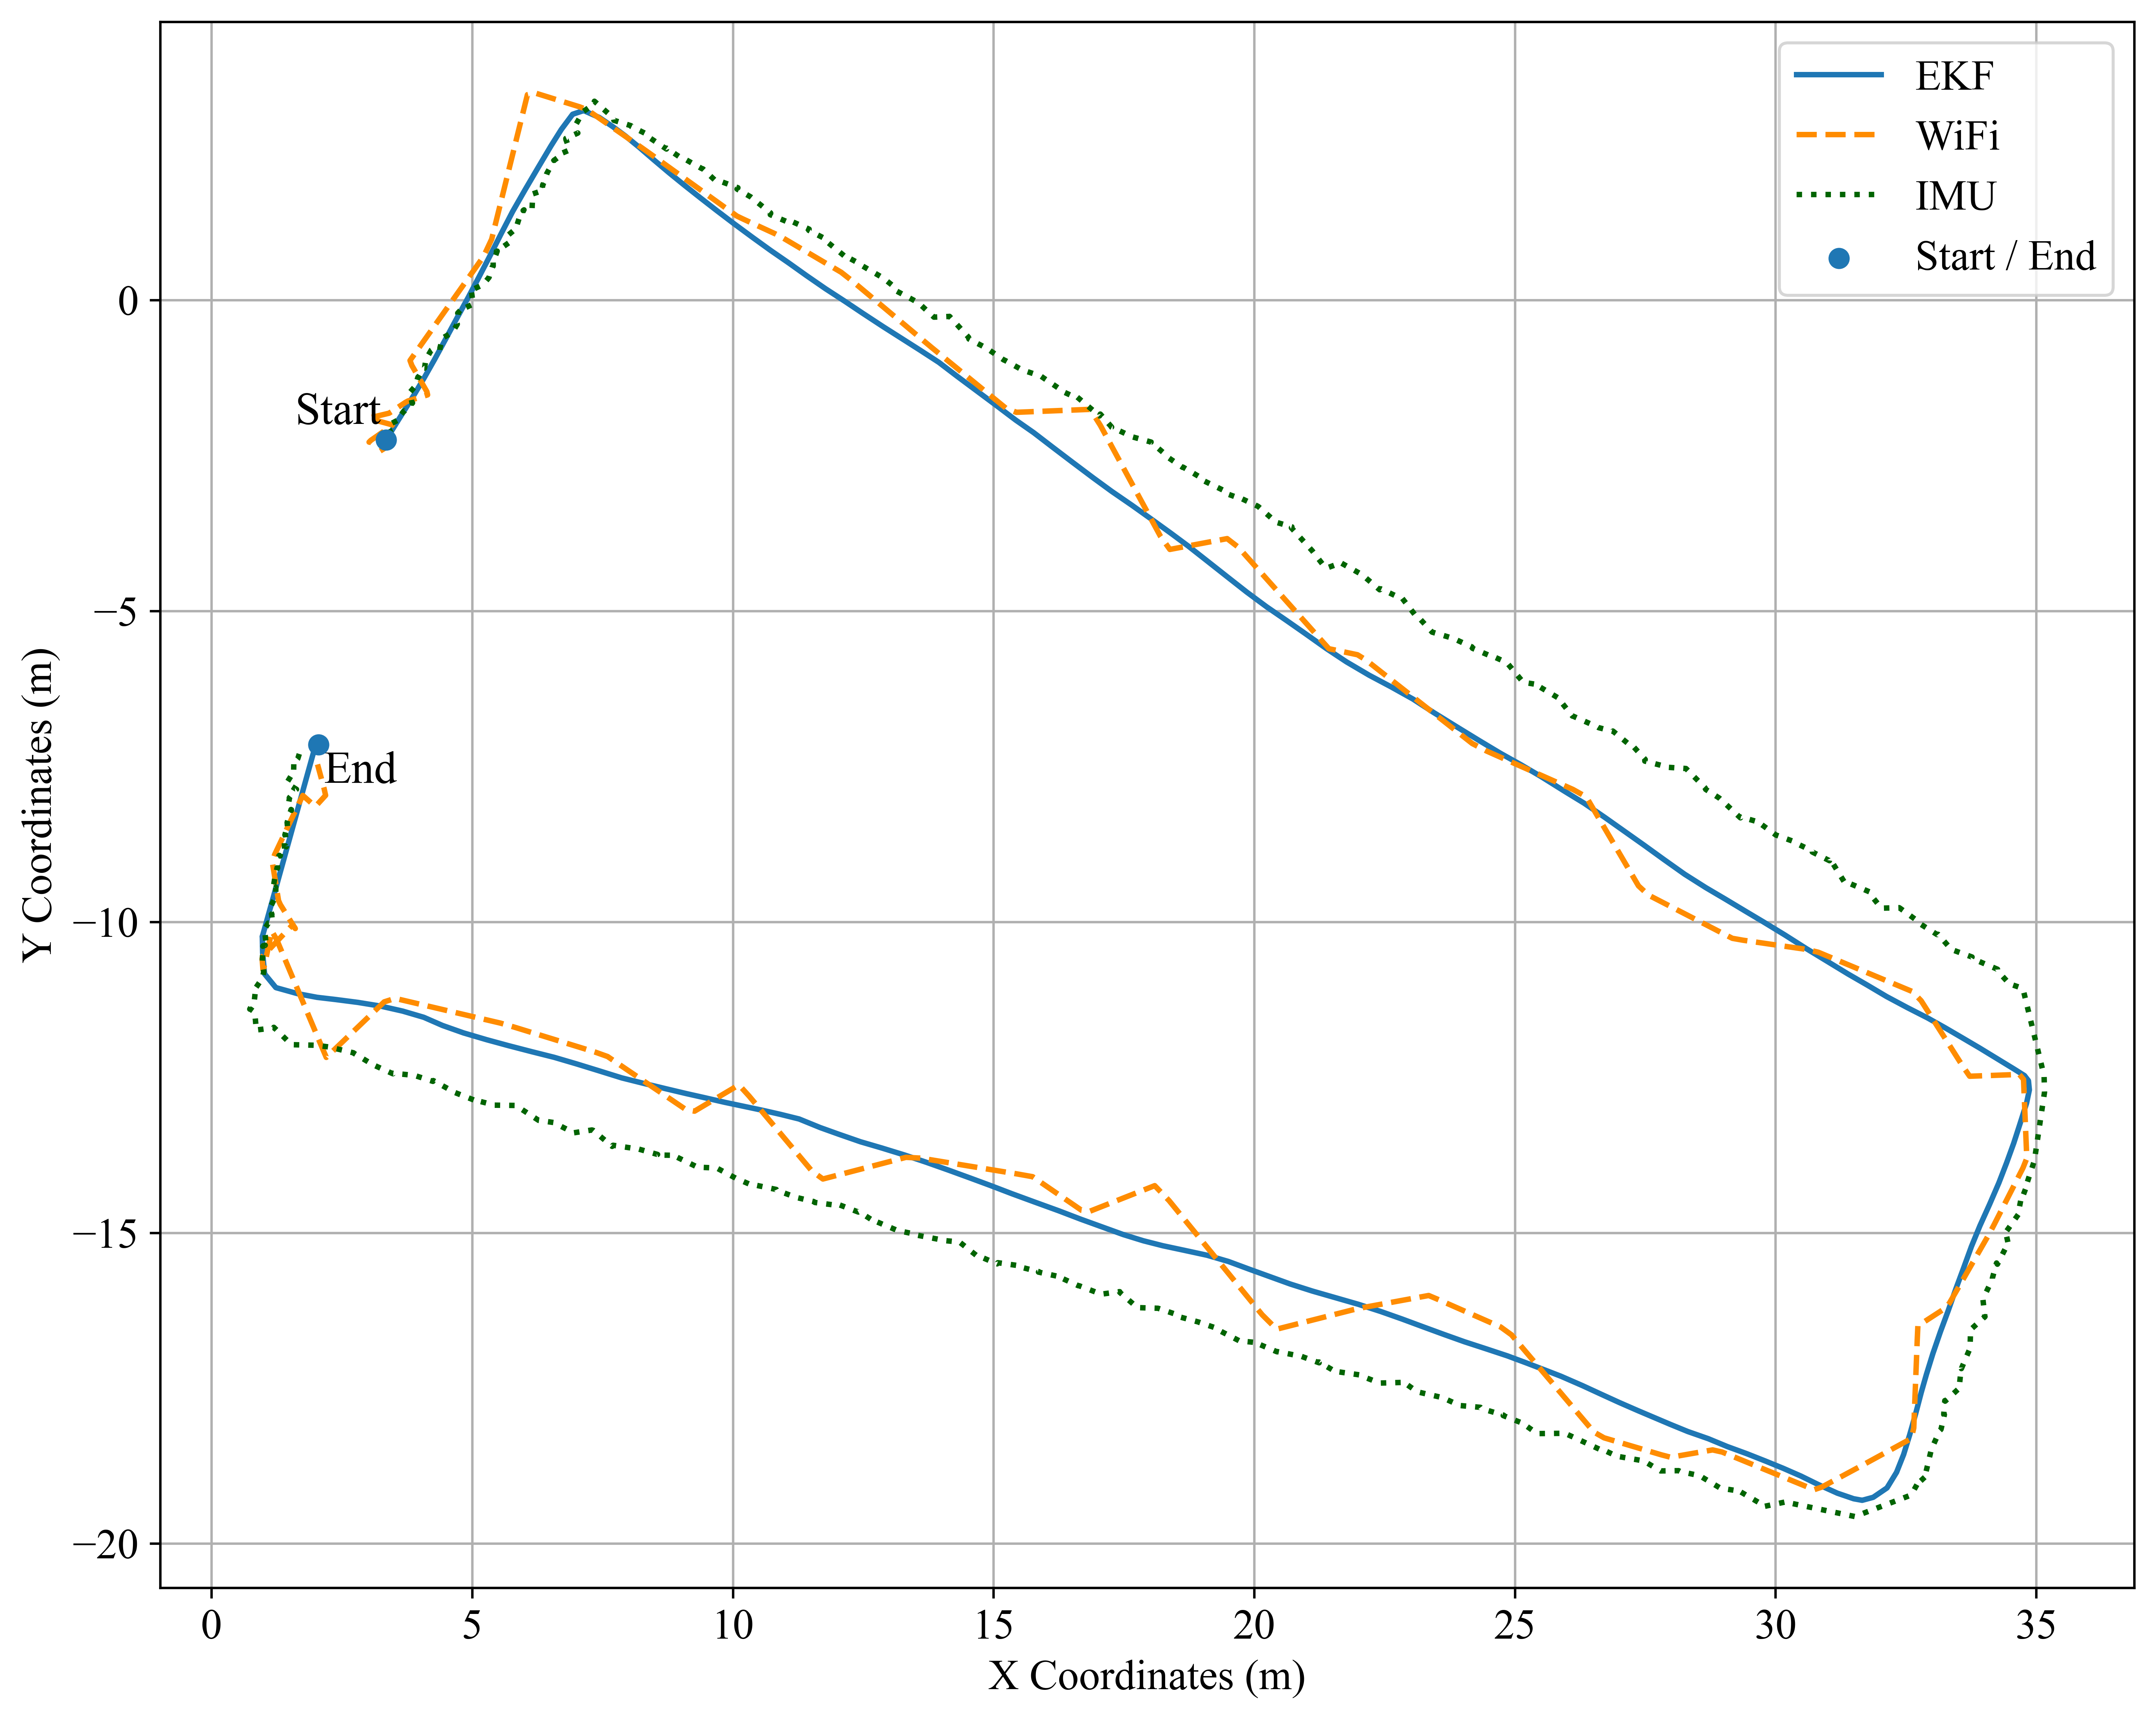
\includegraphics[width=\linewidth]{Amplification
    images/wifi/full_circle_inverse.png}
  \caption{Enlarged image of the comparison error in the entire corridor on the
    7th floor of the IR building (start and end locations swapped).}
  \label{fig:error_7_inverse}
\end{figure}

  
\newpage  
\section{Discussion and Limitations}
Despite the demonstrated effectiveness of the proposed fusion localization
framework, several limitations remain that warrant further investigation:

\begin{itemize}
\item \textbf{Instability and limited generalization of Wi-Fi fingerprinting:}
  Although the Wi-Fi fingerprinting model performs robustly in most areas, the
  RSSI is highly susceptible to multipath propagation, obstruction, and
  environmental variations. These factors introduce considerable measurement
  uncertainty and hinder the model’s generalization across different
  locations. In particular, localization accuracy degrades significantly in
  areas with sparse reference points or strong signal occlusion. Additionally,
  the low update rate of Wi-Fi signals—typically on the order of
  seconds—limits the system’s responsiveness to rapid platform dynamics,
  resulting in delayed positional updates during fast movement or turning.

\item \textbf{Drift and error accumulation in IMU measurements:} The inertial
  measurement unit (IMU) provides high-frequency motion data with strong
  short-term responsiveness. However, its accelerometers and gyroscopes are
  vulnerable to noise and bias drift, leading to cumulative errors over
  time. Without timely correction from external observations (e.g., SLAM), the
  IMU's estimations diverge from the actual trajectory, which negatively
  affects the overall accuracy and robustness of the system.

\item \textbf{Sensitivity of SLAM to dynamic and occluded environments:}
  Although SLAM contributes mid-frequency structural constraints, its
  loop-closure performance can be compromised in dynamic scenes or environments
  with significant occlusions. This weakens the consistency and accuracy of the
  state updates performed by the EKF.

\item \textbf{Limited diversity in experimental settings:} The experiments were
  conducted in campus buildings characterized by long corridors and regular
  spatial layouts. While representative, the system’s adaptability to open
  spaces, highly dynamic settings, or crowded public environments remains
  unverified. Further studies should extend the evaluation to more diverse and
  challenging scenarios.

\item \textbf{Lack of adaptive parameter tuning in the EKF model:} The
  performance of the system relies heavily on the manual configuration of EKF
  parameters, particularly the process and measurement noise covariance
  matrices. These parameters significantly influence the filter’s convergence
  and localization accuracy. Future work should consider the integration of
  adaptive tuning strategies, such as Bayesian optimization or reinforcement
  learning, to enhance the model’s adaptability and reduce dependency on manual
  calibration.
\end{itemize}


\newpage
\section{Conclusion and Future work}
\subsection{Conclusion}
In summary, this study proposes and evaluates a robust multi-sensor indoor
localization system. The main conclusions are as follows:

\begin{itemize}
\item \textbf{A novel fusion framework} was developed by integrating Wi-Fi
  fingerprinting, LiDAR-based SLAM, and EKF, effectively addressing the
  limitations of single-modality localization in complex indoor environments.
  
\item \textbf{The DNN-based Wi-Fi localization approach} successfully captures
  the nonlinear relationship between RSSI and spatial position, resulting in
  improved localization accuracy over traditional methods.
  
\item \textbf{The Gmapping-based SLAM algorithm} enables efficient real-time
  environment mapping and localization, enhancing the system's adaptability and
  robustness in dynamic and cluttered environments.
  
\item \textbf{The EKF-based data fusion module} significantly improves
  localization stability by suppressing Wi-Fi signal fluctuations and mitigating
  IMU drift, leading to more accurate and smooth trajectory estimation.
  
\item \textbf{Extensive real-world experiments} were conducted across multiple
  floors and diverse routes, validating the system’s performance,
  generalizability, and feasibility for practical deployment in real indoor
  environments.
\end{itemize}

\subsection{Future Work}
Given the limitations of this study, future work can be further expanded and
optimized in the following directions:

\begin{itemize}
\item \textbf{Enhancing system robustness:} More heterogeneous sensors, such as
  UWB, visual information, or BLE, can be introduced to enhance the system's
  adaptability to complex indoor environments, multi-path interference, and
  signal occlusion, thereby improving its robustness in response to
  environmental fluctuations.
    
\item \textbf{3D LiDAR and advanced SLAM integration:} Future research may
  consider upgrading the 2D LiDAR to a 3D LiDAR sensor and combining it with
  real-time point cloud processing technologies. More advanced SLAM algorithms,
  such as FAST-LIO2, can be introduced to construct high-precision,
  high-robustness 3D maps, improving the system's perception and localization
  capabilities in multi-floor and multi-structure environments.
    
\item \textbf{Incorporating deep learning models:} Deep learning techniques,
  particularly temporal modelling structures such as RNNs, GRUs, or
  Transformers, can be applied to estimate localization trajectories in an
  end-to-end manner. This would enhance the system's ability to model non-linear
  and dynamic state transitions. Additionally, exploring self-supervised or
  weakly supervised learning frameworks could reduce reliance on labelled
  trajectory datasets.
    
\item \textbf{Online learning and incremental mapping:} Incorporating online
  learning mechanisms and incremental map updating strategies could further
  improve the system's adaptability during long-term deployment, enabling
  continuous optimization of localization accuracy and environmental modelling.
    
\item \textbf{Embedded deployment and system validation:} The current system
  could be ported to an embedded platform (e.g., NVIDIA Jetson Orin Nano) to
  perform real-time testing. This would allow for a comprehensive evaluation of
  the system's power consumption, resource scheduling efficiency, and latency
  performance, laying a foundation for practical deployment in mobile robotics
  and indoor navigation applications.
\end{itemize}


\bibliographystyle{IEEEtran}
\bibliography{IEEEabrv,References}


\newpage

\appendix 
\renewcommand{\thesection}{Appendix~\Alph{section}}

\section{Localization Experiment Path}
\begin{figure}[H]
  \centering
  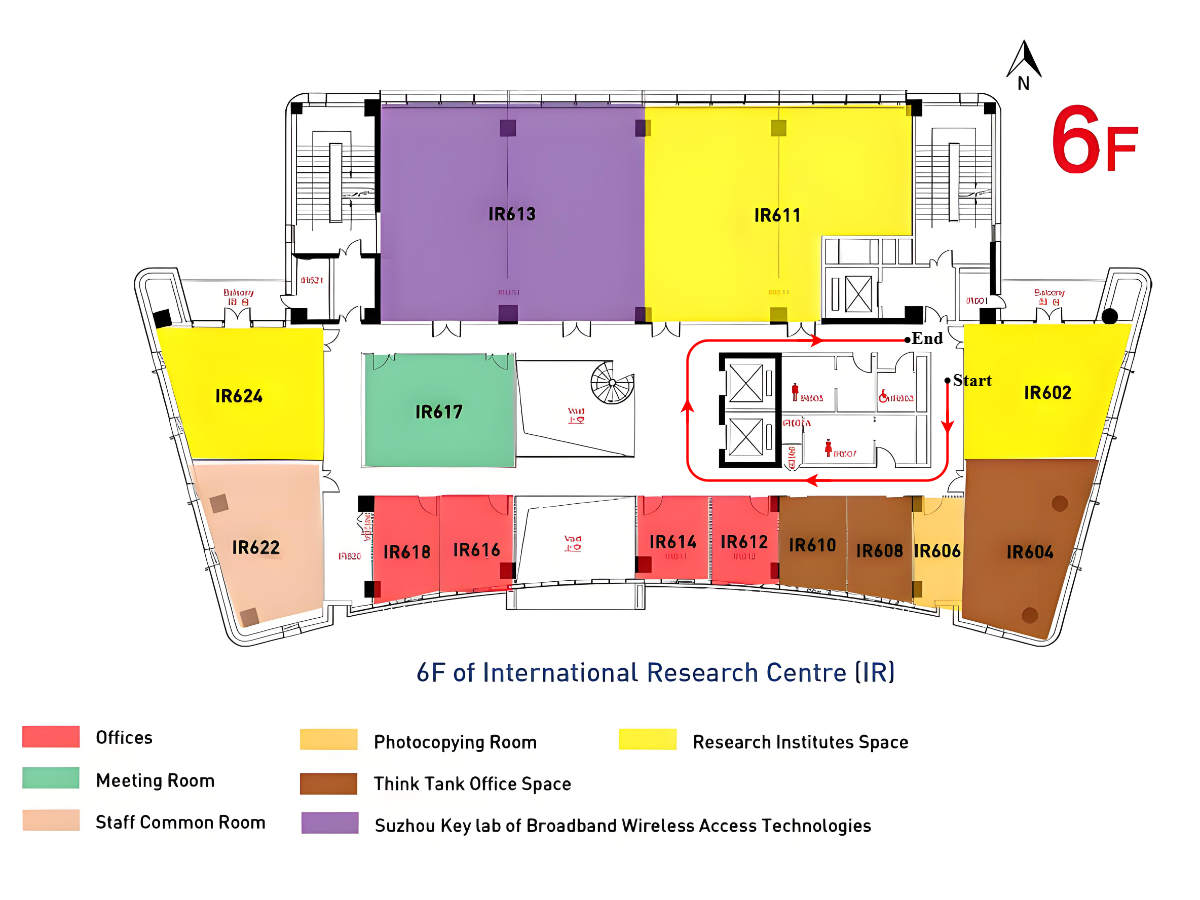
\includegraphics[width=0.8\linewidth]{images/IR_6.drawio (1).png}
  \caption{Localization experiment path on the 6th floor of the IR building.}
  \label{fig:Localization experiment path on the 6th floor of the IR Building}
\end{figure}
\begin{figure}[H]
  \centering
  \includegraphics[width=0.8\linewidth]{images/IR_half_circle.png}
  \caption{Localization experiment path on the 7th floor of the IR building.}
  \label{fig:enter-label}
\end{figure}
\begin{figure}[H]
  \centering
  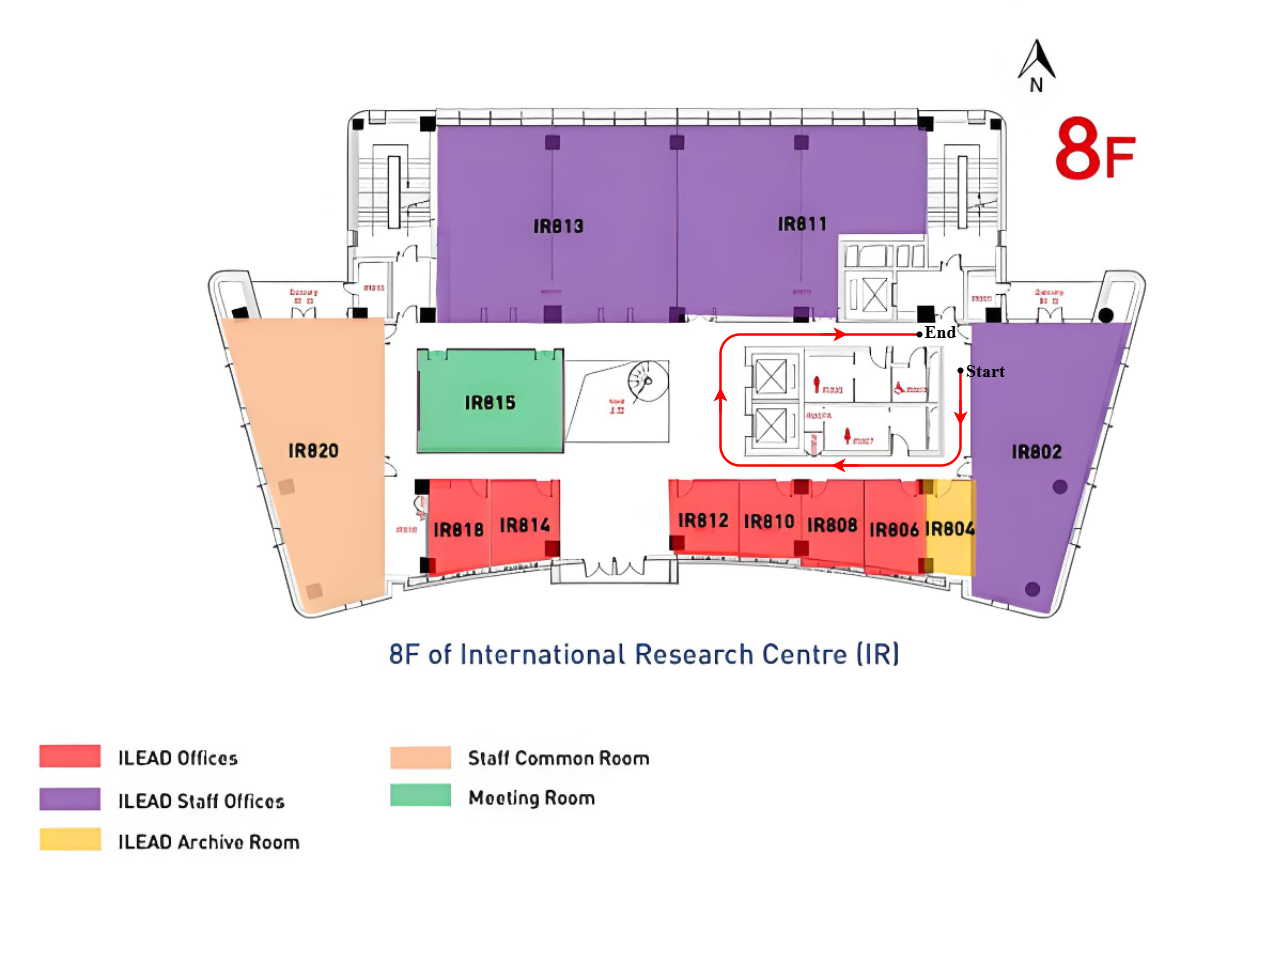
\includegraphics[width=0.9\linewidth]{images/IR_8.drawio (1).png}
  \caption{Localization experiment path on the 8th floor of the IR building.}
  \label{fig:Localization experiment path on the 8th floor of the IR Building}
\end{figure}
  
\section{AGV-Based Data Collection for Sensor Fusion in Indoor Localization}
\begin{figure}[H]
  \centering
  \begin{subfigure}[b]{0.5\textwidth}
    \centering
    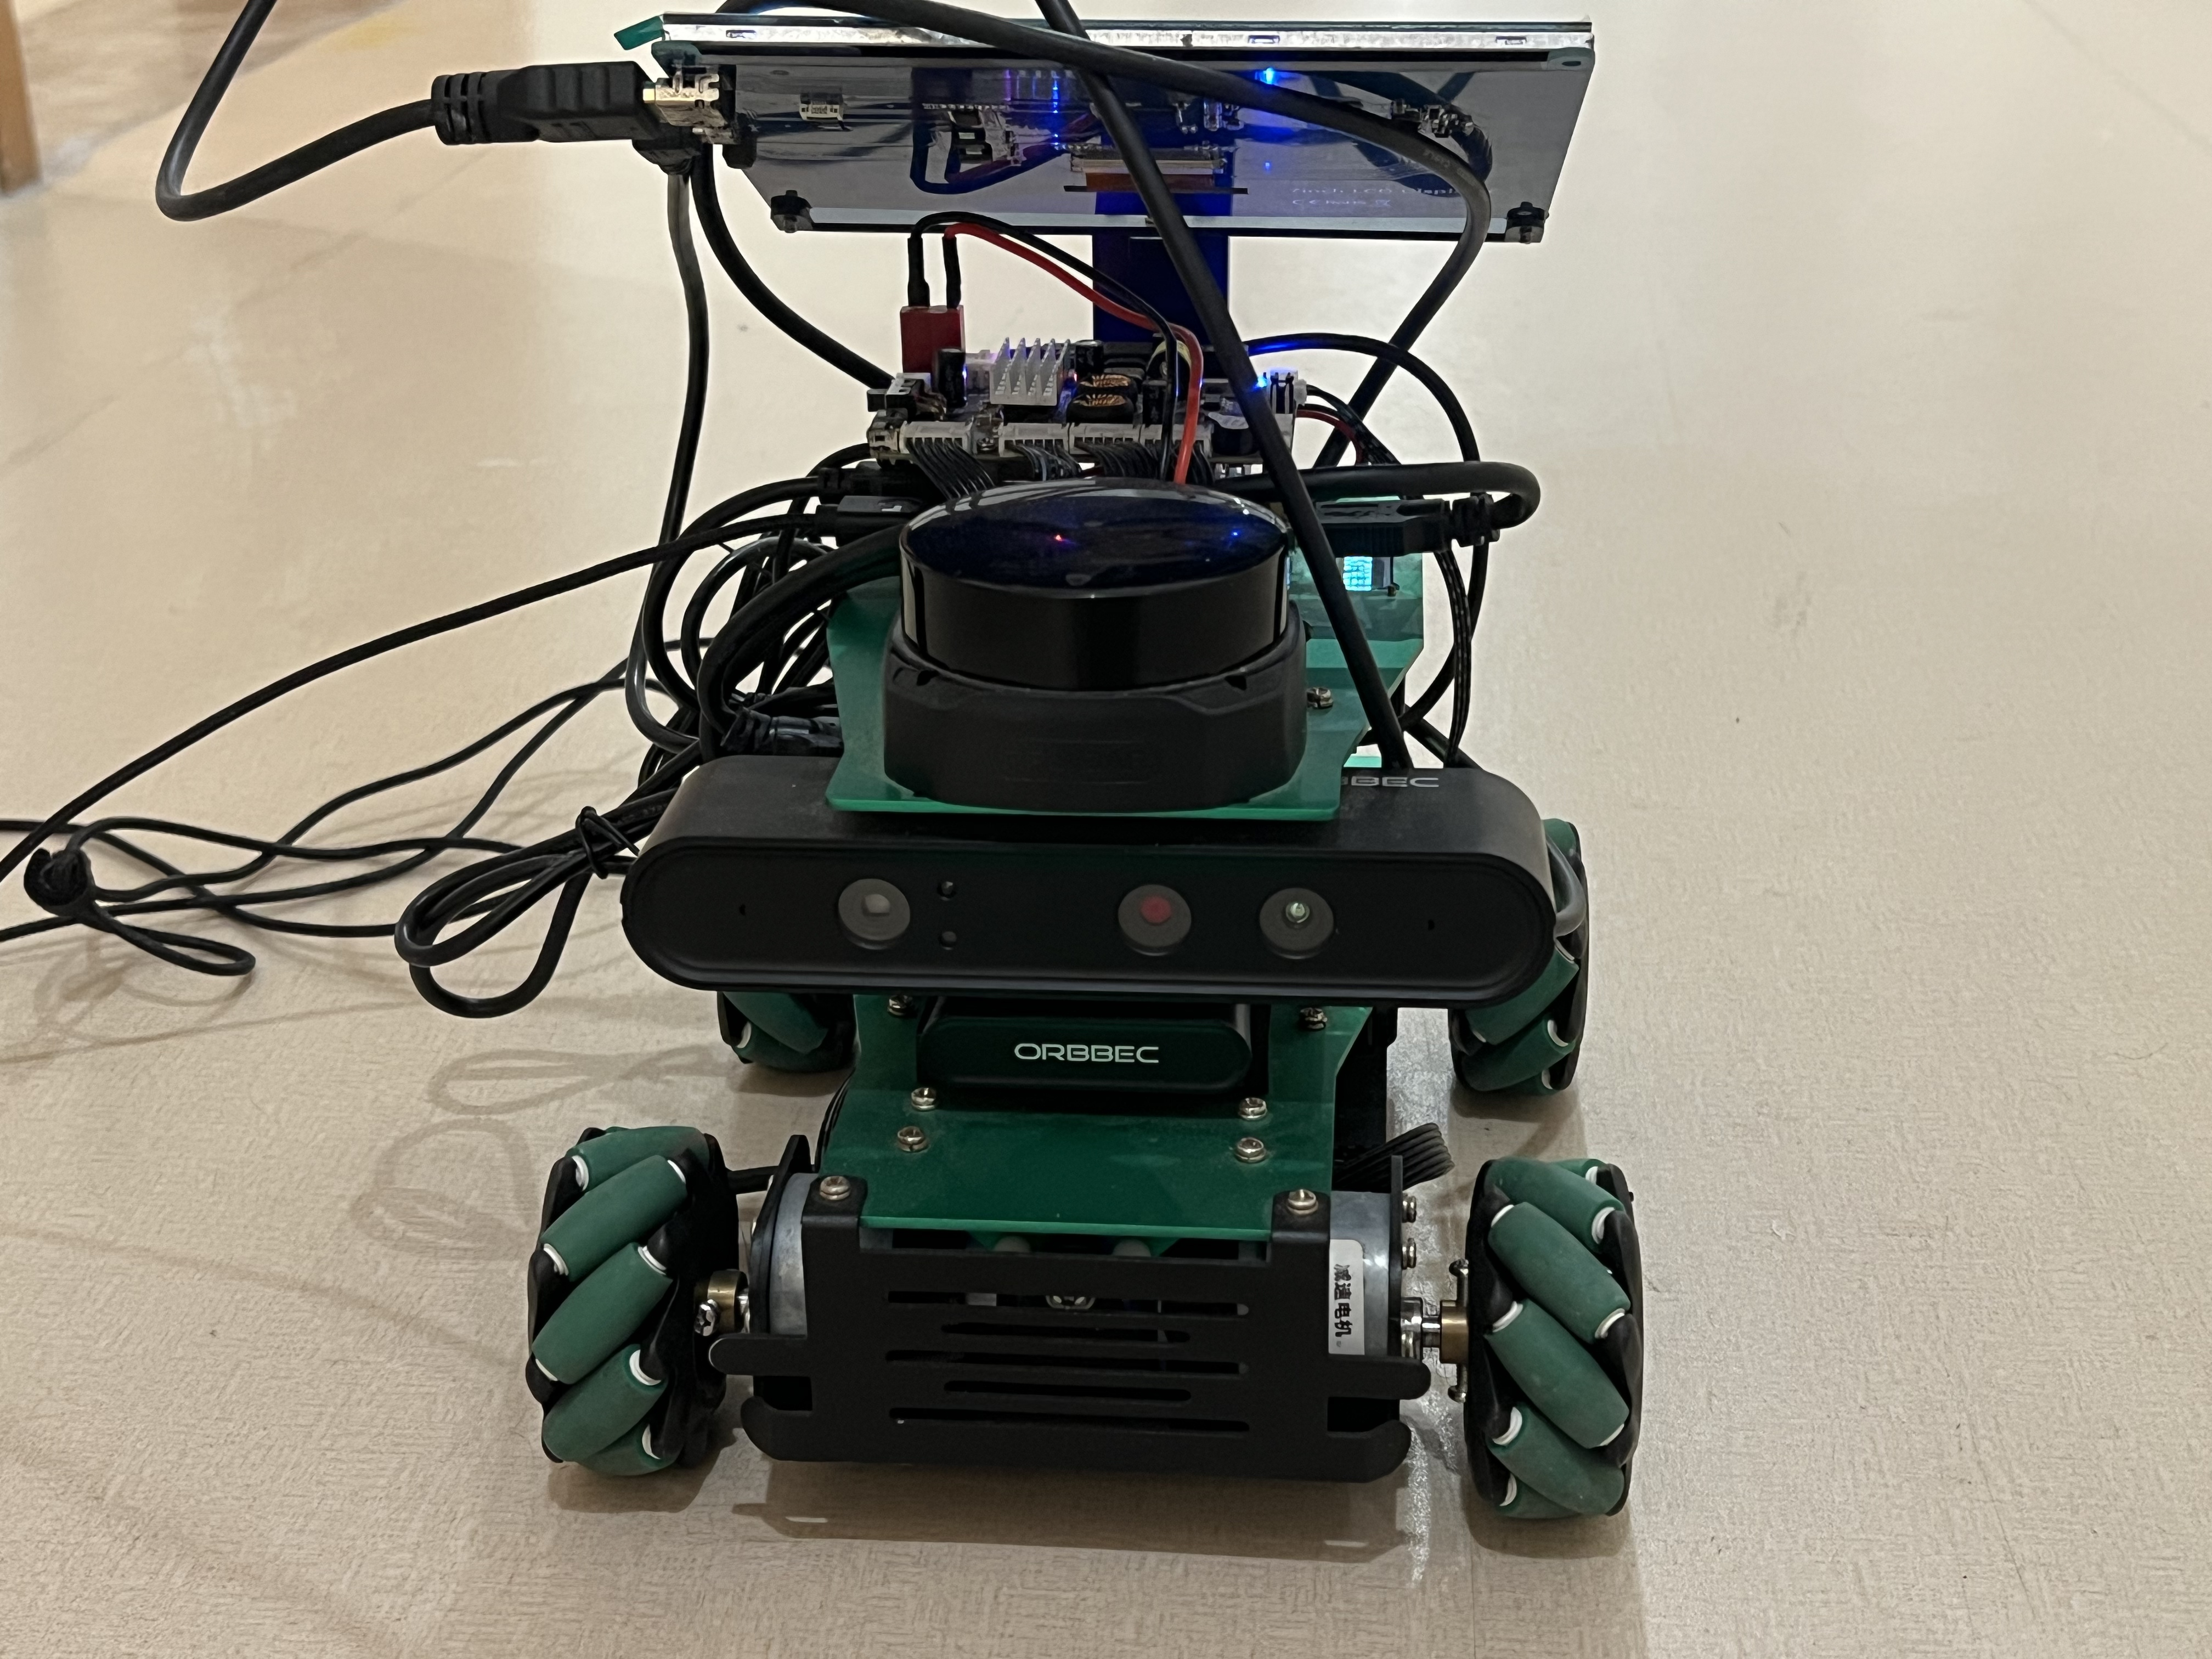
\includegraphics[width=\textwidth]{images/test/1.jpg}
    \caption{}
  \end{subfigure} \hfill
  \begin{subfigure}[b]{0.5\textwidth}
    \centering
    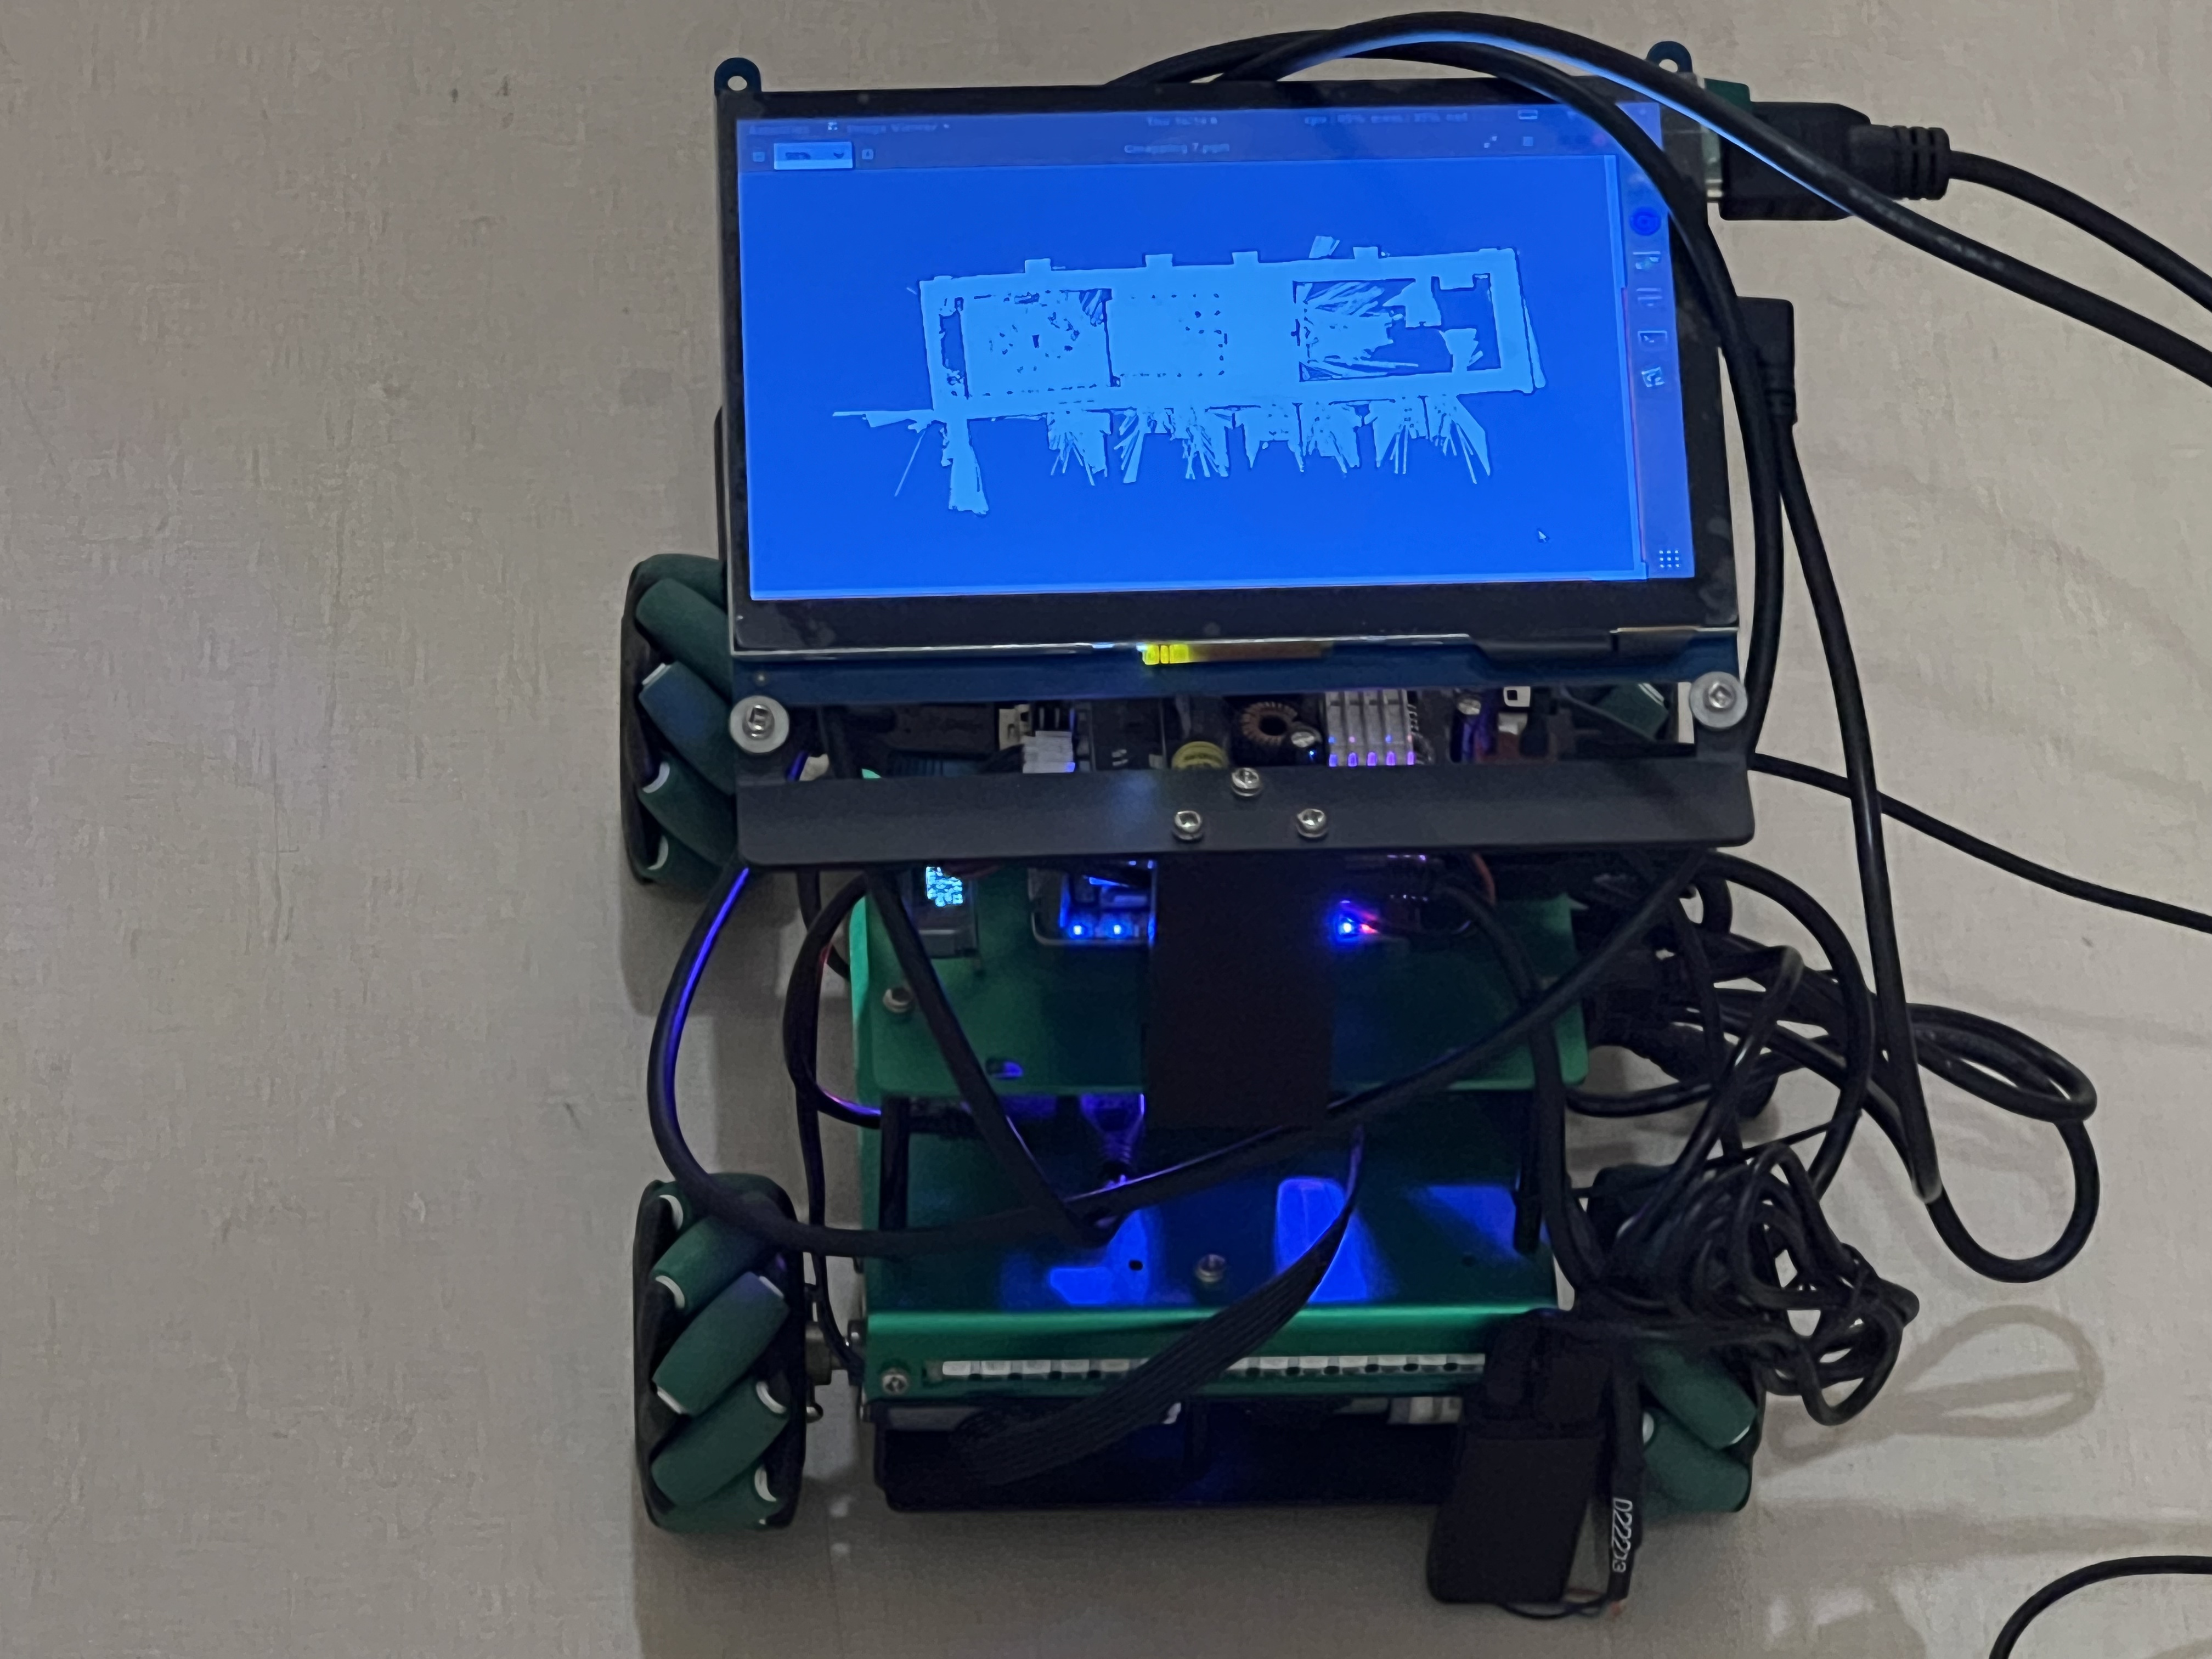
\includegraphics[width=\textwidth]{images/test/2.jpg}
    \caption{}
  \end{subfigure}
  \begin{subfigure}[b]{0.5\textwidth}
    \centering
    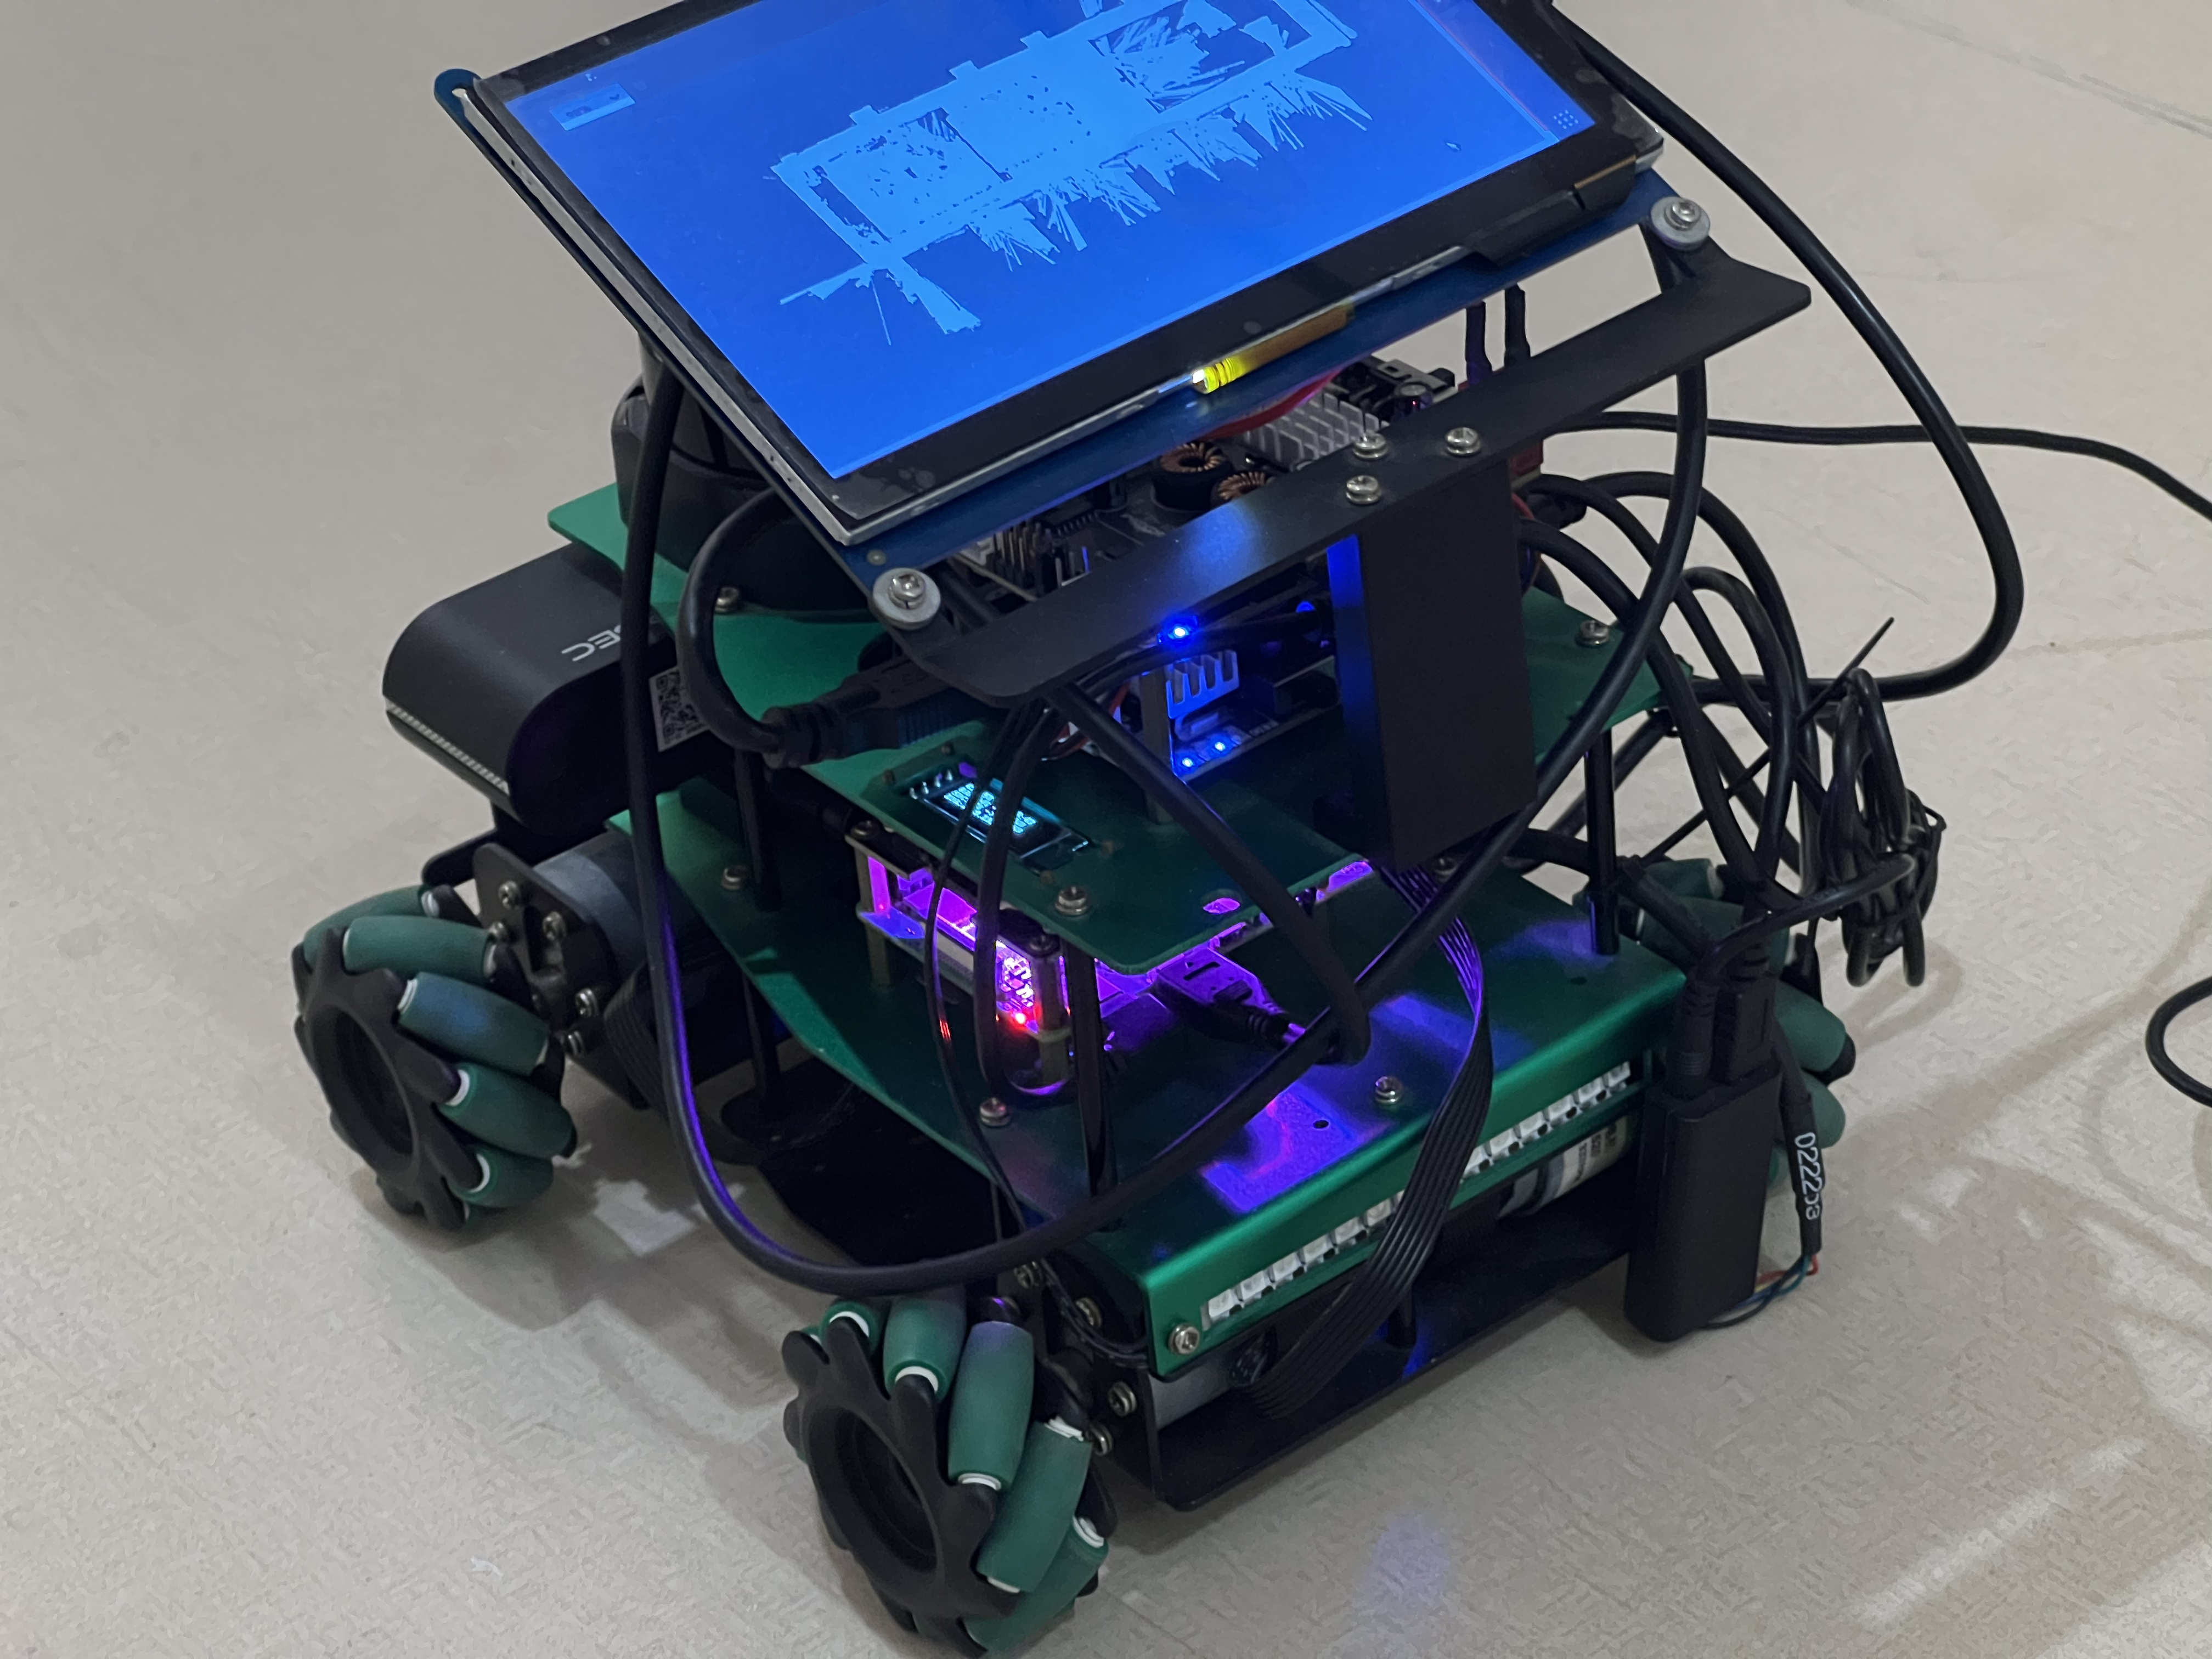
\includegraphics[width=\textwidth]{images/test/3.jpg}
    \caption{}
  \end{subfigure}
  \caption{AGV deployment for indoor localization using Wi-Fi and LiDAR fusion:
    (a) \textcolor{red}{add description}, (b) \textcolor{red}{add description},
    and (c) \textcolor{red}{add description}.}
  %%% 
  \comment{Joseph}{Provide descriptions for (a), (b), and (c).}%
  %%% 
\end{figure}


\end{document}
